
\section{Benchmark CG}
\subsection{Wyniki benchmarków - platforma ARM64}

\begin{figure}[H]
    \centering
    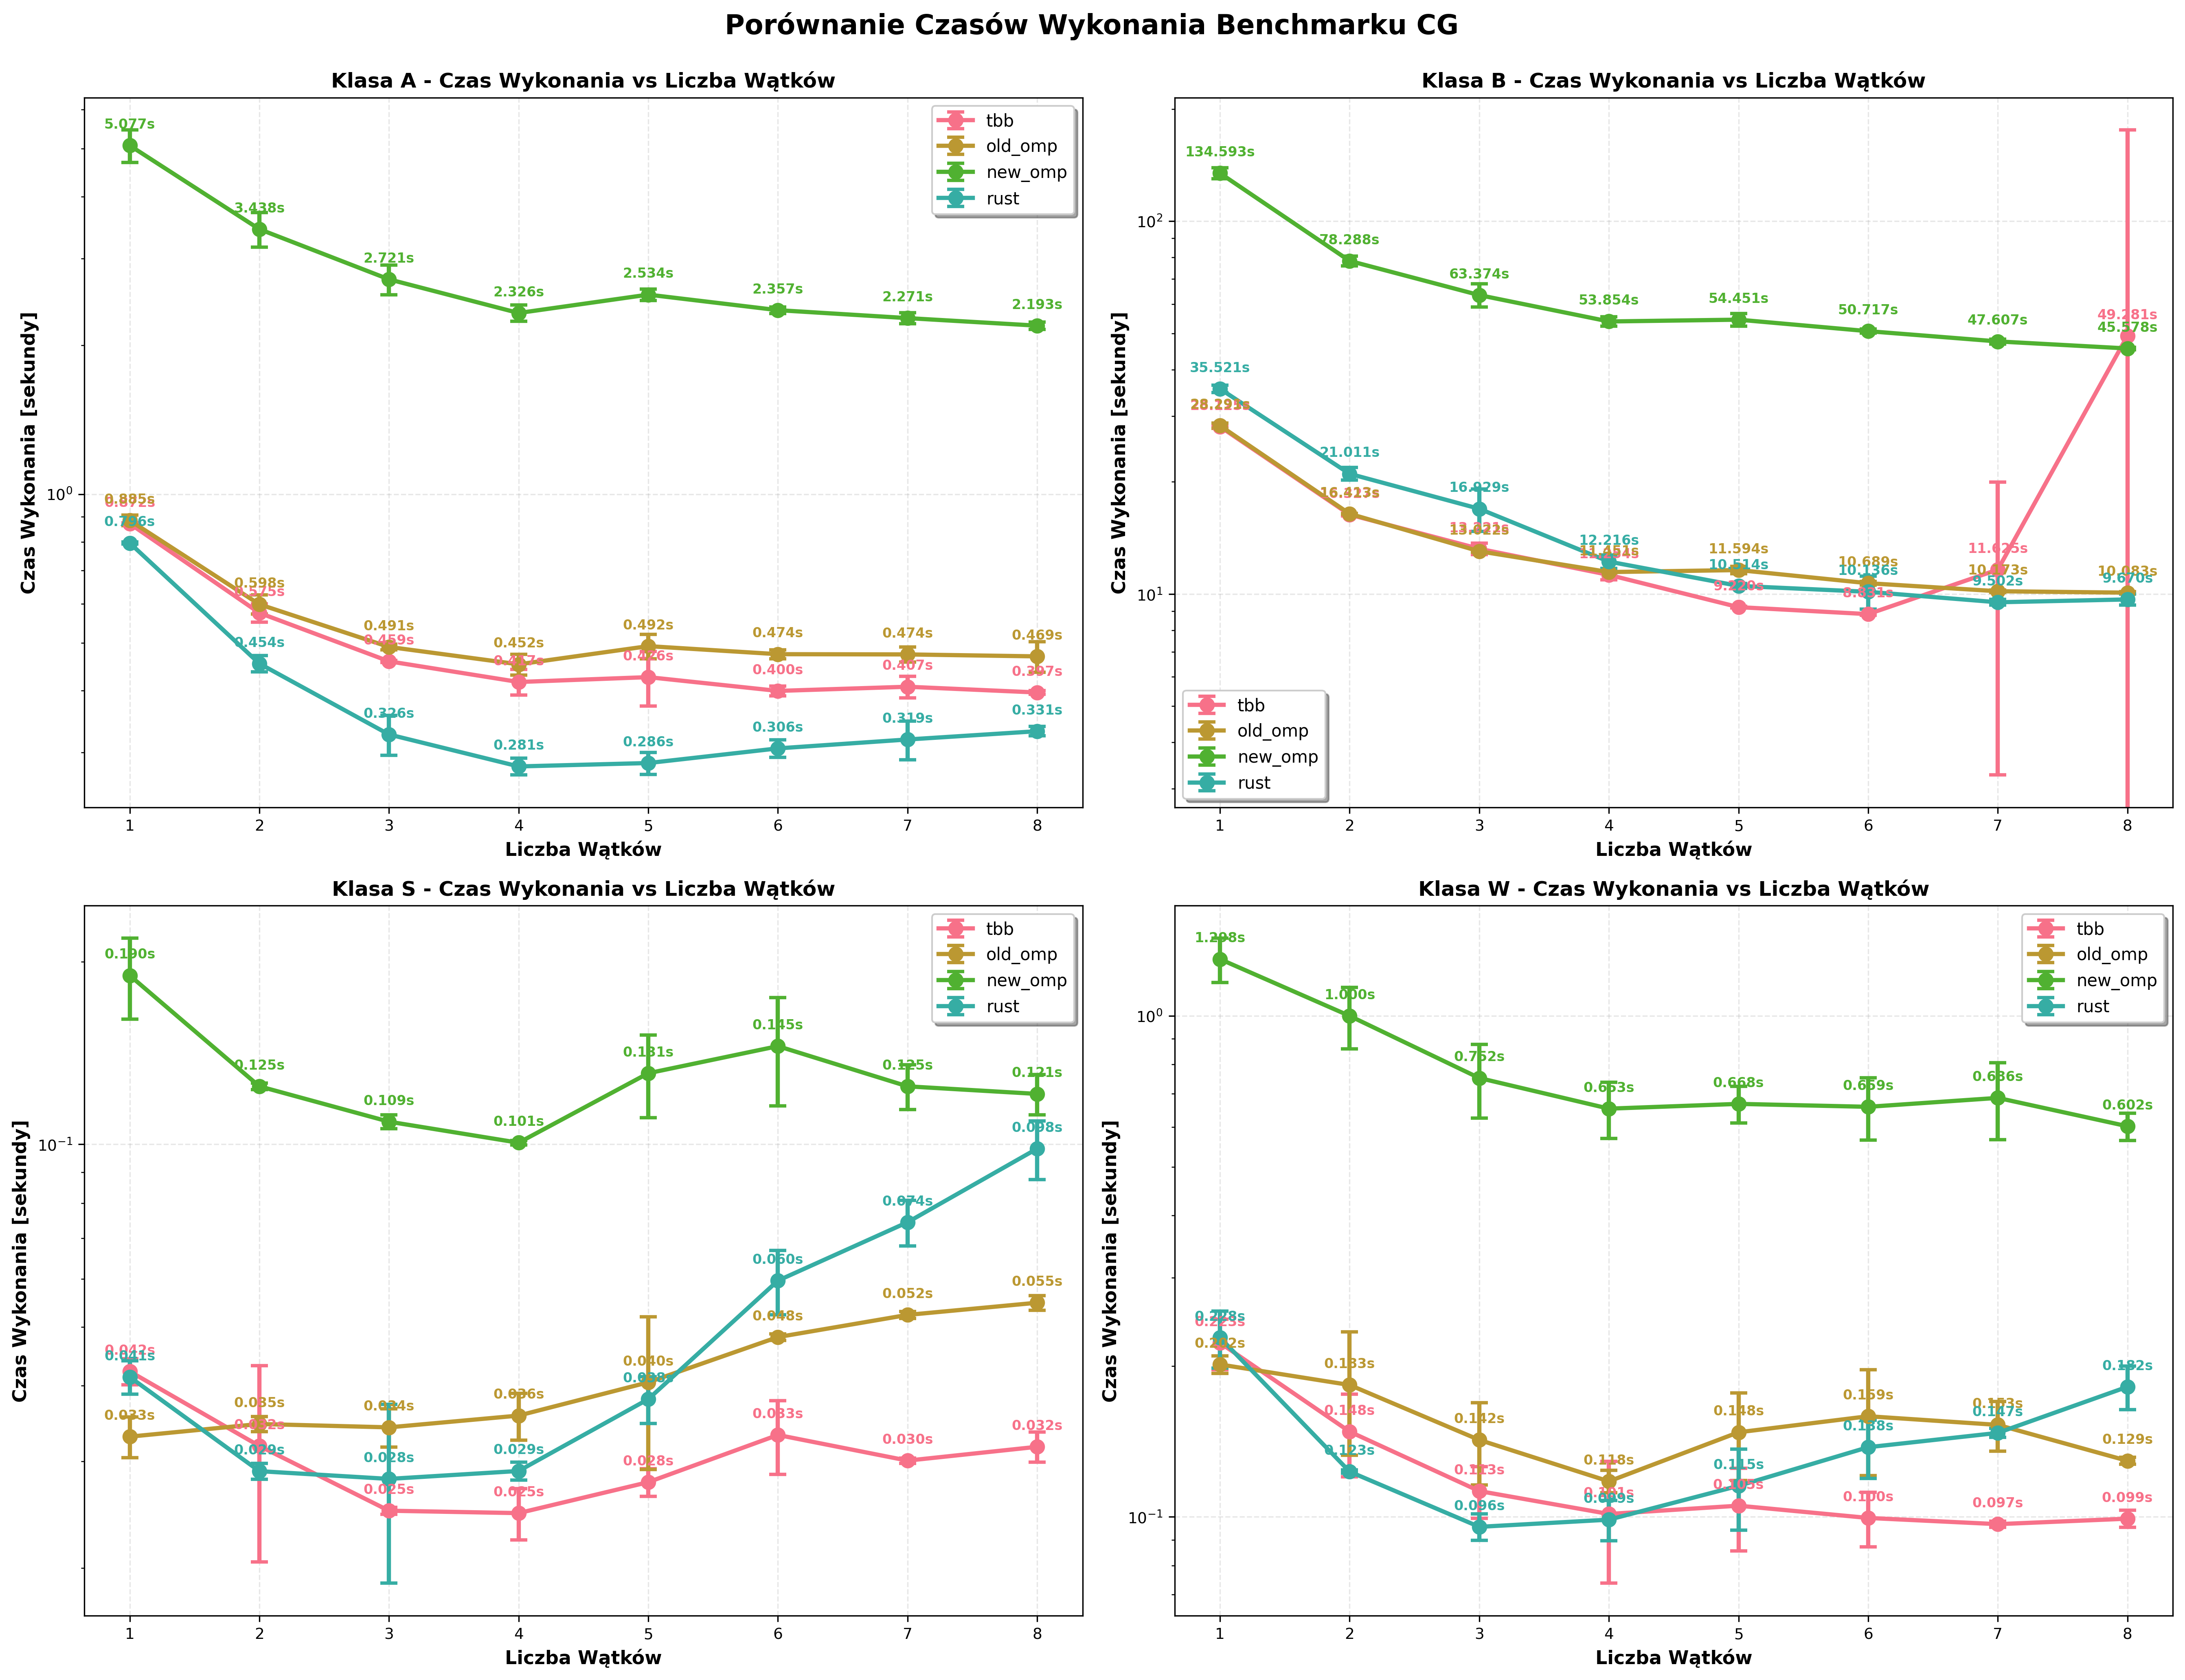
\includegraphics[width=\textwidth]{analiza/images/parallel/cg/arm/cg_porownanie_czasow_wykonania.png}
    \caption{Porównanie czasów wykonania benchmarku CG dla klas S, W, A, B względem liczby użytych wątków na platformie ARM64}
    \label{cg_porownanie_czasow_wykonania}
\end{figure}

Na rysunku \ref{cg_porownanie_czasow_wykonania} zaprezentowano zestawienie czasów wykonania benchmarku CG dla czterech klas problemu: S, W, A oraz B, przy użyciu czterech różnych implementacji równoległości: TBB, OpenMP w wersji oryginalnej w stylu języka Fortran (old\_omp), OpenMP w wersji nowszej (new\_omp) oraz implementacji w języku Rust. Dla każdej z klas przedstawiono zależność czasu wykonania od liczby wątków (od 1 do 8). Wartości zostały zaprezentowane w skali logarytmicznej.

\begin{figure}[H]
    \centering
    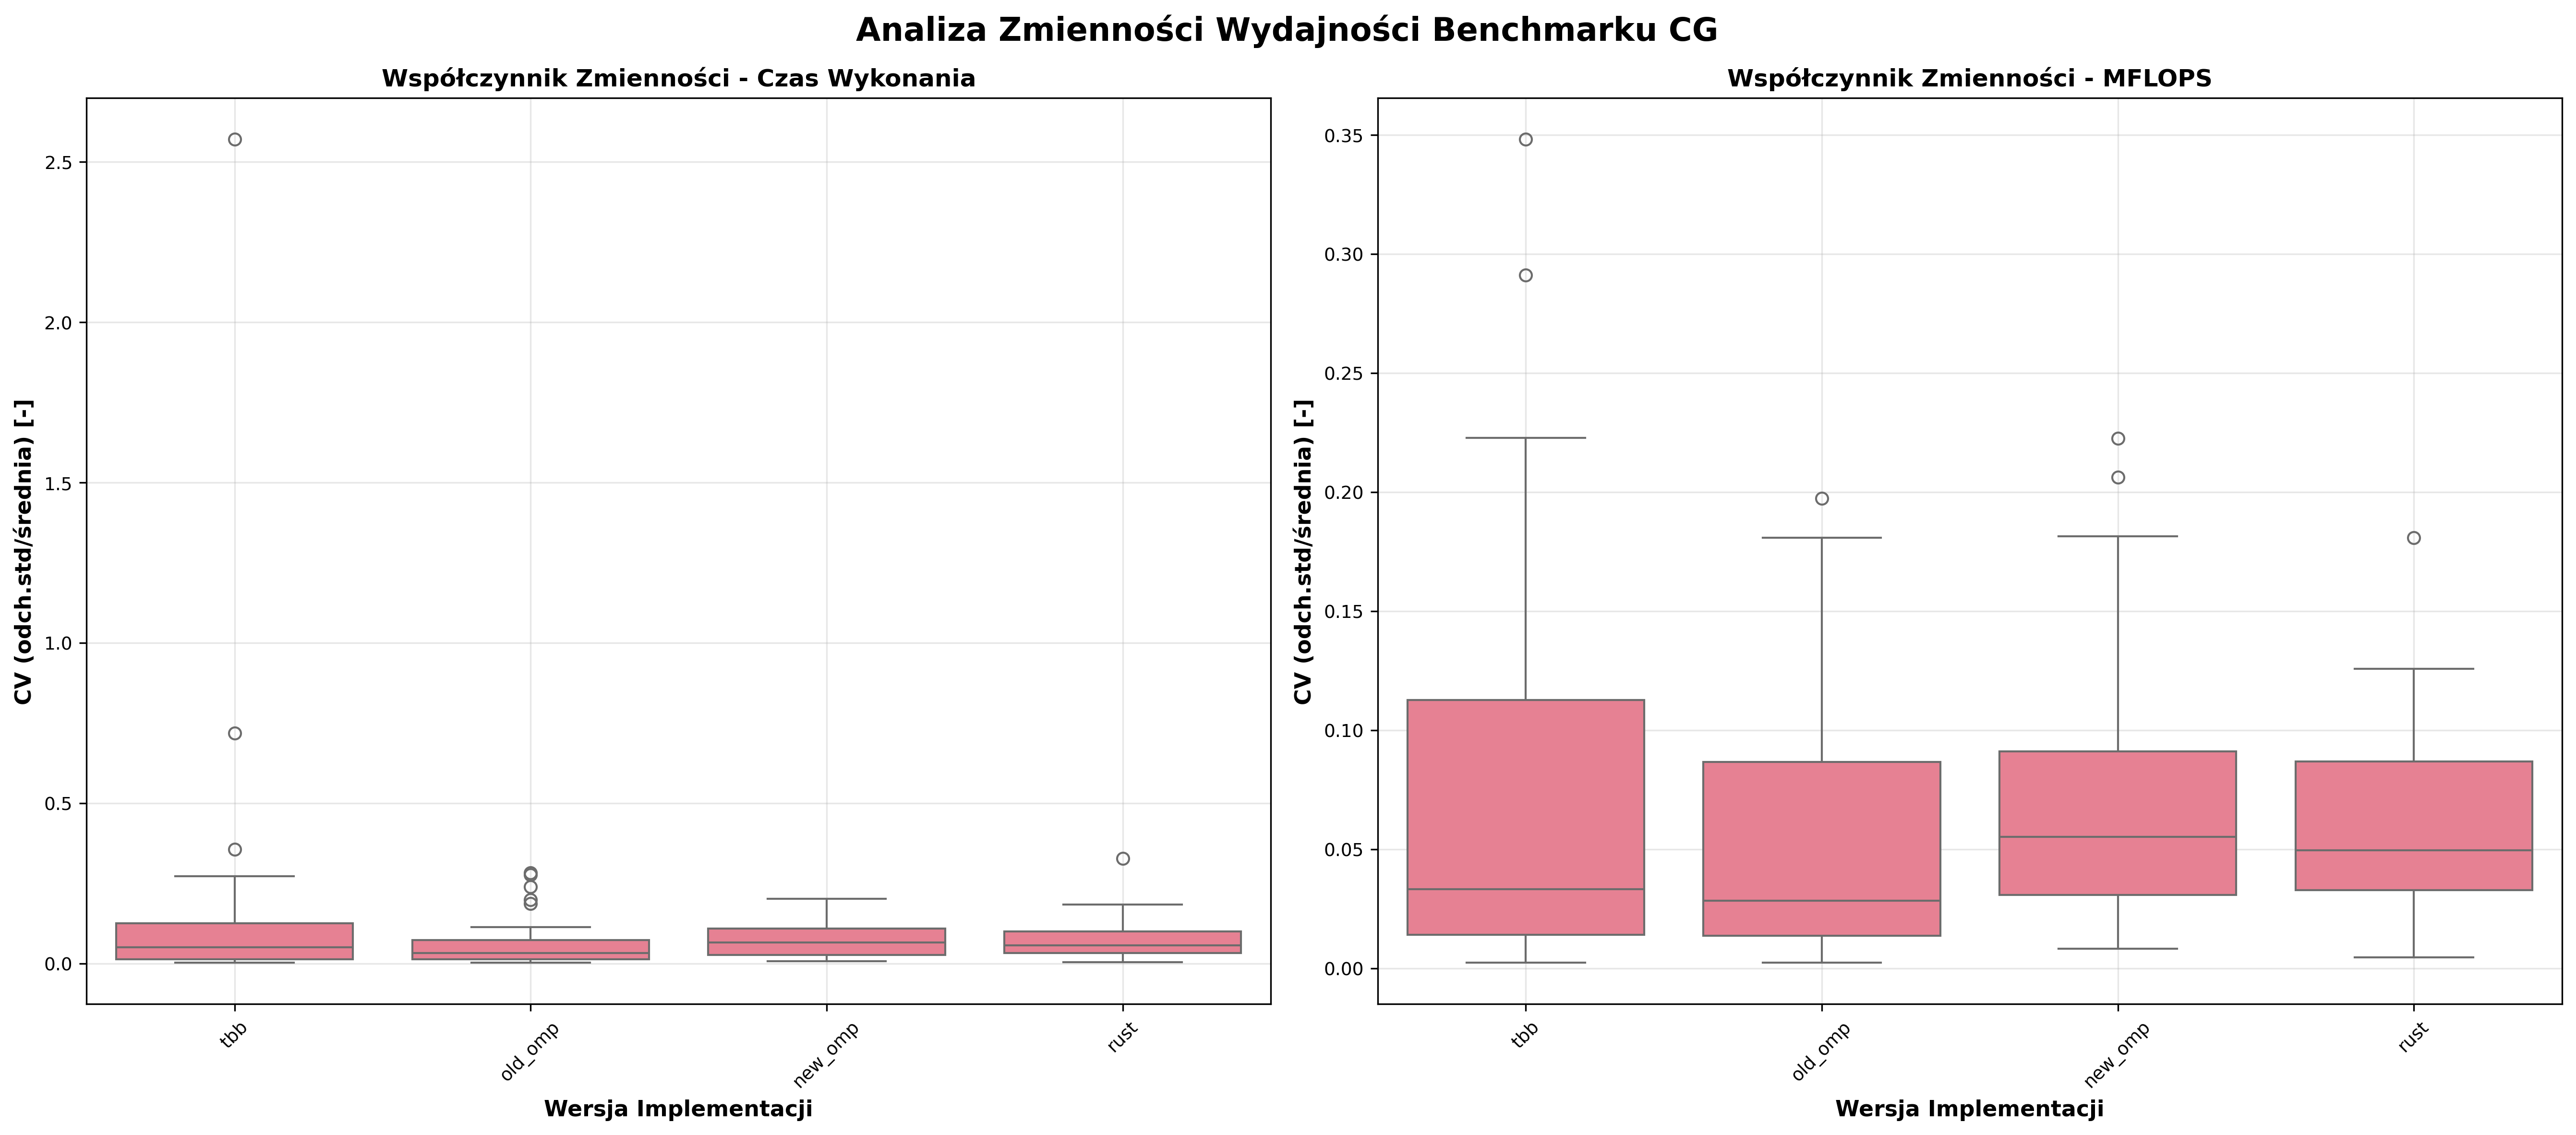
\includegraphics[width=\textwidth]{analiza/images/parallel/cg/arm/cg_analiza_zmiennosci.png}
    \caption{Analiza zmienności czasów wykonania benchmarku CG dla klas S, W, A, B względem liczby użytych wątków na platformie ARM64}
    \label{cg_analiza_zmiennosci}
\end{figure}
Powyższy wykres - rysunek \ref{cg_analiza_zmiennosci} pudełkowy prezentuje współczynnik zmienności \eng{CV - coefficient of variation}, obliczony jako stosunek odchylenia standardowego do wartości średniej, w odniesieniu do czasu wykonania (lewy wykres) oraz uzyskiwanej wydajności (prawy wykres) dla różnych wersji implementacji benchmarku.

\subsubsection{Klasa A}
Dla klasy A obserwuje się istotne skrócenie czasu wykonania w miarę zwiększania liczby wątków we wszystkich implementacjach. Najlepsze wyniki osiąga implementacja w języku Rust, która przy dwóch wątkach wykazuje już znaczną poprawę, a dalsze zwiększanie liczby wątków prowadzi do stopniowego, choć już mniej dynamicznego, spadku czasu wykonania. Implementacje oparte na TBB oraz new\_omp osiągają porównywalne wyniki, przy czym TBB zyskuje przewagę przy większej liczbie wątków. old\_omp charakteryzuje się najmniejszą efektywnością spośród rozważanych technologii

\subsubsection{Klasa B}
W przypadku klasy B, reprezentującej znacznie większy problem obliczeniowy, wszystkie implementacje wykazują duże korzyści z równoległości do około 4-5 wątków. Najlepsze rezultaty osiąga new\_omp oraz Rust, które utrzymują stabilny i niski czas wykonania dla większej liczby wątków. Implementacja TBB wykazuje niejednorodne zachowanie, a przy 8 wątkach dochodzi do gwałtownego wzrostu czasu wykonania i odchylenia standardowego, co może świadczyć o problemach z równoważeniem obciążenia \eng{load balancing}. old\_omp stabilizuje się przy wyższym poziomie czasów wykonania, ale nie wykazuje znaczącej degradacji.

\subsubsection{Klasa S}
Dla klasy S, reprezentującej mały problem obliczeniowy, dominująca jest implementacja w języku Rust, osiągająca najniższe czasy wykonania dla niemal wszystkich liczby wątków. Warto zauważyć, że dla tej klasy problemu korzyści ze zwiększania liczby wątków są ograniczone, a różnice pomiędzy implementacjami są bardziej subtelne. TBB oraz new\_omp oferują porównywalne wyniki, podczas gdy old\_omp utrzymuje wyższe wartości czasów, co sugeruje niższą efektywność dla małych problemów.

\subsubsection{Klasa W}
Dla klasy W obserwuje się podobny trend jak w klasie S, lecz z bardziej widoczną poprawą wydajności przy zwiększaniu liczby wątków. Rust oraz TBB osiągają najniższe czasy wykonania, z przewagą Rusta przy mniejszej liczbie wątków oraz TBB dla konfiguracji 6-8 wątków. old\_omp po raz kolejny okazuje się najmniej wydajnym rozwiązaniem. new\_omp wykazuje stabilne, ale umiarkowane czasy wykonania.

\subsubsection{Współczynnik zmienności - czas wykonania}
Na lewym wykresie - rysunek \ref{cg_analiza_zmiennosci} zaobserwować można, że implementacja tbb cechuje się najwyższą zmiennością czasu wykonania. Występują dla niej wartości odstające dochodzące nawet do CV > 2.5, co może wskazywać na niestabilność działania w wybranych konfiguracjach (np. liczba wątków lub klasa problemu). Mediana wartości CV dla tbb pozostaje jednak niska, co oznacza, że większość przypadków wykazuje umiarkowaną stabilność.

Pozostałe implementacje (old\_omp, new\_omp, rust) charakteryzują się wyraźnie niższą zmiennością czasu wykonania. Dla old\_omp widocznych jest kilka wartości odstających, ale ogólny rozkład jest bardziej zwarty. new\_omp i rust prezentują podobny poziom zmienności, z medianami bliskimi zera i niewielką rozpiętością wartości, co potwierdza ich stabilność obliczeniową.

\subsubsection{Współczynnik zmienności - MFLOPS}
Na prawym wykresie - rysunek \ref{cg_analiza_zmiennosci} porównano zmienność względną wydajności mierzonej w MFLOPS. Również tutaj tbb wykazuje najwyższy rozrzut wyników, z wieloma obserwacjami odstającymi, choć mediana nadal pozostaje niska (około 0.03). Może to oznaczać, że w specyficznych warunkach (np. przy większym obciążeniu systemu) tbb jest podatne na spadki wydajności.

W przypadku old\_omp, new\_omp i rust rozkłady CV są bardziej zwarte. rust oraz new\_omp mają bardzo zbliżone mediany (~0.03-0.04) i umiarkowaną zmienność, co wskazuje na przewidywalność osiąganej wydajności. old\_omp, mimo że często charakteryzował się niższą bezwzględną wydajnością (jak pokazano w poprzednich analizach), okazuje się względnie stabilny w kontekście MFLOPS.
%------------------------------

\begin{figure}[H]
    \centering
    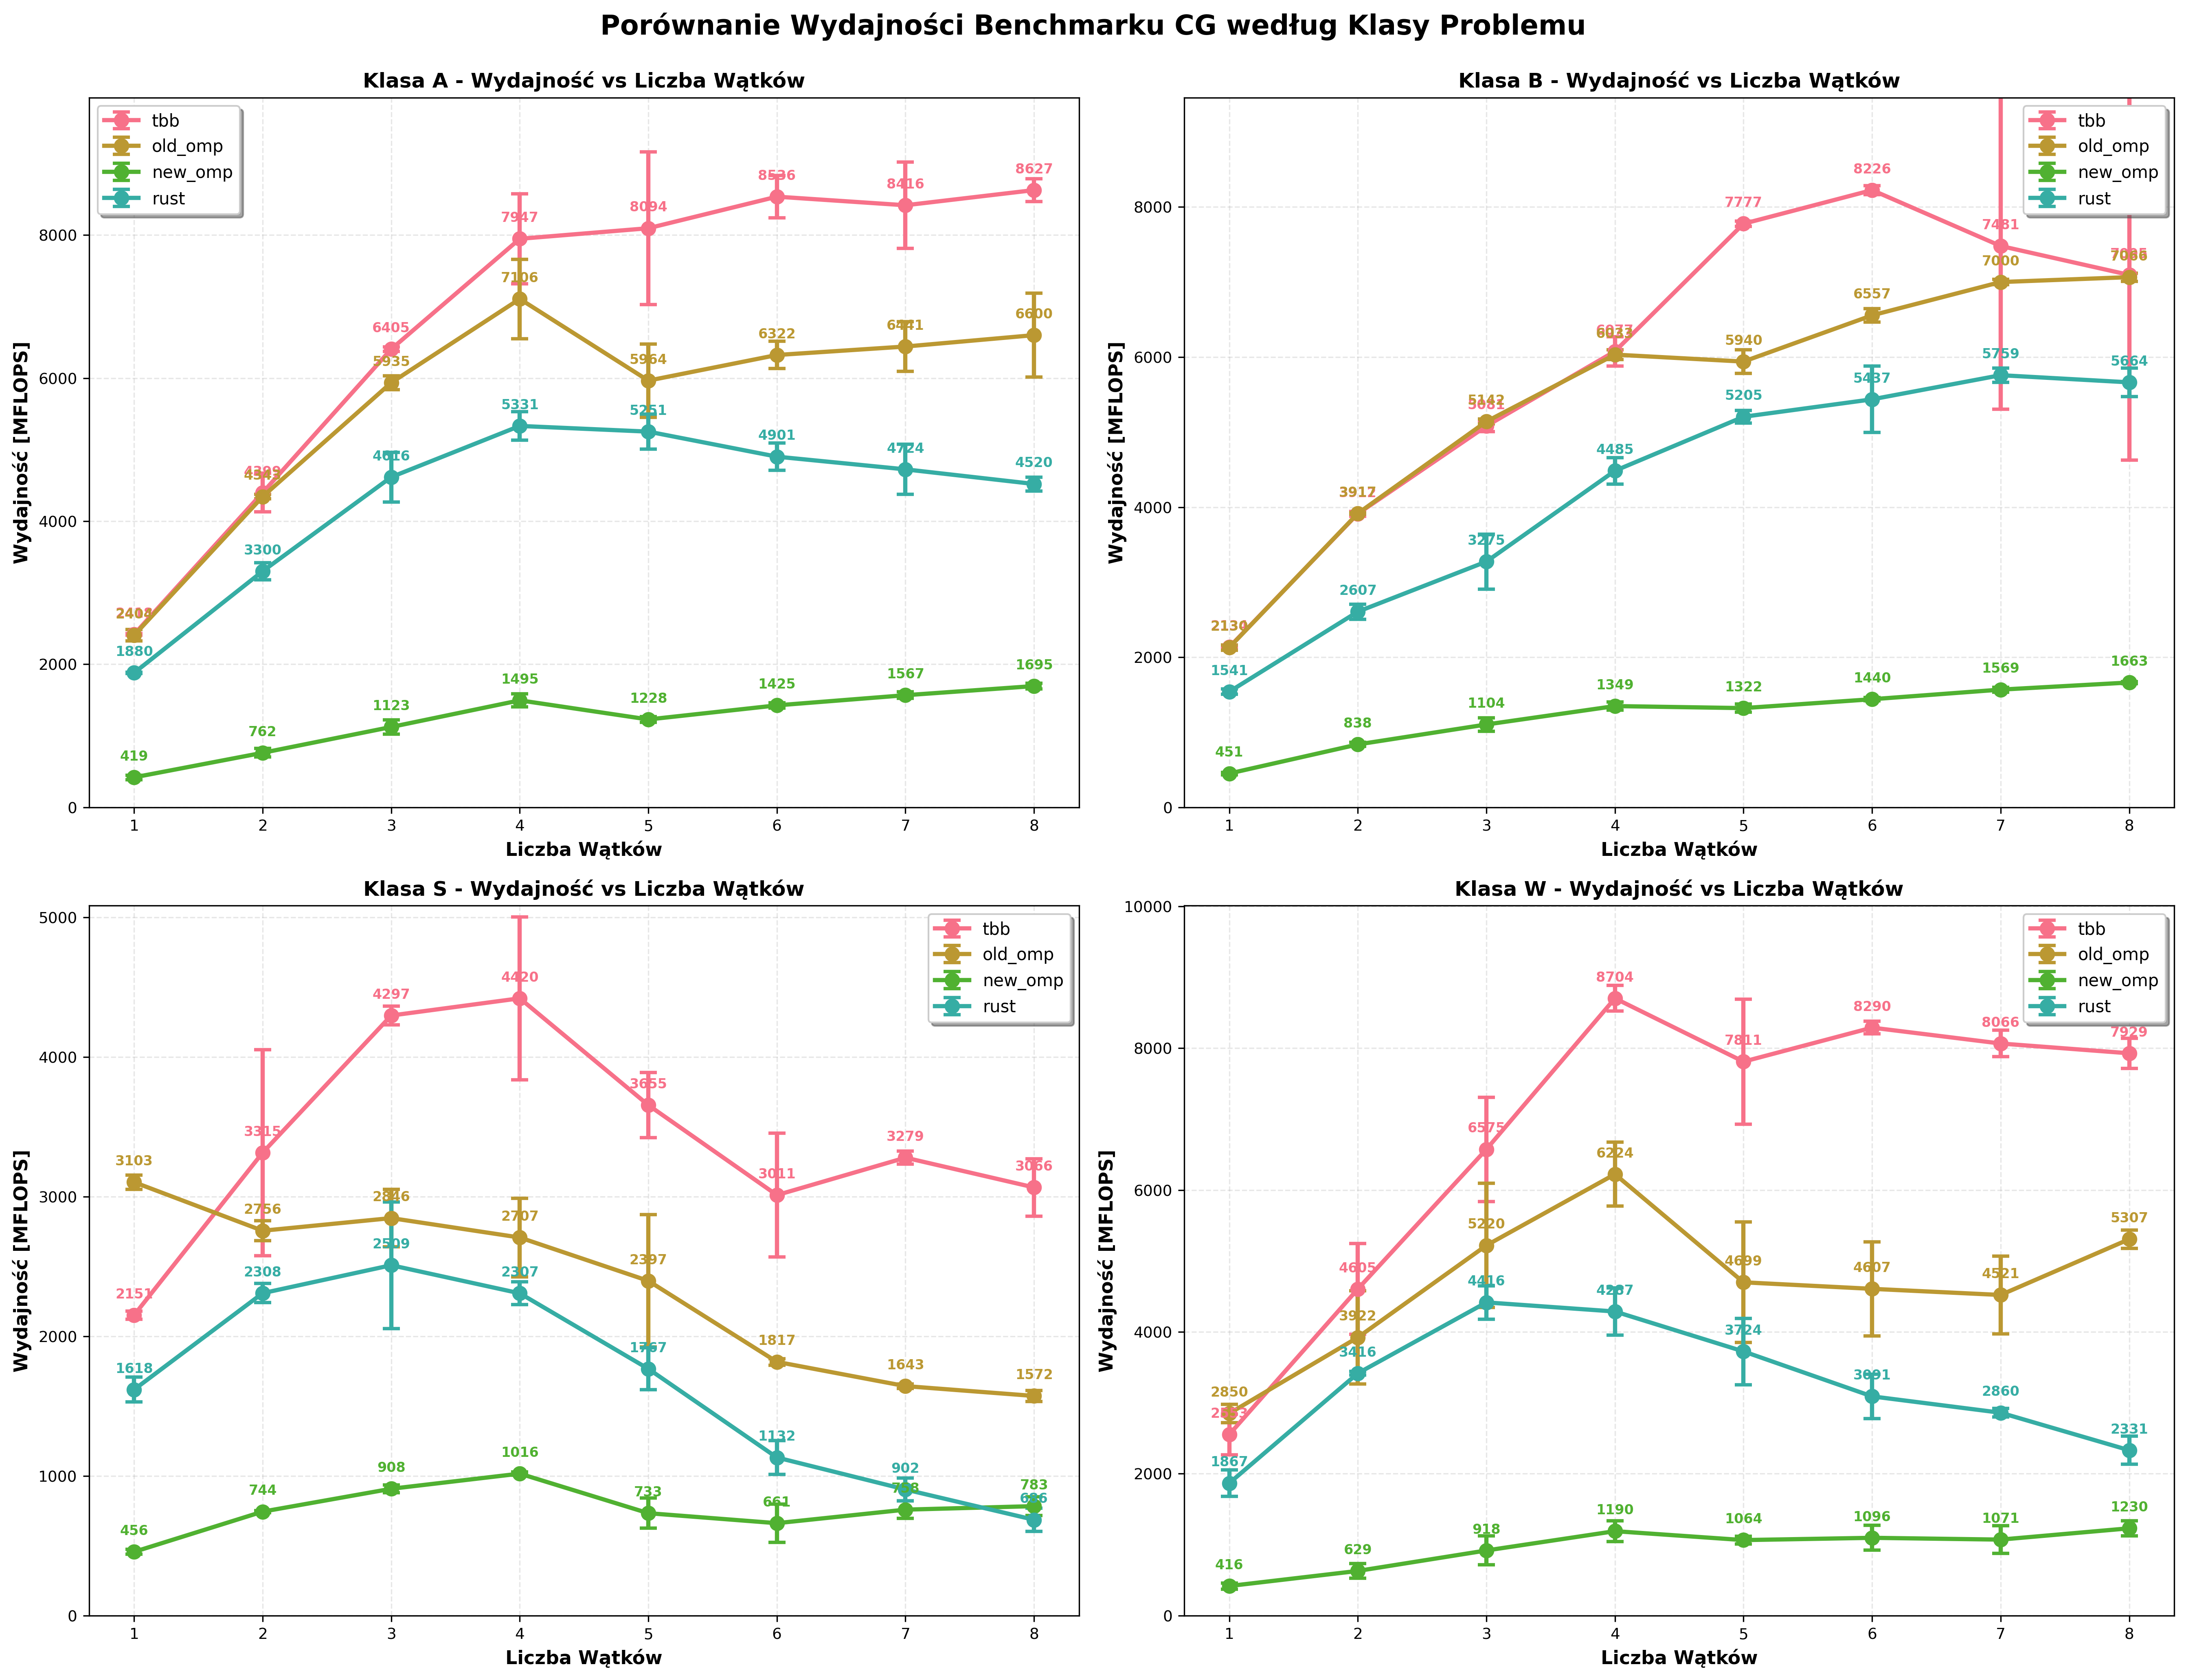
\includegraphics[width=\textwidth]{analiza/images/parallel/cg/arm/cg_porownanie_wydajnosci.png}
    \caption{Porównanie wydajności benchmarku CG dla klas S, W, A, B względem liczby użytych wątków na platformie ARM64}
    \label{cg_porownanie_wydajnosci}
\end{figure}
Na wykresach na rysunku \ref{cg_porownanie_wydajnosci} zaprezentowano porównanie wydajności benchmarku CG mierzonej w MFLOPS (milionach operacji zmiennoprzecinkowych na sekundę). Wydajność została przedstawiona jako funkcja liczby wątków (1-8) dla czterech implementacji równoległych.

\begin{figure}[H]
    \centering
    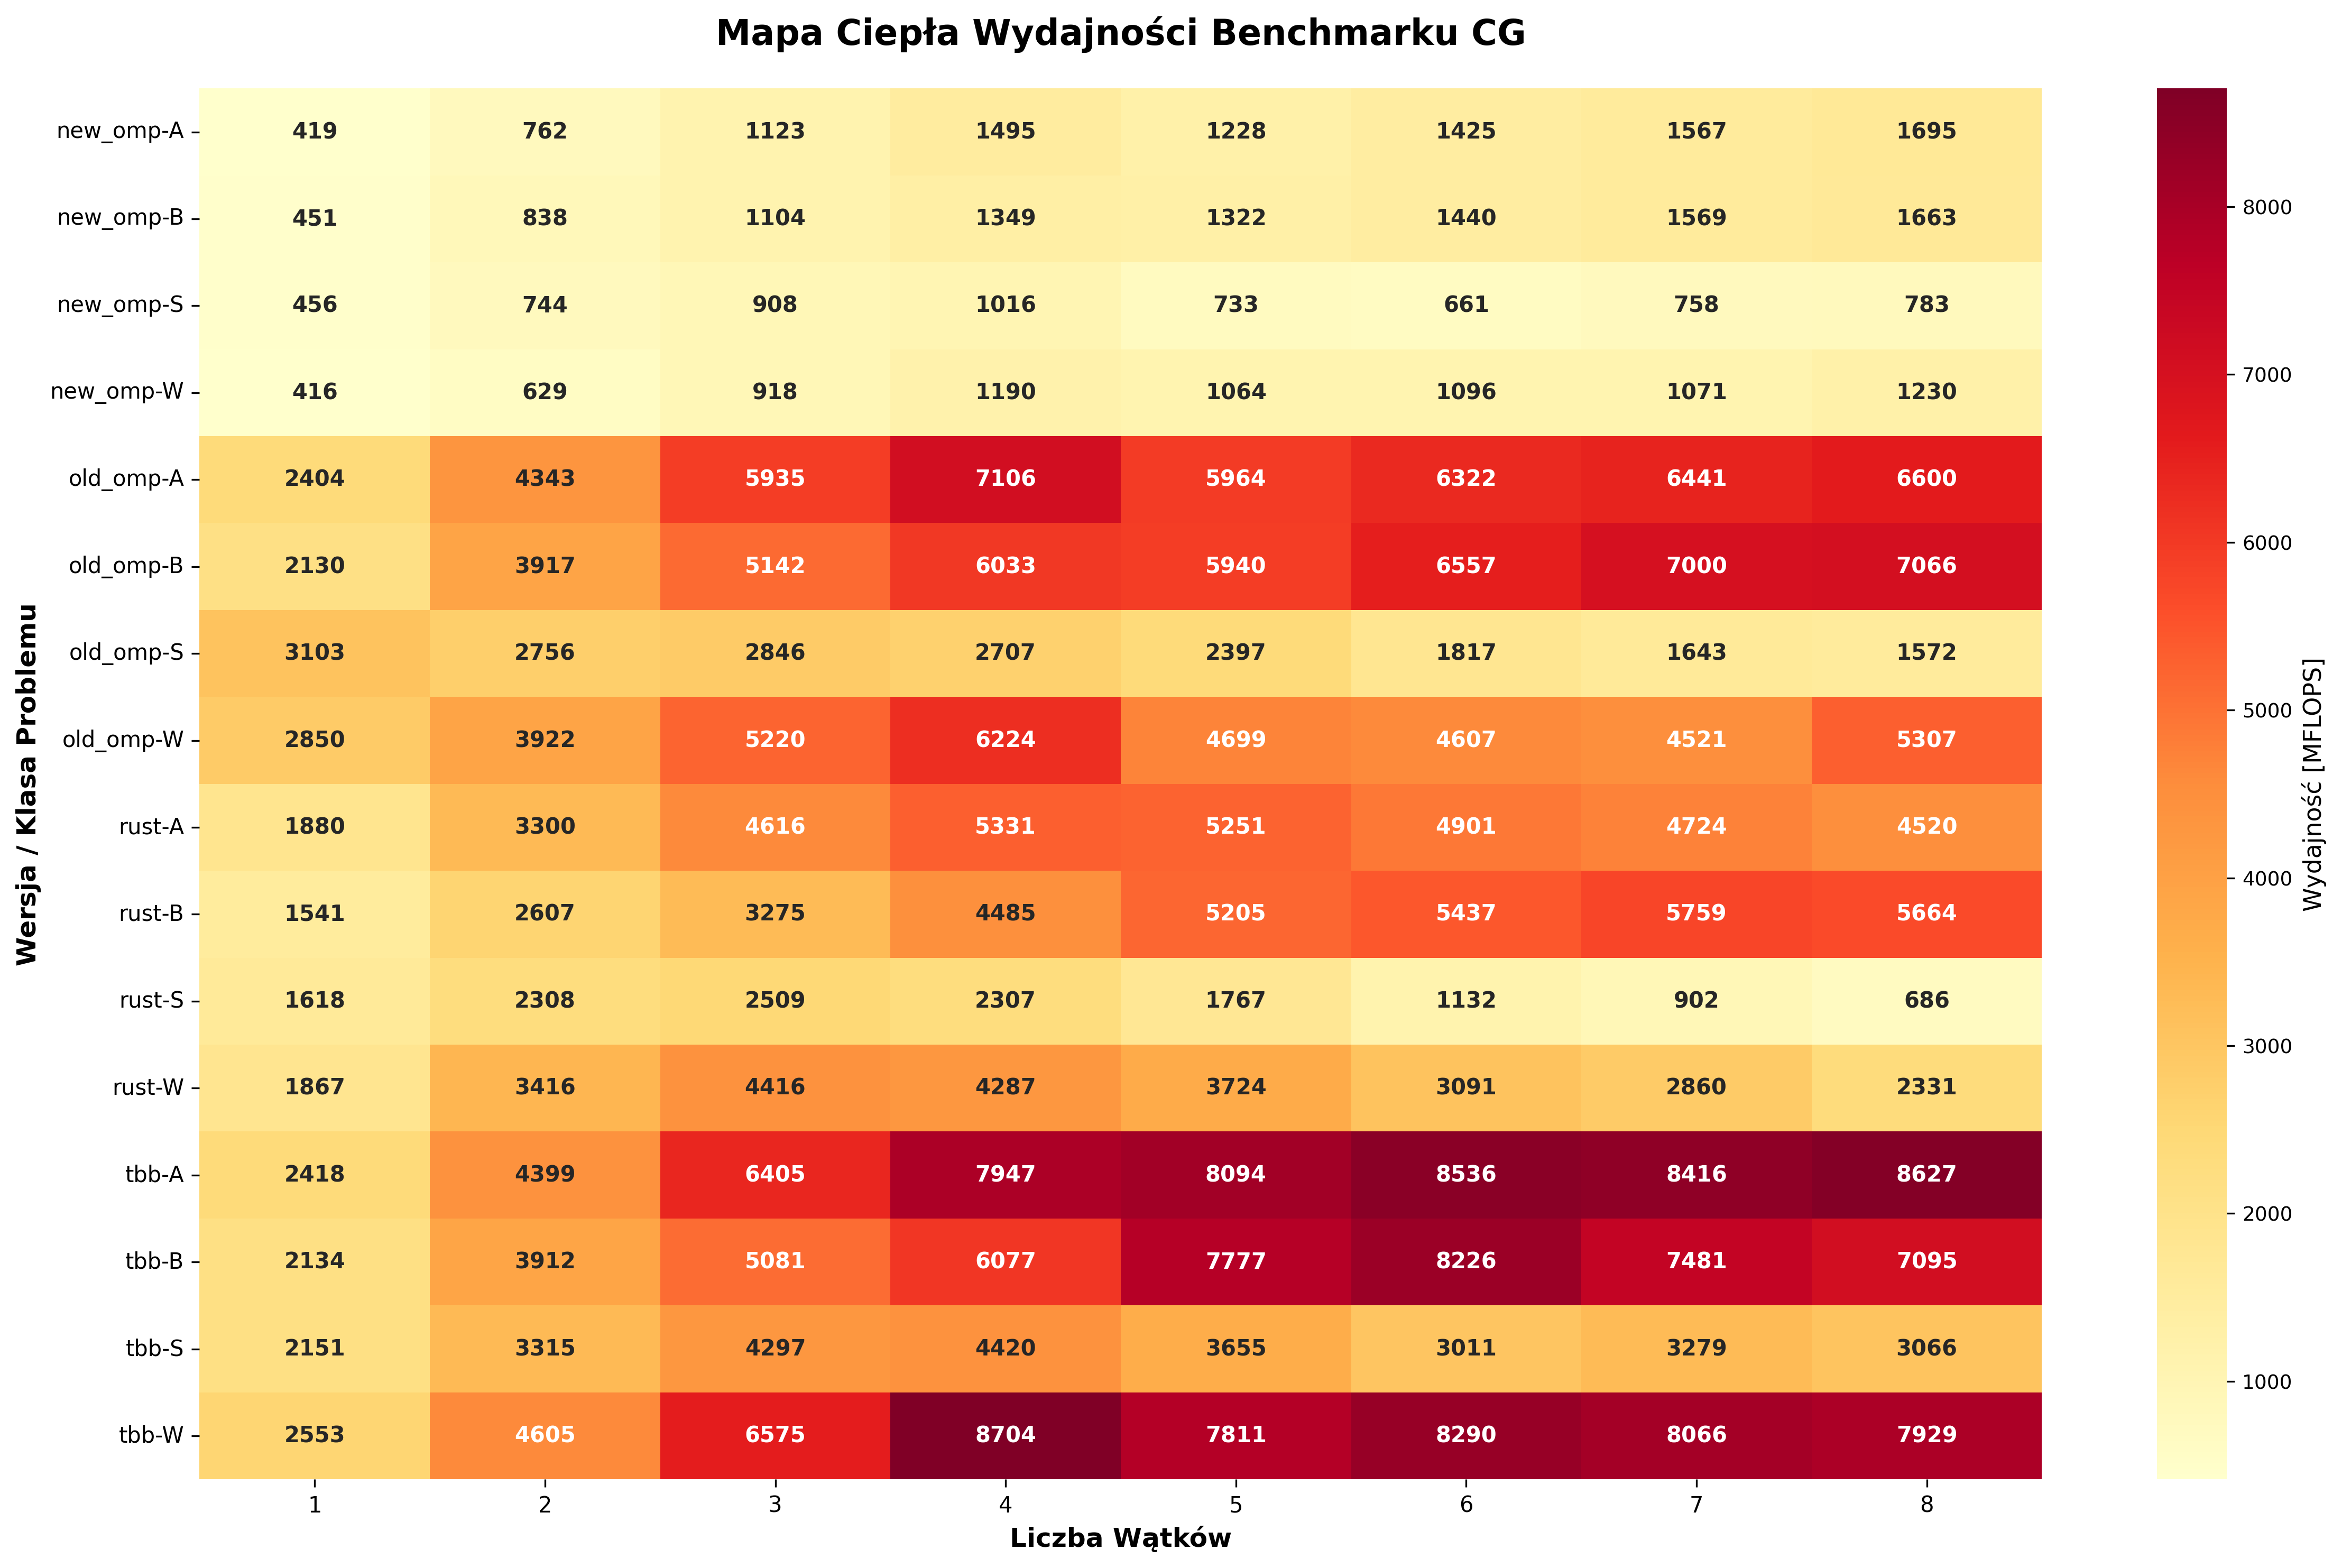
\includegraphics[width=\textwidth]{analiza/images/parallel/cg/arm/cg_mapa_ciepla_wydajnosci.png}
    \caption{Mapa ciepła wydajności benchmarku CG dla klas S, W, A, B względem liczby użytych wątków na platformie ARM64}
    \label{cg_heatmap_wydajnosci}
\end{figure}
Powyższa mapa cieplna - rysunek \ref{cg_heatmap_wydajnosci} przedstawia wydajność (w MFLOPS). Wydajność została przedstawiona w zależności od liczby użytych wątków. Odcienie koloru od żółtego do ciemnoczerwonego wskazują na wzrost wydajności.

\subsubsection{Klasa A}
W klasie A najwyższą wydajność osiąga implementacja tbb, która systematycznie poprawia wyniki aż do 8 wątków, gdzie osiąga wartość 8627 MFLOPS. old\_omp również wykazuje dobre skalowanie, osiągając 6600 MFLOPS przy 8 wątkach. rust oraz new\_omp wypadają wyraźnie słabiej — rust stabilizuje się w przedziale 4500-5300 MFLOPS, natomiast new\_omp osiąga wartość maksymalną około 1700 MFLOPS. Sugeruje to, że tbb oraz old\_omp są znacznie bardziej efektywne w przetwarzaniu większych danych w tej klasie.

\subsubsection{Klasa B}
Dla klasy B, która reprezentuje większy problem obliczeniowy niż klasa A, trendy są podobne. tbb ponownie osiąga najwyższą wydajność (8226 MFLOPS przy 6 wątkach), z niewielkim spadkiem po przekroczeniu tej liczby. old\_omp zachowuje się stabilnie i osiąga porównywalne wartości — do 7066 MFLOPS przy 8 wątkach. rust poprawia wydajność aż do 7 wątków (5759 MFLOPS), po czym następuje niewielki spadek. new\_omp, choć bardziej stabilny, pozostaje najmniej wydajny w tej klasie (maksymalnie 1663 MFLOPS).

\subsubsection{Klasa S}
W przypadku klasy S wyraźnie widoczne są ograniczenia skalowania. tbb i old\_omp osiągają szczytowe wartości przy 3-4 wątkach, po czym wydajność zaczyna spadać. tbb osiąga maksimum (4297 MFLOPS) przy 3 wątkach, natomiast old\_omp przy 2 wątkach (3103 MFLOPS), z wyraźnym trendem malejącym przy dalszym zwiększaniu liczby wątków. rust również notuje spadek po osiągnięciu maksimum (2509 MFLOPS), co może świadczyć o narzuceniu narzutu synchronizacji przy małym rozmiarze danych. new\_omp wypada najsłabiej - spadek wydajności przy większej liczbie wątków sugeruje ograniczoną użyteczność dla tej klasy problemu.

\subsubsection{Klasa W}
Dla klasy W, ponownie najwyższe wartości osiąga tbb, z maksimum 8704 MFLOPS przy 4 wątkach i wysoką stabilnością w dalszych konfiguracjach. old\_omp również prezentuje dobre wyniki, choć maksymalna wydajność (6224 MFLOPS) jest niższa niż w przypadku tbb. Rust osiąga przyzwoite wartości (~5300 MFLOPS przy 8 wątkach), a new\_omp pozostaje konsekwentnie najmniej wydajny (~1200 MFLOPS przy 8 wątkach).


\begin{figure}[H]
    \centering
    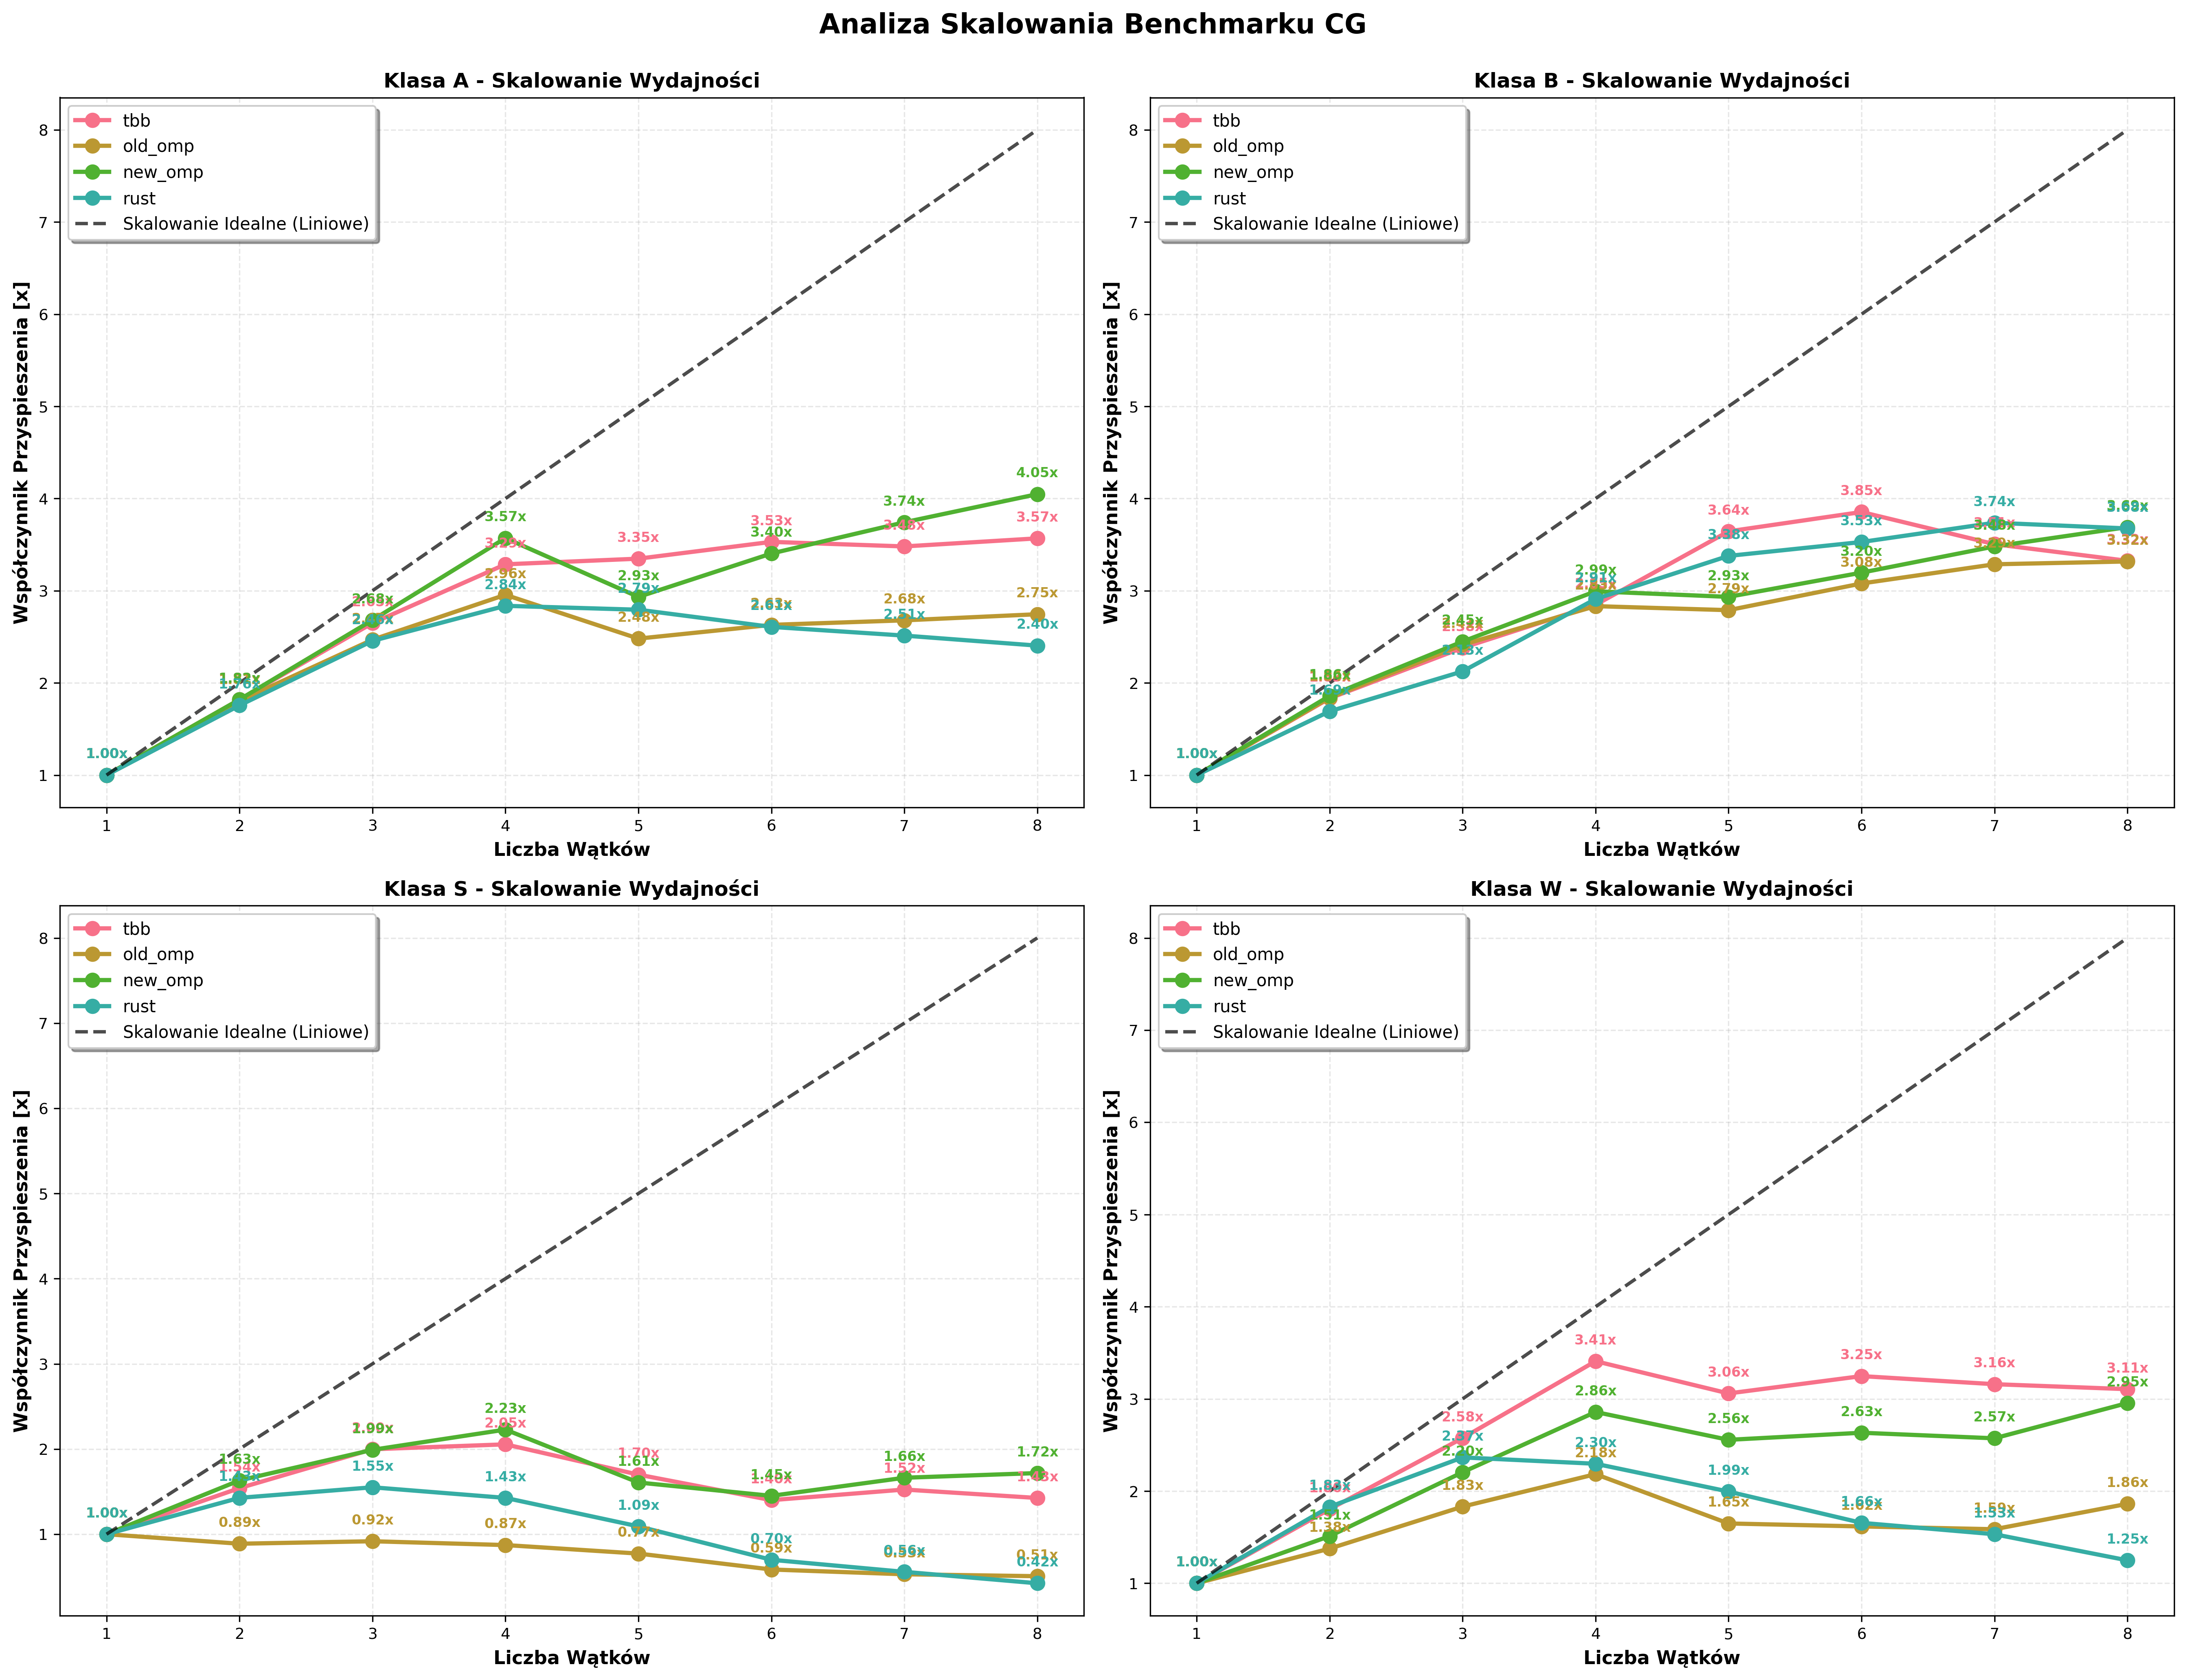
\includegraphics[width=\textwidth]{analiza/images/parallel/cg/arm/cg_analiza_skalowania.png}
    \caption{Analiza skalowania benchmarku CG dla klas S, W, A, B względem liczby użytych wątków na platformie ARM64}
    \label{cg_analiza_skalowania}
\end{figure}
Powyższy wykres - rysunek \ref{cg_analiza_skalowania} przedstawia skalowanie wydajności benchmarku CG. Skalowanie wyrażone zostało za pomocą współczynnika przyspieszenia względem wykonania jednowątkowego i odniesione do skalowania idealnego (liniowego).

Analiza wykresów ujawnia wyraźne różnice w charakterystyce skalowalności pomiędzy implementacjami. W przypadku większych klas problemów (A, B, W) implementacje tbb oraz rust wykazują najbardziej efektywne skalowanie, osiągając współczynniki przyspieszenia przekraczające 3x przy 8 wątkach, z lokalnymi maksimami już przy 4-6 wątkach. Choć żaden z wariantów nie osiąga idealnego skalowania liniowego, to tbb zbliża się do tego poziomu najbliżej, szczególnie w klasach A i B.

Implementacja old\_omp wykazuje umiarkowane skalowanie, a jej przyspieszenie rośnie wraz z liczbą wątków, jednak wolniej niż w przypadku tbb czy rust. Współczynniki przyspieszenia dla old\_omp są stabilne, ale znacznie oddalone od linii idealnej, co może wskazywać na ograniczenia w zarządzaniu wątkami i efektywności synchronizacji.

new\_omp prezentuje wyraźnie najniższe wartości przyspieszenia we wszystkich klasach problemu. Współczynnik dla tej implementacji często osiąga maksimum przy 2-4 wątkach, po czym jego wzrost ulega zahamowaniu lub wręcz obserwowany jest spadek. Taki przebieg może świadczyć o niskiej efektywności skalowania wynikającej z narzutu synchronizacji, nieefektywnej dekompozycji zadań lub nieadekwatnego wykorzystania zasobów systemowych w przypadku większej liczby wątków.

Zwraca uwagę, że klasy problemu o większym rozmiarze (B i W) wykazują generalnie lepsze skalowanie niż klasy mniejsze (S), co jest zgodne z teoretycznym założeniem, że większy problem obliczeniowy lepiej amortyzuje koszty narzutów komunikacyjnych i synchronizacyjnych. W klasie S przyrost przyspieszenia jest niewielki lub wręcz ujemny dla niektórych implementacji, co wskazuje na zbyt małą ilość pracy do równomiernego rozproszenia pomiędzy rdzenie procesora.


\subsection{Wyniki benchmarków - platforma x86\_64}
\begin{figure}[H]
    \centering
    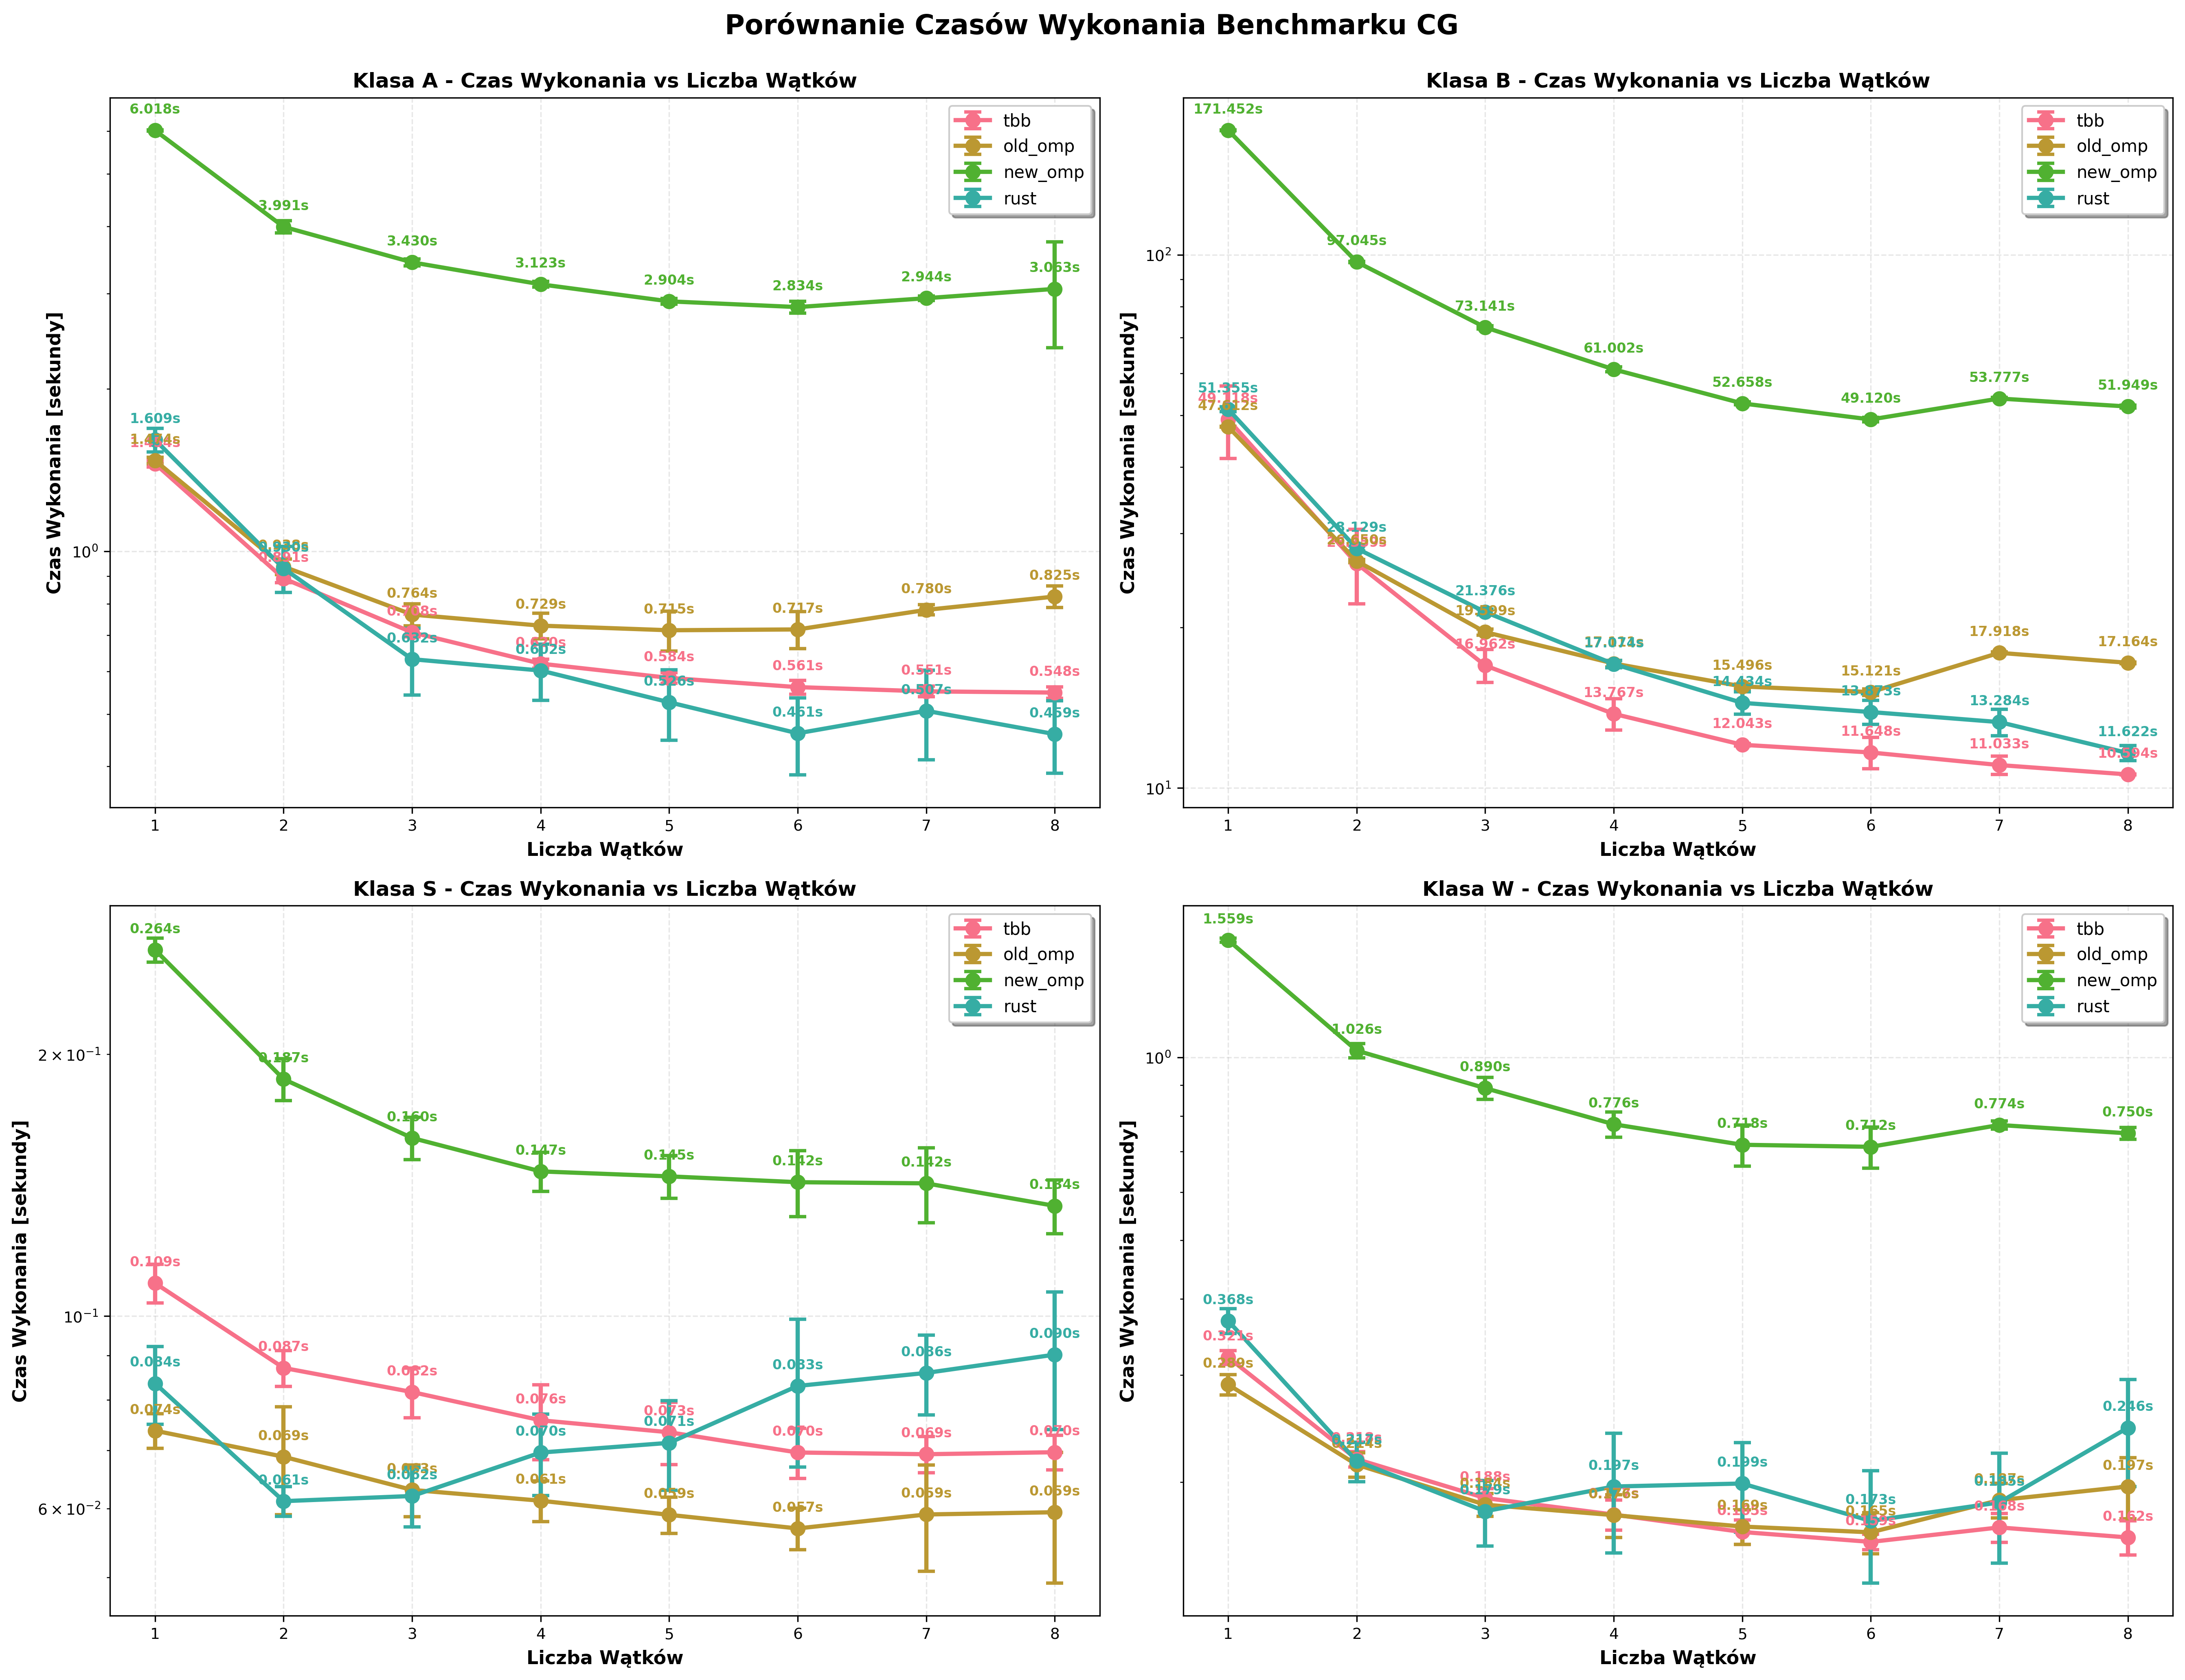
\includegraphics[width=\textwidth]{analiza/images/parallel/cg/x86/cg_porownanie_czasow_wykonania.png}
    \caption{Porównanie czasów wykonania benchmarku CG dla klas S, W, A, B względem liczby użytych wątków na platformie x86\_64}
    \label{cg_porownanie_czasow_wykonania_x86_64}
\end{figure}


\begin{figure}[H]
    \centering
    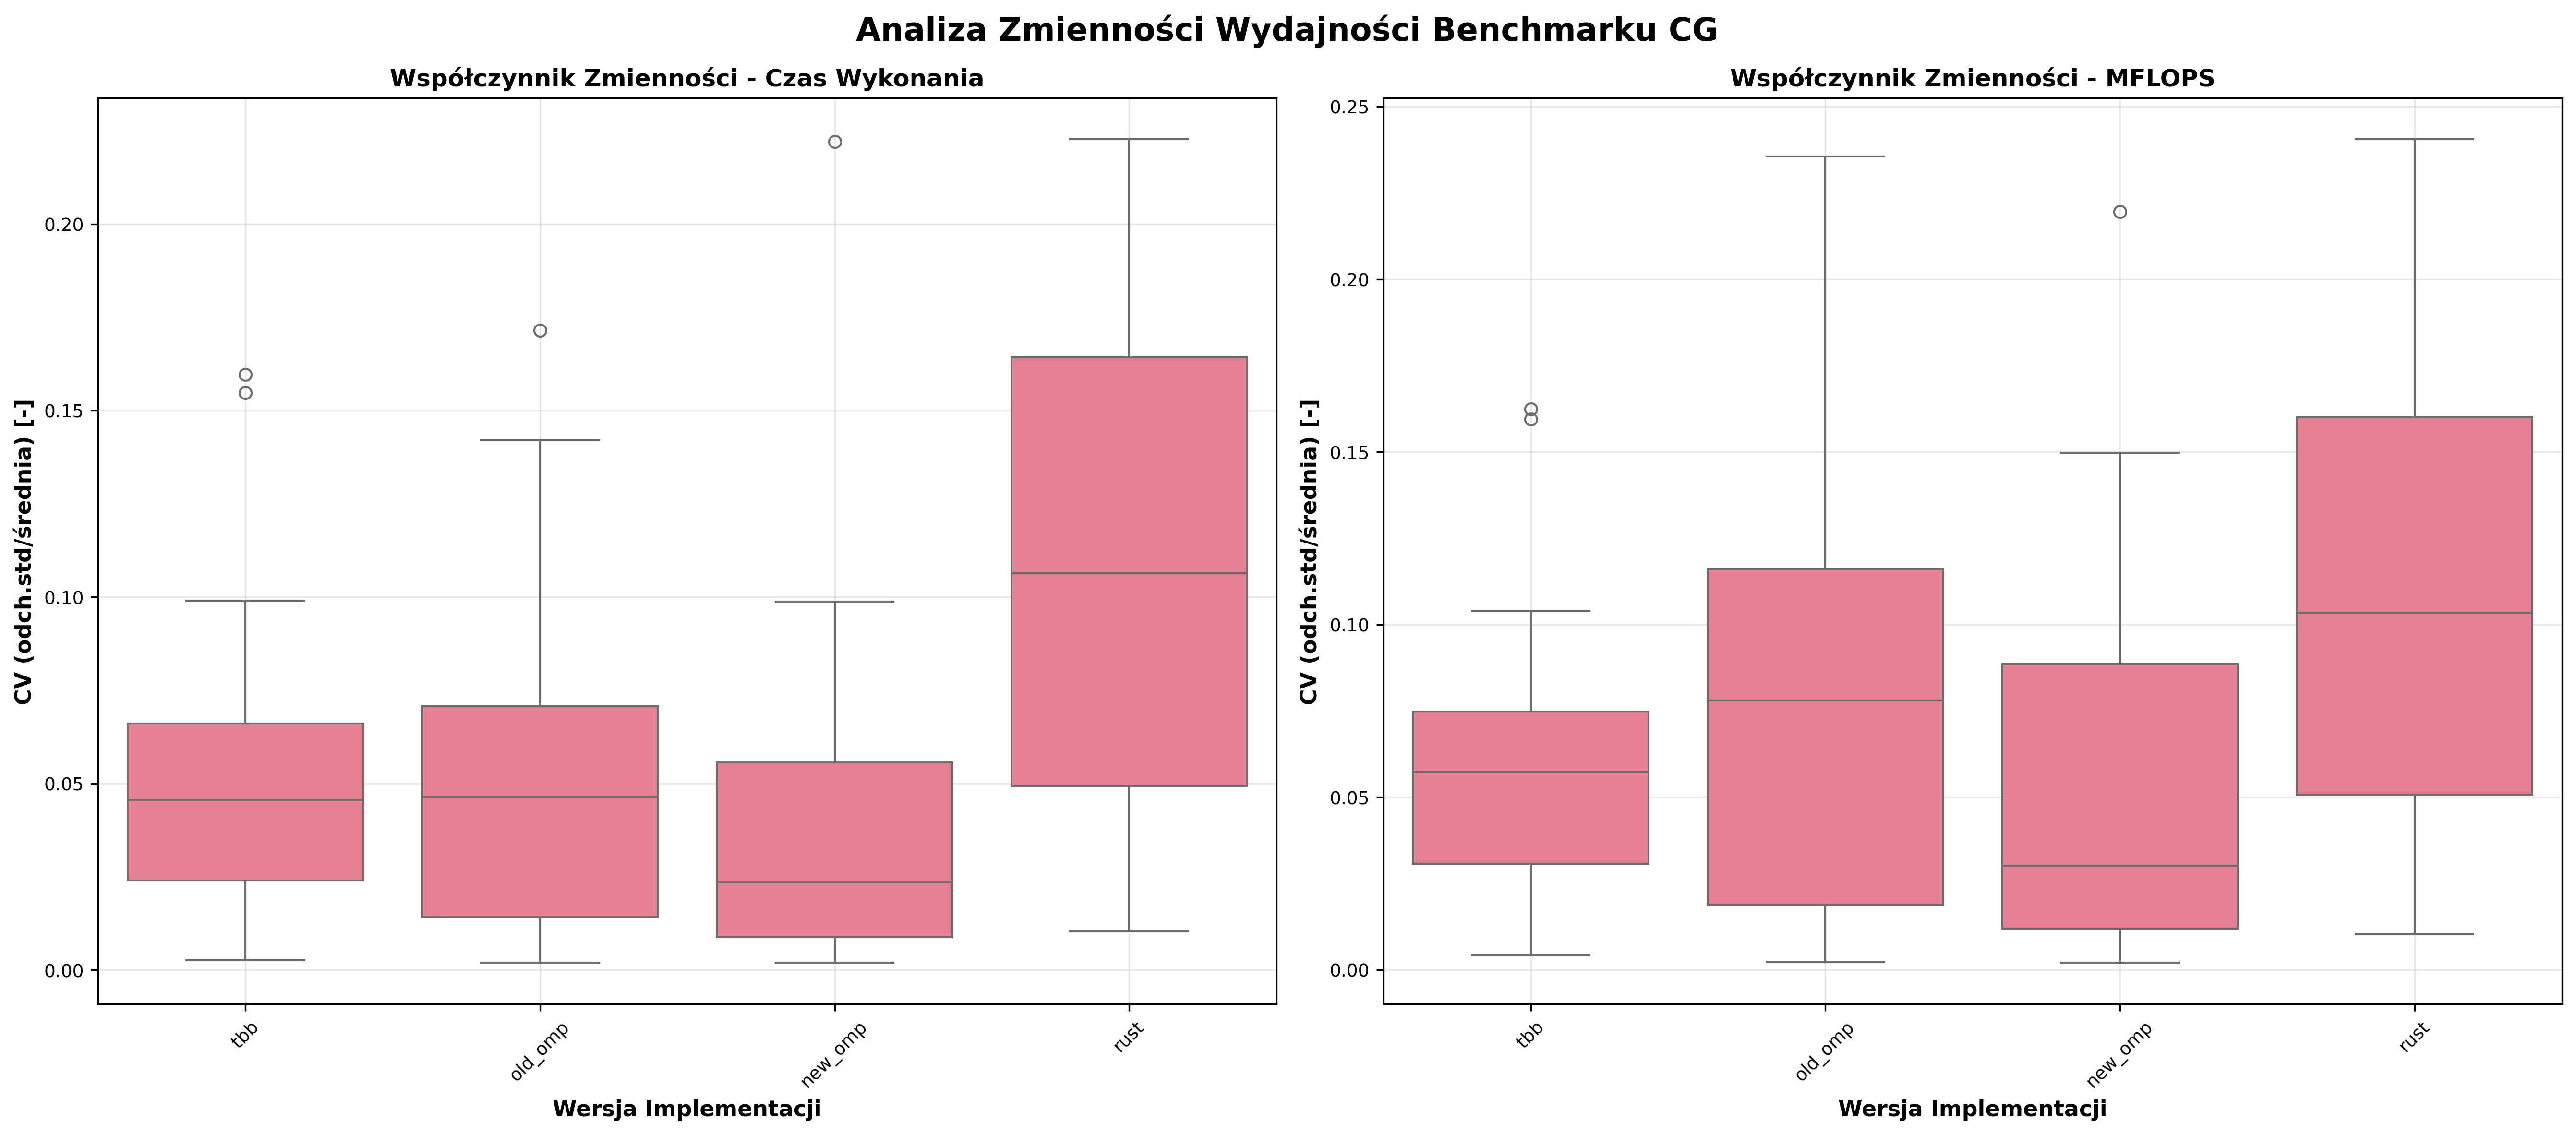
\includegraphics[width=\textwidth]{analiza/images/parallel/cg/x86/cg_analiza_zmiennosci.png}
    \caption{Analiza zmienności czasów wykonania benchmarku CG dla klas S, W, A, B względem liczby użytych wątków na platformie x86\_64}
    \label{cg_analiza_zmiennosci_x86_64}
\end{figure}
Wykresy - rysunek \ref{cg_porownanie_czasow_wykonania_x86_64} przedstawiają czasy wykonania benchmarku CG dla czterech klas problemu (A, B, S, W) w zależności od liczby wątków, dla czterech implementacji równoległych: tbb, old\_omp, new\_omp i rust.

Implementacje TBB oraz new\_omp wykazują istotne skrócenie czasu wykonania wraz ze wzrostem liczby wątków, zwłaszcza w przypadku klas A, B oraz W.

Z kolei old\_omp charakteryzuje się umiarkowaną poprawą czasu wykonania; jednak w konfiguracjach z większą liczbą wątków, szczególnie dla klasy B, obserwuje się wyraźne pogorszenie wyników. Może to wskazywać na istotny narzut związany z synchronizacją lub nieefektywny podział pracy między wątki.

Implementacja w języku Rust, mimo że w niektórych przypadkach osiąga zadowalające rezultaty przy mniejszej liczbie wątków, traci tę przewagę w miarę zwiększania równoległości. Może to być konsekwencją ograniczeń w mechanizmach zarządzania wielowątkowością lub niedostosowanej strategii dekompozycji zadań.

W przypadku klasy S, reprezentującej niewielki problem obliczeniowy, wszystkie analizowane implementacje osiągają bardzo krótkie czasy wykonania. Wzrost liczby wątków przynosi w tym przypadku jedynie marginalne korzyści, a w niektórych przypadkach prowadzi wręcz do spadku wydajności, co można tłumaczyć narzutem wynikającym z równoleglenia w stosunku do niewielkiej skali problemu.

Z analizy rozkładu - rysunek \ref{cg_analiza_zmiennosci_x86_64} zmienności wynika, że implementacja new\_omp cechuje się najniższą zmiennością zarówno w zakresie czasu wykonania, jak i osiąganej wydajności (mierzonej w MFLOPS). Świadczy to o wysokim stopniu przewidywalności oraz deterministycznym charakterze działania tej wersji, mimo jej ogólnie niższej efektywności obliczeniowej.

Implementacje TBB oraz old\_omp wykazują umiarkowaną zmienność wyników. W ich przypadku zaobserwowano pojedyncze wartości odstające, szczególnie w przypadku TBB, co może wskazywać na niekonsystentne zachowanie w określonych warunkach wykonawczych, takich jak zwiększone obciążenie systemu lub interferencje z innymi procesami.

Z kolei implementacja w języku Rust, mimo że w wybranych przypadkach oferowała dobre rezultaty czasowe, charakteryzuje się najwyższą zmiennością spośród analizowanych rozwiązań. Wysoka wariancja obserwowana w różnych konfiguracjach eksperymentalnych może świadczyć o ograniczonej stabilności tej implementacji, bądź środowiska wykonawczego, w którym została uruchomiona.

\begin{figure}[H]
    \centering
    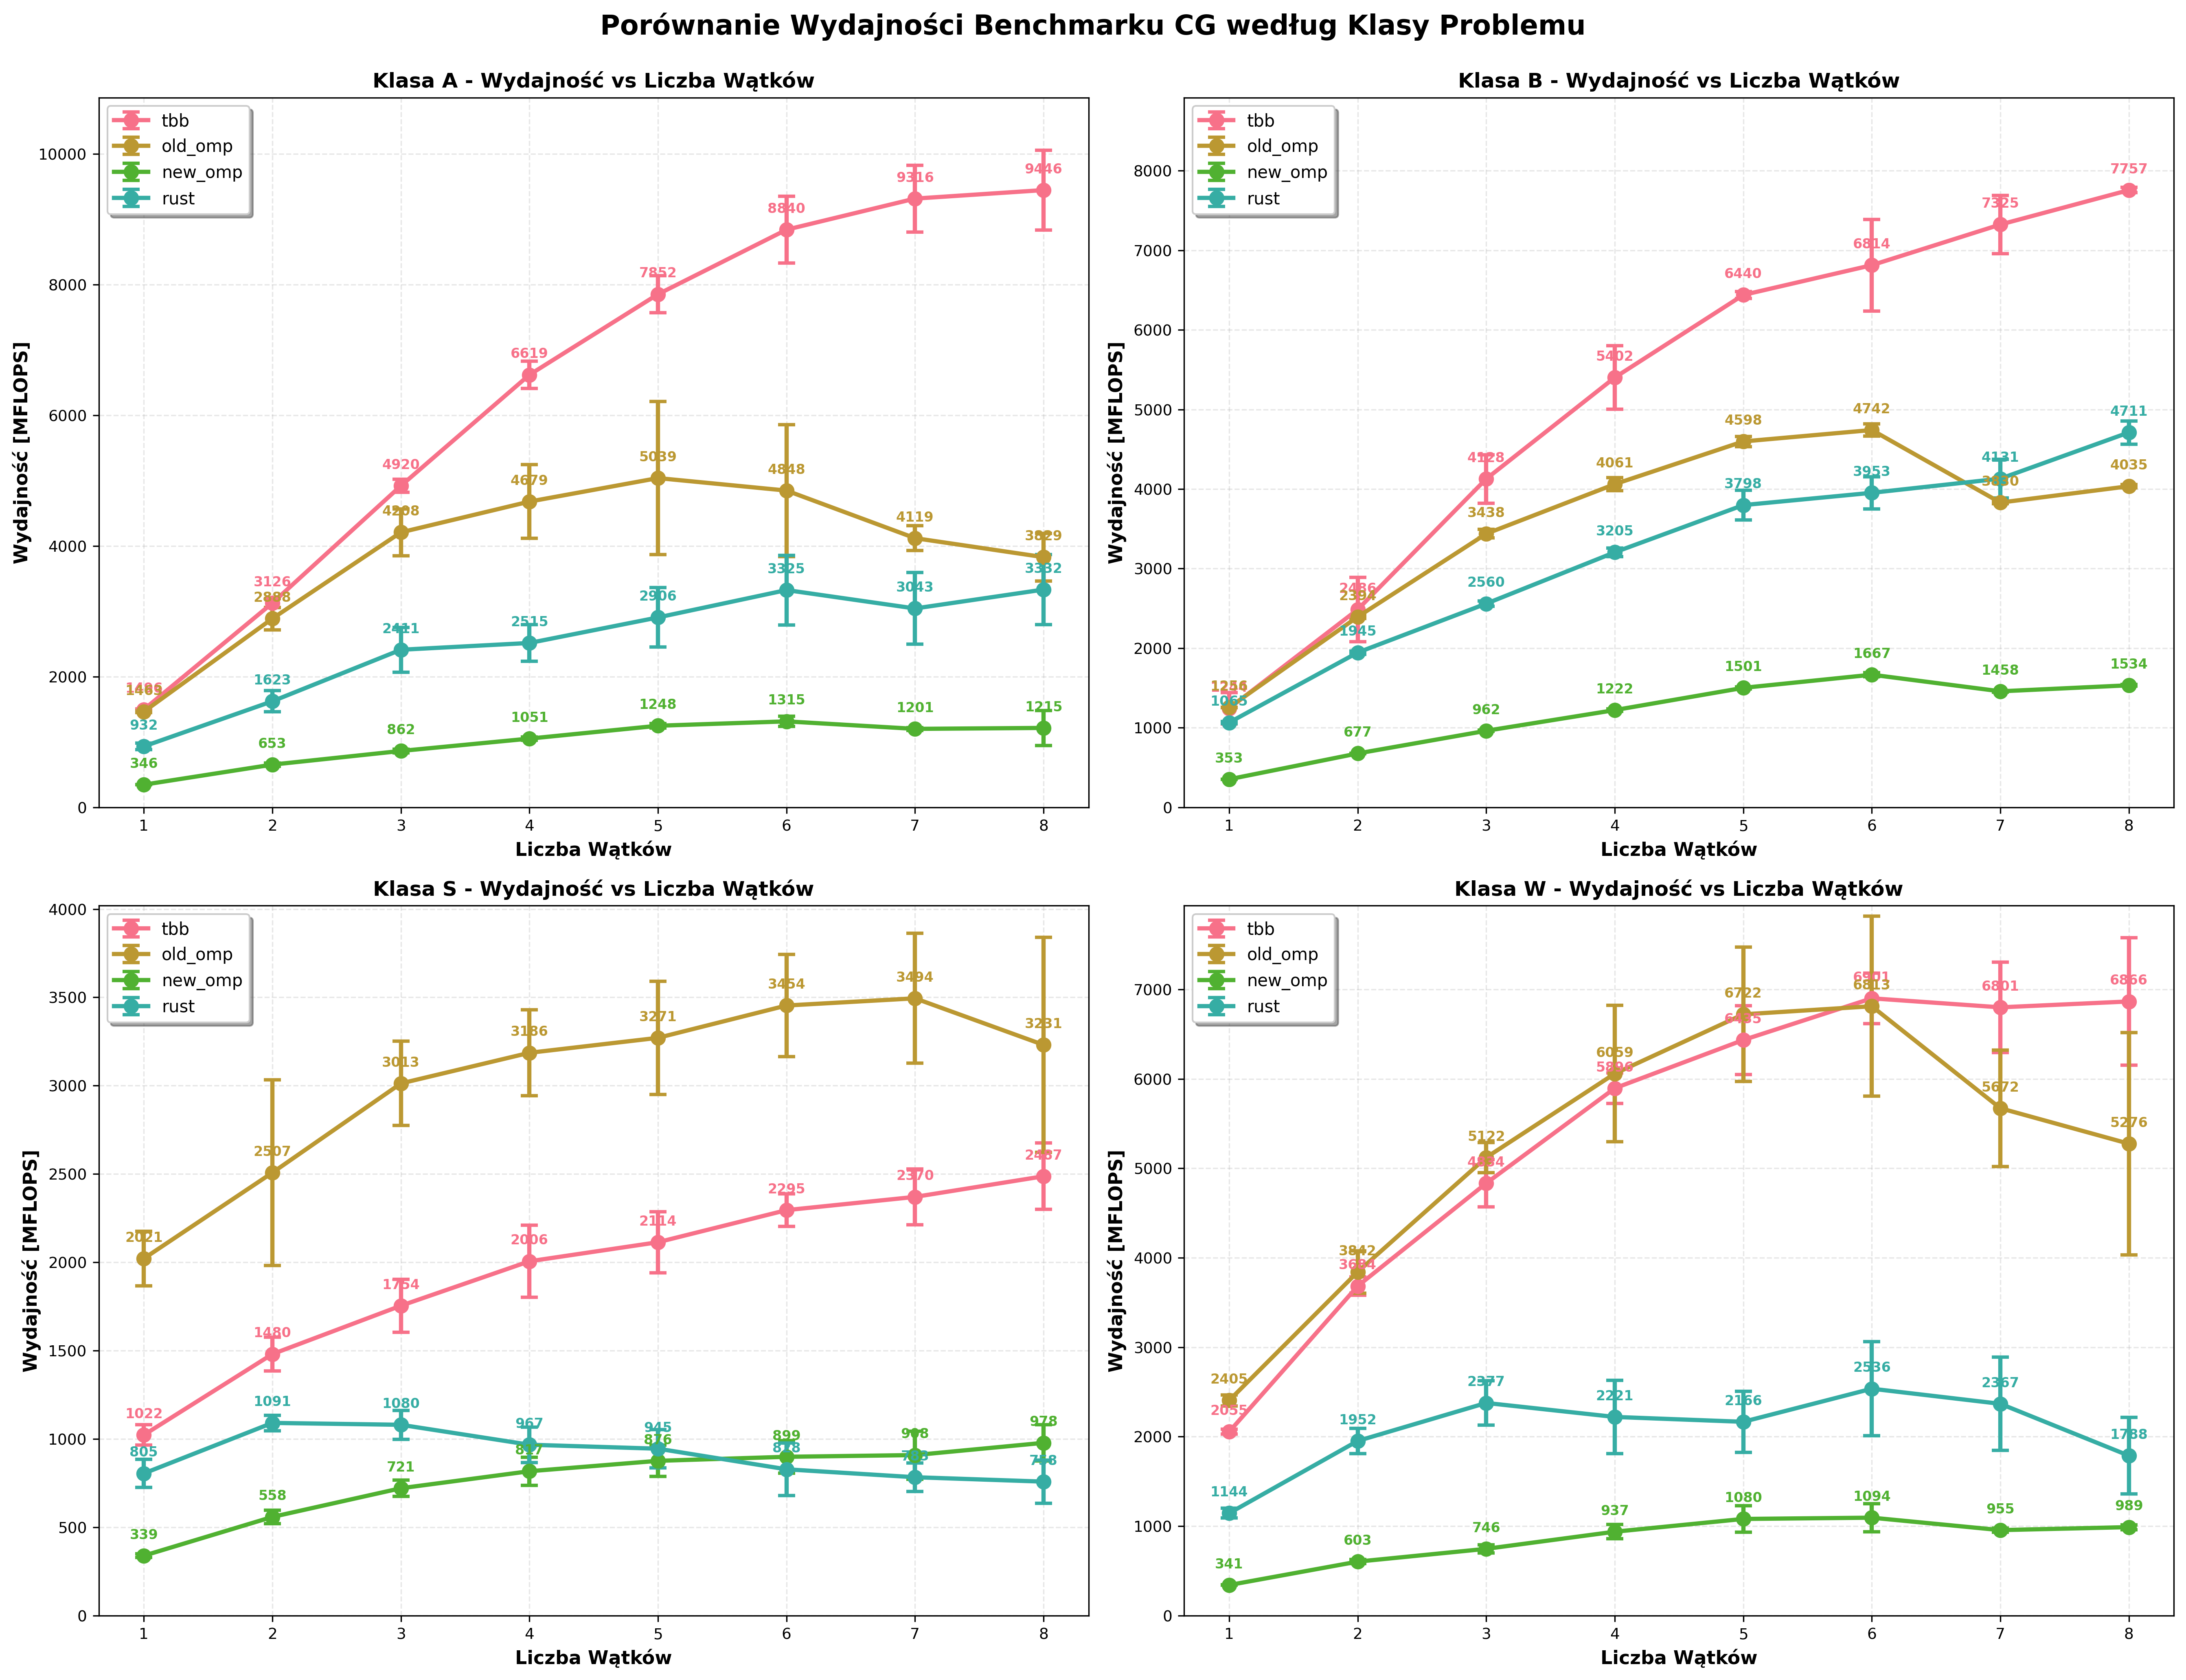
\includegraphics[width=\textwidth]{analiza/images/parallel/cg/x86/cg_porownanie_wydajnosci.png}
    \caption{Porównanie wydajności benchmarku CG dla klas S, W, A, B względem liczby użytych wątków na platformie ARM64}
    \label{cg_porownanie_wydajnosci_x86_64}
\end{figure}
Na wykresach na rysunku \ref{cg_porownanie_wydajnosci_x86_64} zaprezentowano porównanie wydajności benchmarku CG mierzonej w MFLOPS (milionach operacji zmiennoprzecinkowych na sekundę). Wydajność została przedstawiona jako funkcja liczby wątków (1-8) dla czterech implementacji równoległych.

\begin{figure}[H]
    \centering
    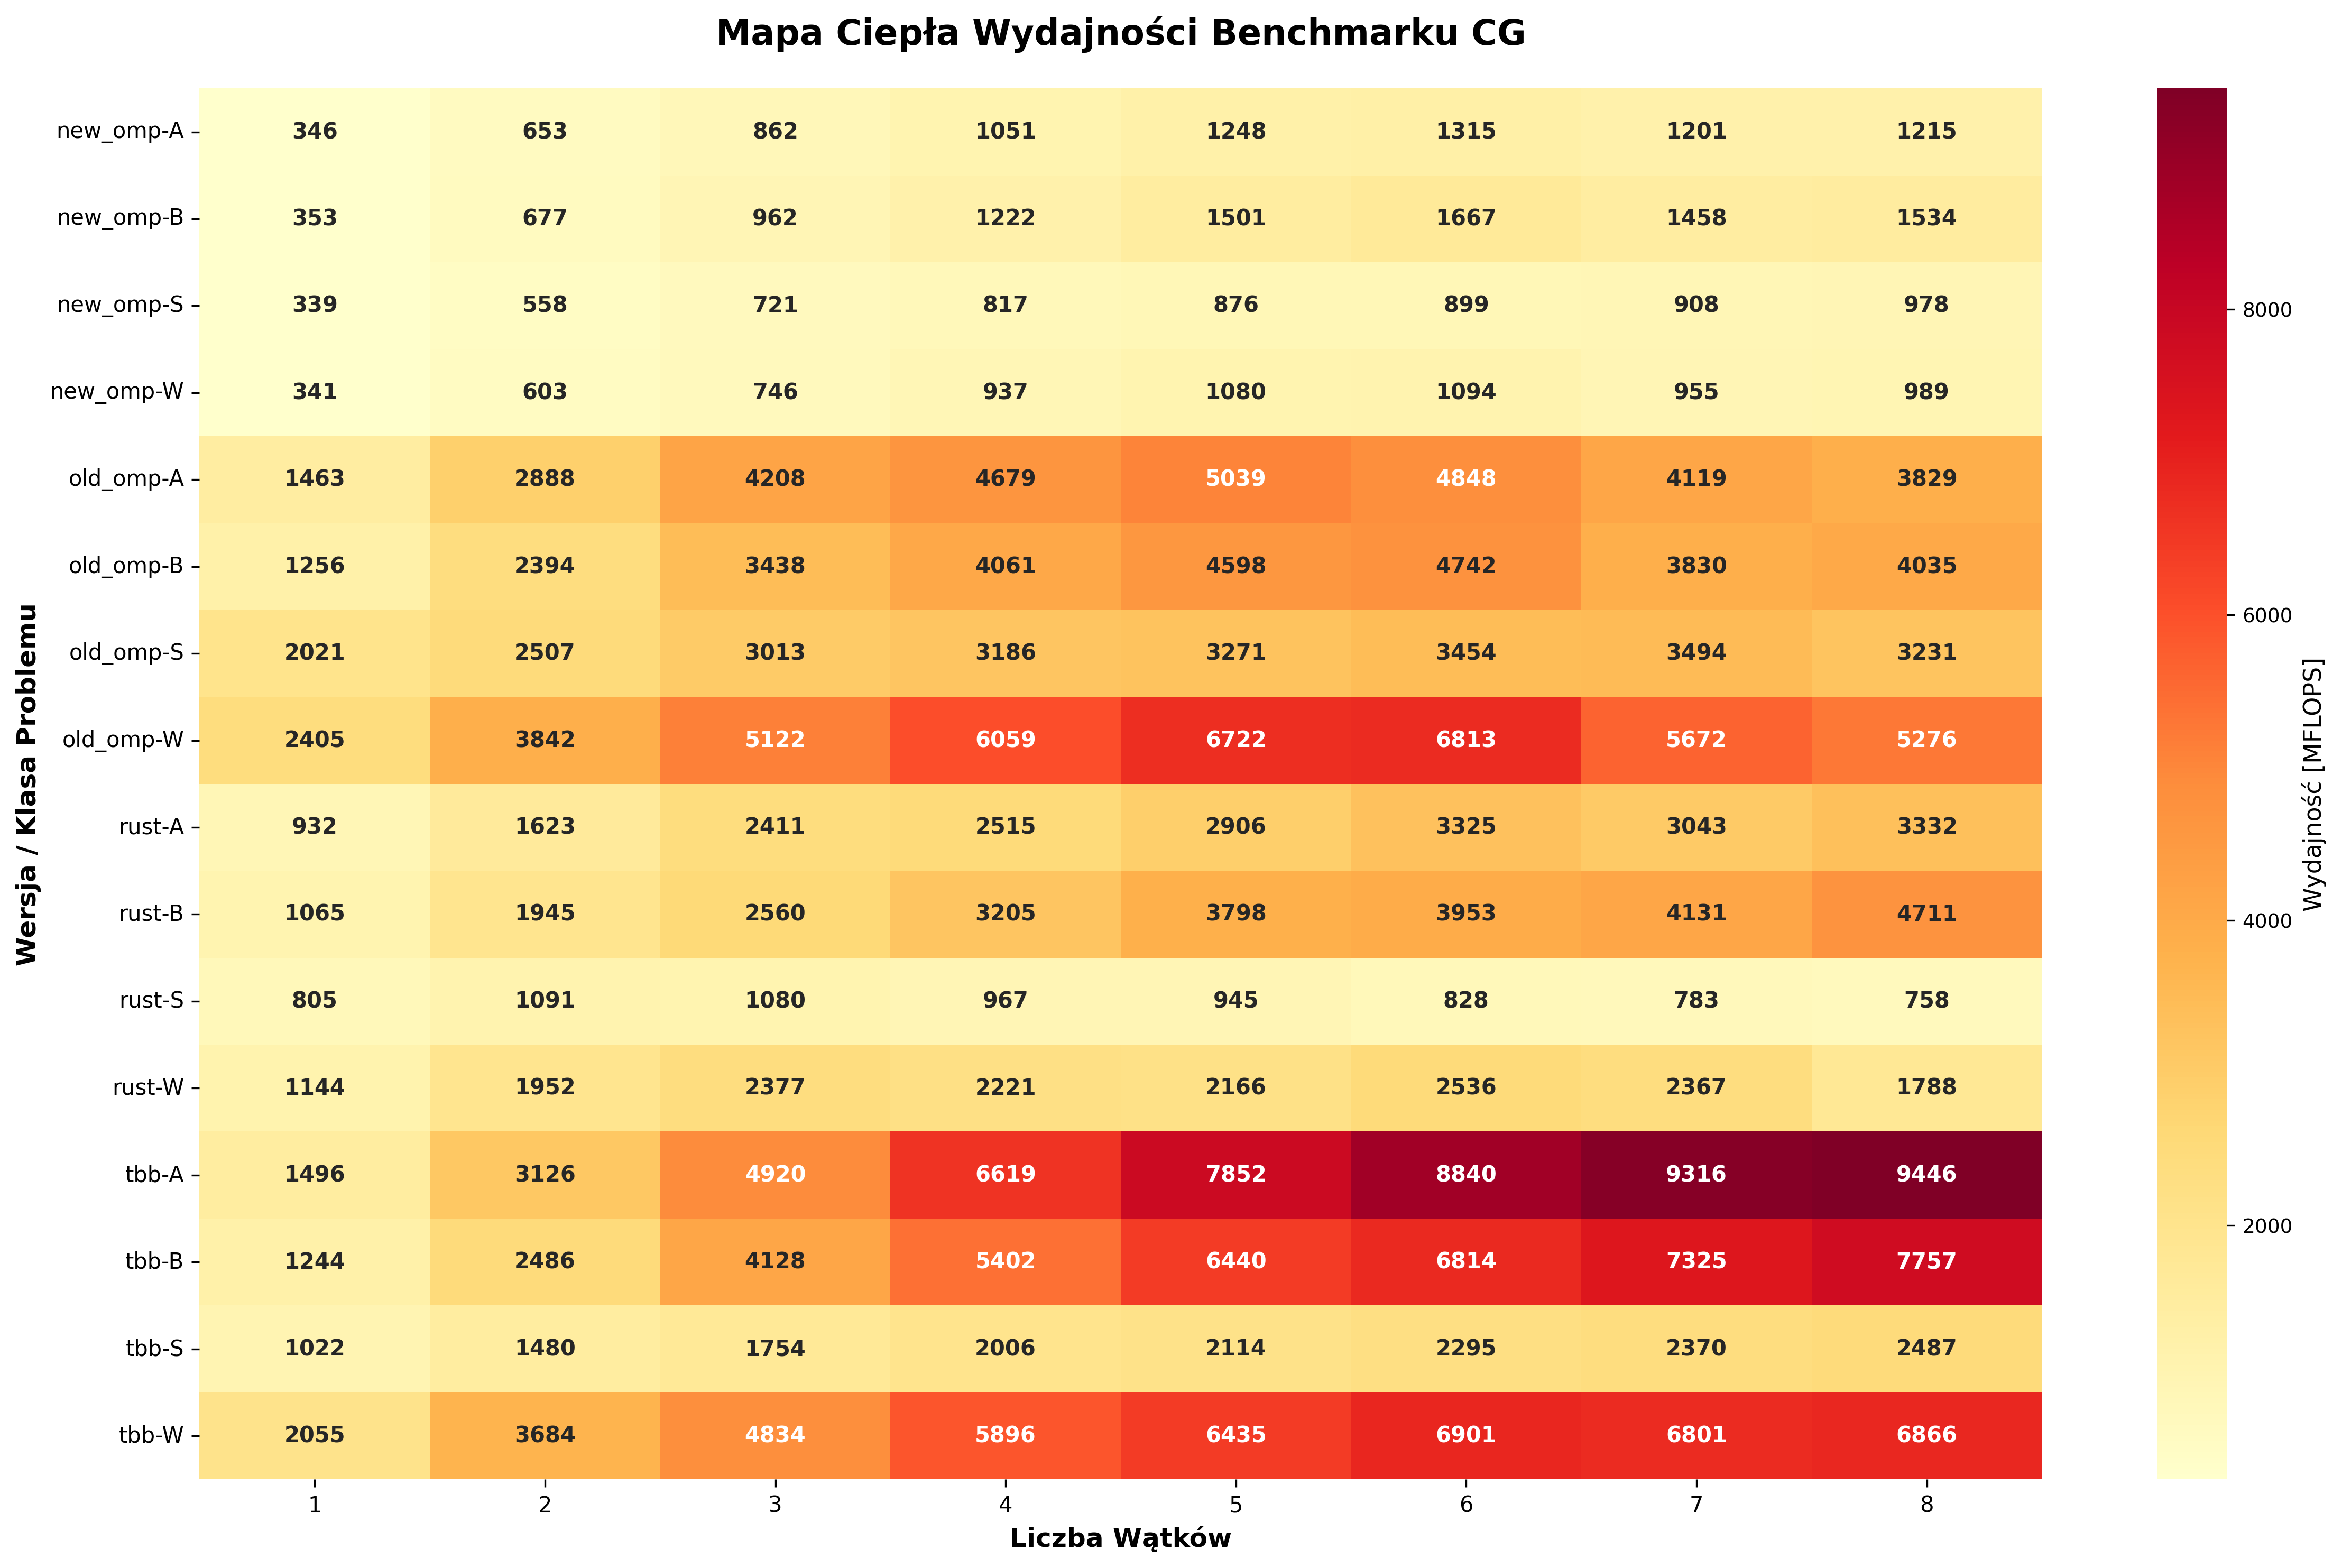
\includegraphics[width=\textwidth]{analiza/images/parallel/cg/x86/cg_mapa_ciepla_wydajnosci.png}
    \caption{Mapa ciepła wydajności benchmarku CG dla klas S, W, A, B względem liczby użytych wątków na platformie ARM64}
    \label{cg_heatmap_wydajnosci_x86_64}
\end{figure}
Powyższa mapa cieplna - rysunek \ref{cg_heatmap_wydajnosci_x86_64} przedstawia wydajność (w MFLOPS). Wydajność została przedstawiona w zależności od liczby użytych wątków. Odcienie koloru od żółtego do ciemnoczerwonego wskazują na wzrost wydajności.

Implementacja tbb wyraźnie dominuje we wszystkich klasach problemu, wykazując największy przyrost wydajności wraz ze wzrostem liczby wątków. W klasie A osiąga wartość bliską 9500 MFLOPS przy 8 wątkach, a w klasie B niemal 7800 MFLOPS. Również w klasach W i S tbb prezentuje bardzo dobre rezultaty, konsekwentnie przewyższając pozostałe implementacje.

old\_omp zajmuje drugą pozycję pod względem wydajności. Choć w klasach A i B nie osiąga wyników tbb, to w klasach W i S oferuje konkurencyjne rezultaty. W szczególności w klasie S przy mniejszej liczbie wątków (2-4) uzyskuje najwyższe wartości MFLOPS w porównaniu z pozostałymi implementacjami, co sugeruje jego efektywność dla mniejszych problemów obliczeniowych.

Rust wykazuje umiarkowaną wydajność, która rośnie do pewnego momentu (najczęściej przy 5-6 wątkach), po czym następuje stabilizacja lub nawet lekki spadek.

Najniższe wyniki uzyskuje new\_omp, którego krzywe wzrostu MFLOPS są płaskie i znacznie oddalone od pozostałych implementacji. Nawet przy większej liczbie wątków nie obserwuje się znaczącej poprawy wydajności.

\begin{figure}[H]
    \centering
    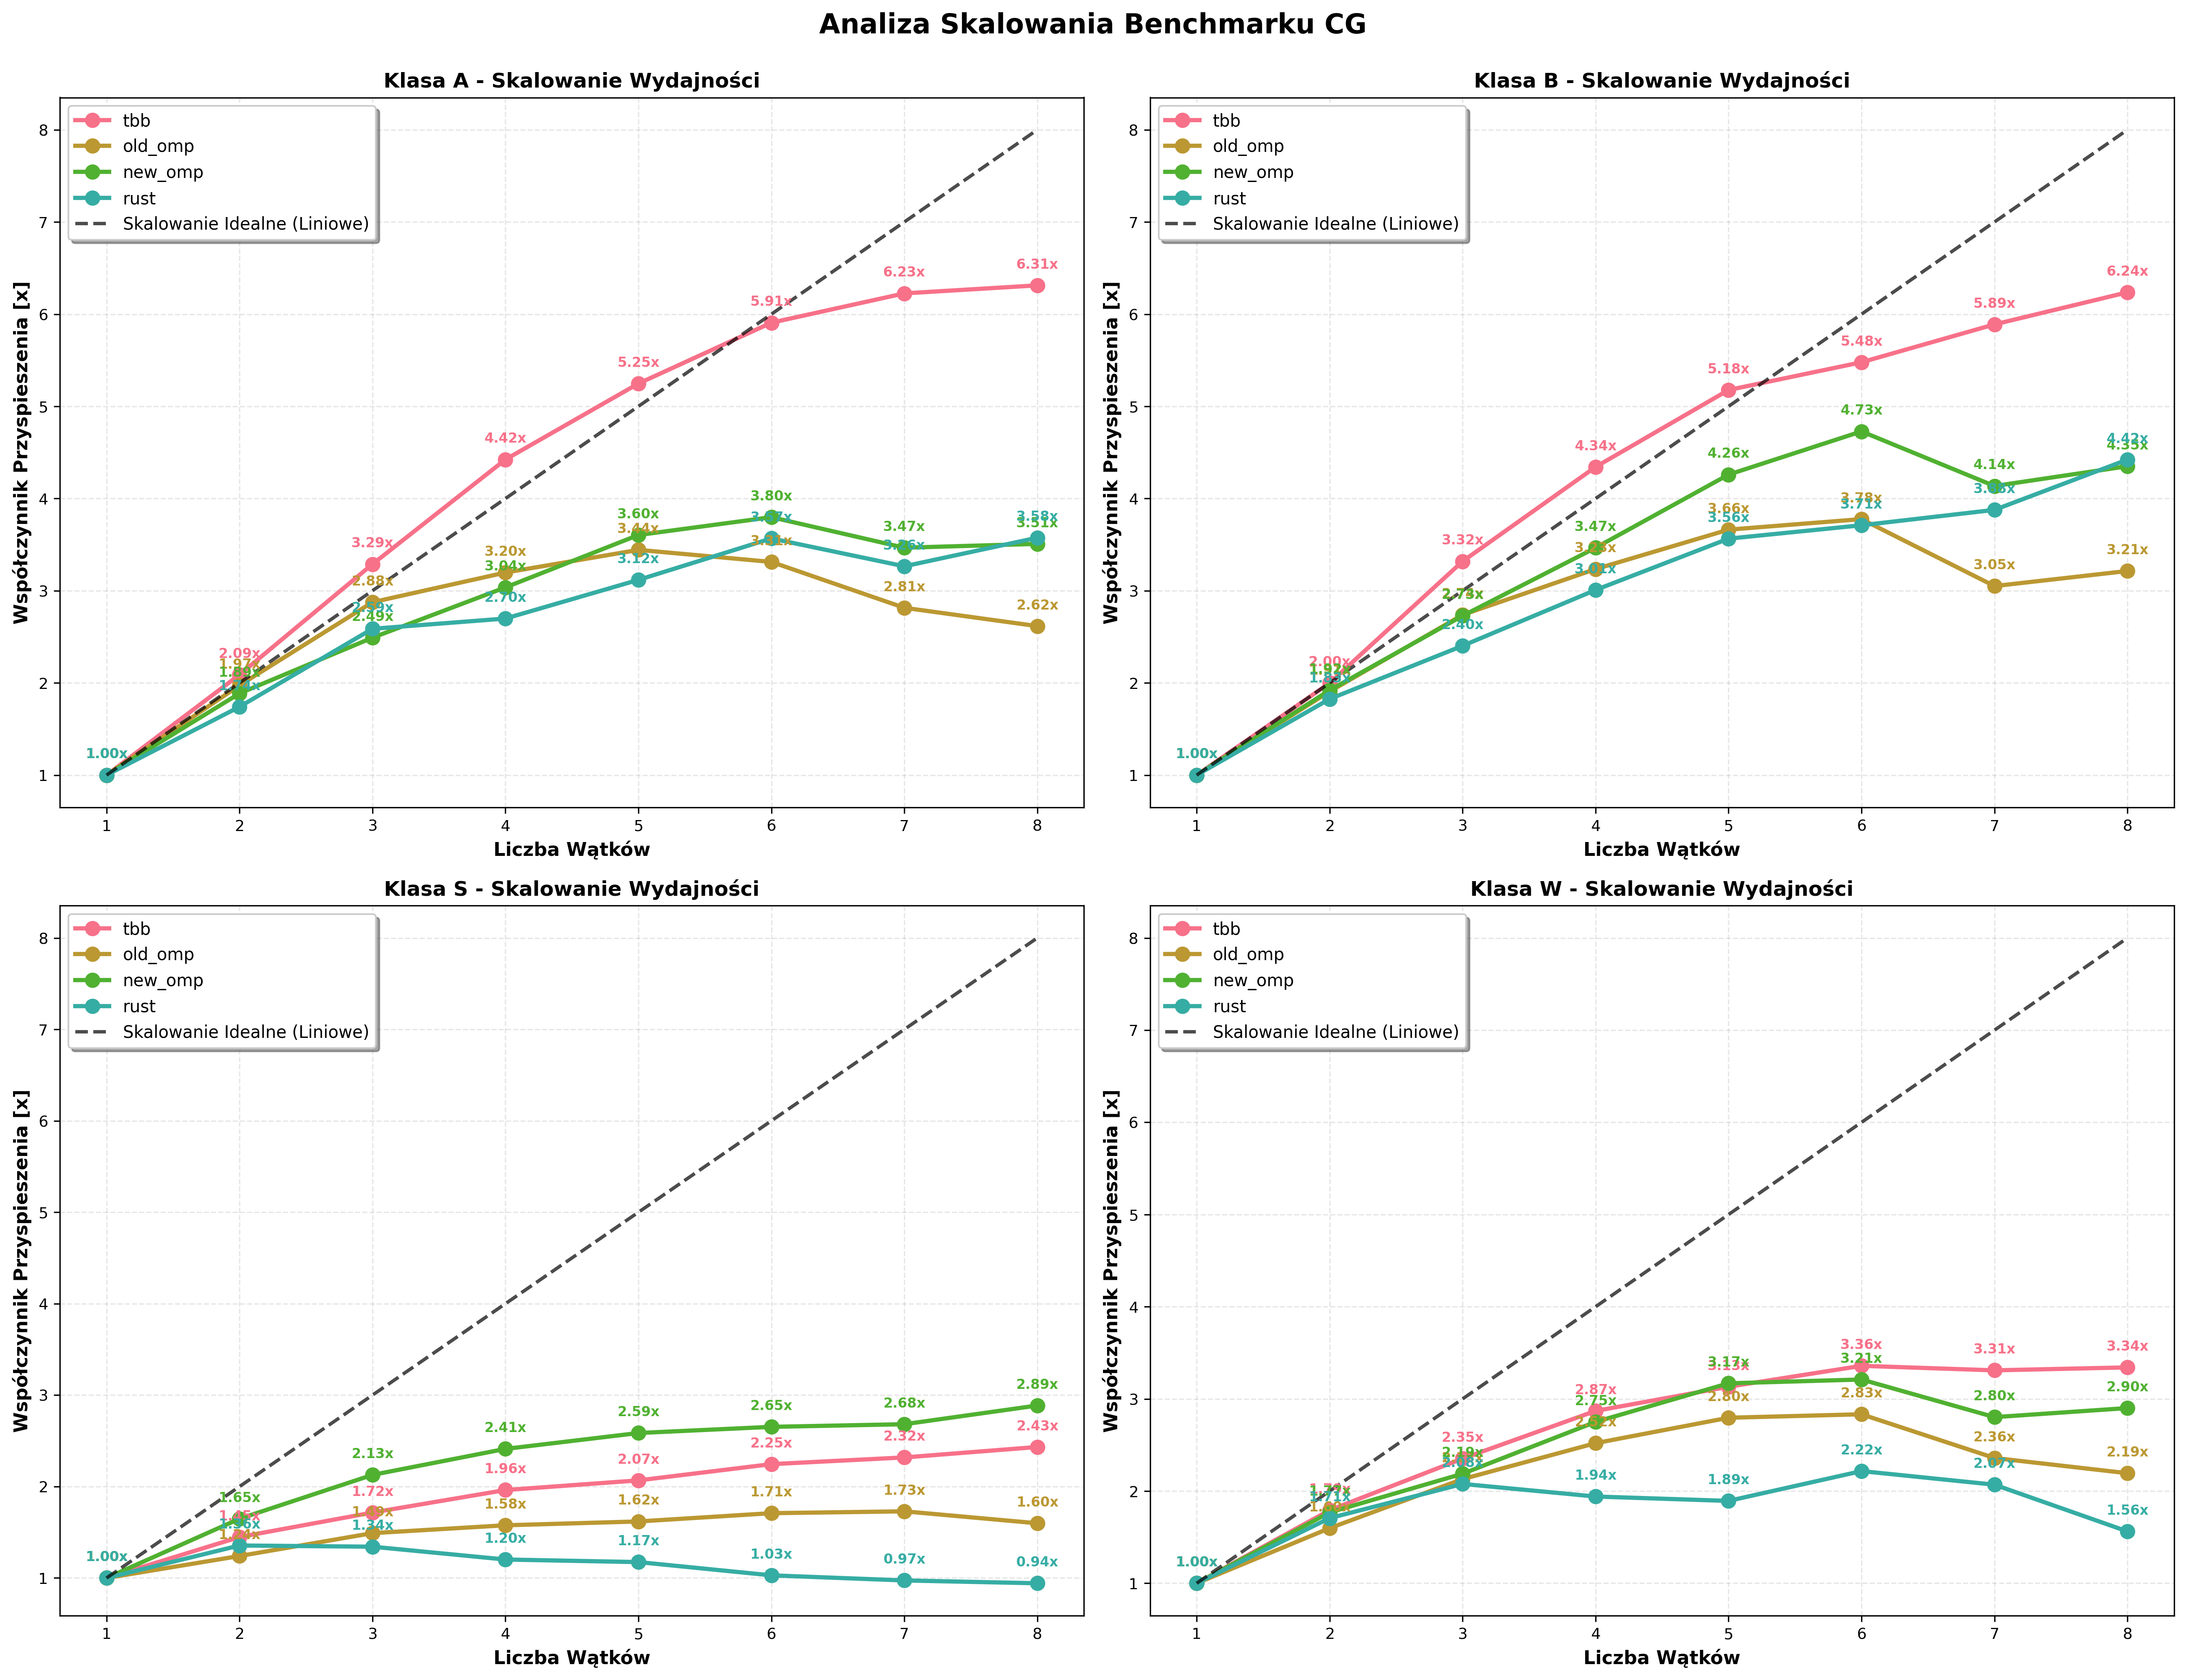
\includegraphics[width=\textwidth]{analiza/images/parallel/cg/x86/cg_analiza_skalowania.png}
    \caption{Analiza skalowania benchmarku CG dla klas S, W, A, B względem liczby użytych wątków na platformie ARM64}
    \label{cg_analiza_skalowania_x86_64}
\end{figure}
Powyższy wykres - rysunek \ref{cg_analiza_skalowania_x86_64} przedstawia skalowanie wydajności benchmarku CG. Skalowanie wyrażone zostało za pomocą współczynnika przyspieszenia względem wykonania jednowątkowego i odniesione do skalowania idealnego (liniowego).

Implementacja TBB wykazuje najwyższy poziom skalowalności spośród wszystkich analizowanych rozwiązań. W klasach A, B oraz W osiąga przyspieszenie przekraczające 6x przy 8 wątkach, co stanowi wynik bliski idealnemu skalowaniu. Świadczy to o bardzo efektywnym wykorzystaniu dostępnych zasobów obliczeniowych w szerokim zakresie stopni równoległości.

Zaskakująco dobre wyniki skalowalności uzyskuje również new\_omp, zwłaszcza w klasach A i B, gdzie przy 8 wątkach odnotowano przyspieszenie rzędu 4.1x-4.8x. Pomimo niższej bezwzględnej wydajności (MFLOPS), obserwowalne skalowanie wskazuje na skuteczne rozproszenie obciążenia obliczeniowego w przypadku zadań o średniej i dużej skali.

Implementacja old\_omp charakteryzuje się umiarkowanym wzrostem wydajności, który stosunkowo wcześnie ulega spowolnieniu. W klasach A i B efektywność skalowania zaczyna wyraźnie maleć po osiągnięciu 4-6 wątków, natomiast w klasie W wzrost wydajności powyżej 4 wątków jest marginalny.

Najsłabsze właściwości skalowalne prezentuje implementacja w języku Rust, szczególnie w klasach S i W. Już przy 4-6 wątkach obserwowana jest stagnacja, a nawet spadek współczynnika przyspieszenia.
%------------------------------
%------------------------------
\subsection{Wyniki profilowania wydajności - platforma ARM64}
\begin{figure}[H]
    \centering
    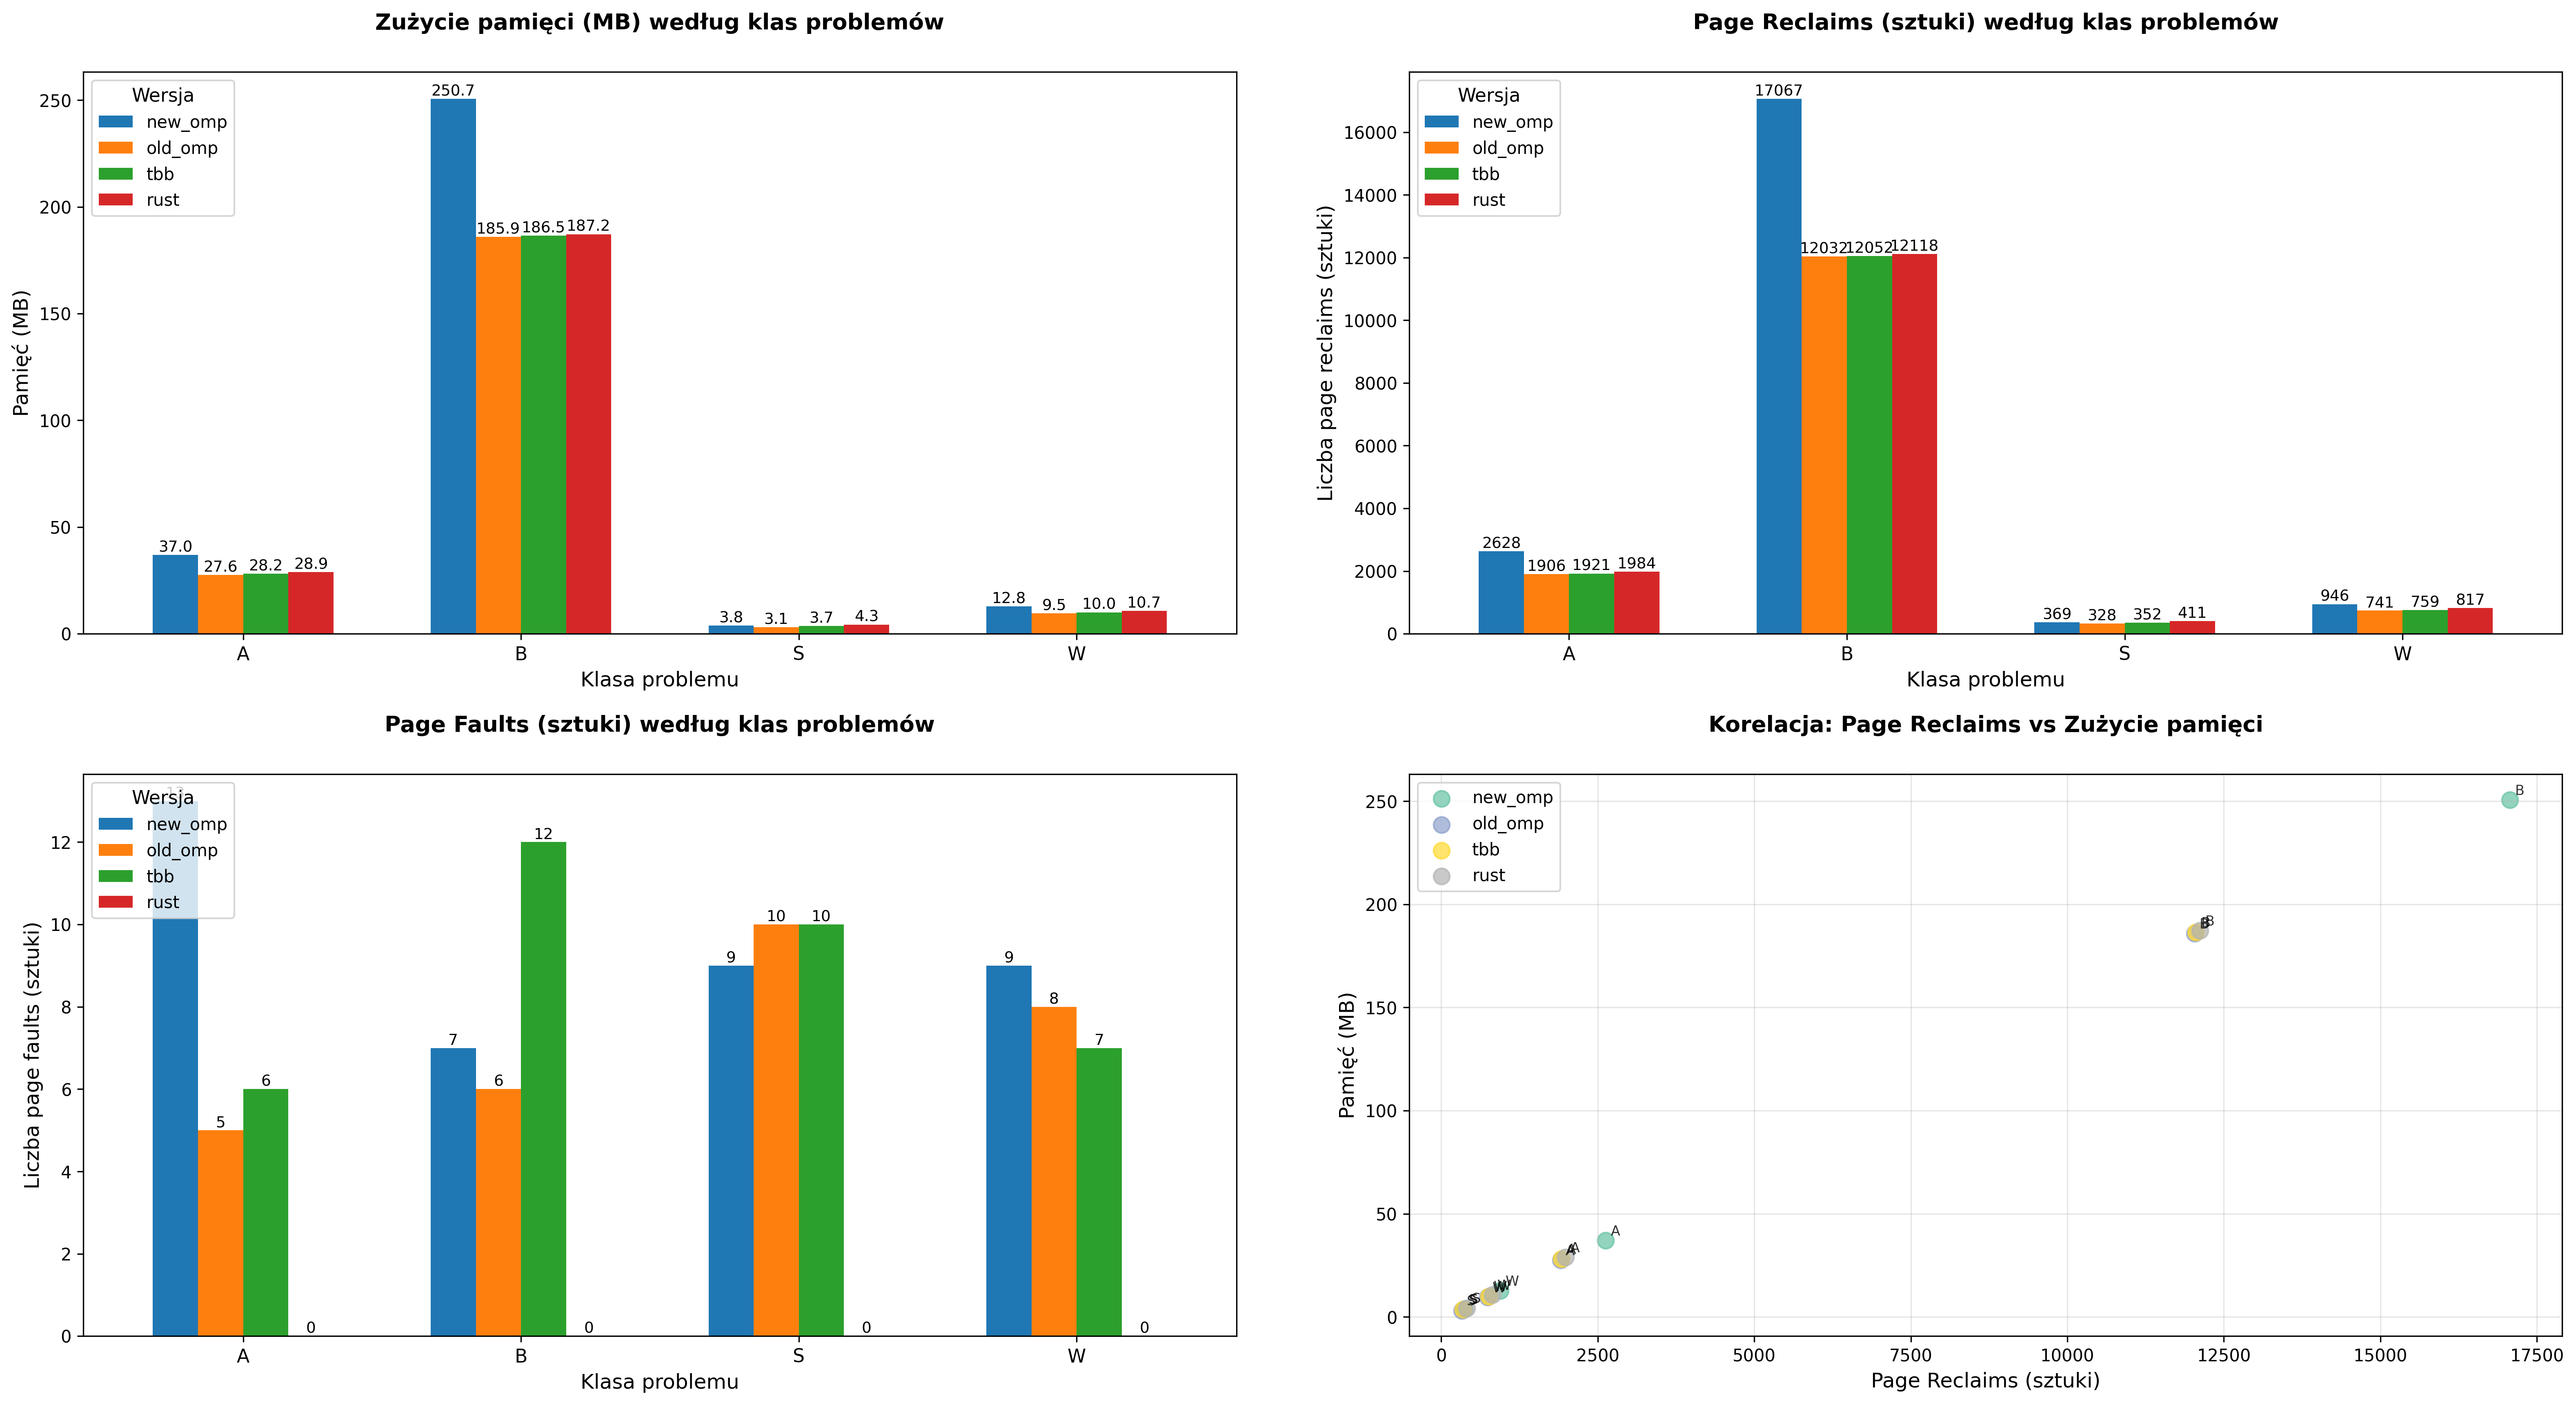
\includegraphics[width=\textwidth]{analiza/images/parallel/cg/arm/chart_01_memory_comparison.png}
    \caption{Profilowanie wydajności benchmarku CG dla klas S, W, A, B względem liczby użytych wątków na platformie ARM64}
    \label{cg_porownanie_zuzycia_pamieci}
\end{figure}

\subsubsection{Zużycie pamięci (MB)}
Na pierwszym wykresie - rysunek \ref{cg_porownanie_zuzycia_pamieci} (lewy górny róg) przedstawiono zużycie pamięci operacyjnej (w MB) dla czterech wersji implementacji algorytmu:
\begin{itemize}
    \item W klasie problemu B występuje najwyższe zużycie pamięci we wszystkich wersjach. Szczególnie zauważalny jest wynik dla new\_omp (250,7 MB), który znacząco przekracza wartości dla pozostałych wersji (około 185-187 MB).
    \item W klasie A new\_omp również zużywa najwięcej pamięci (37 MB), natomiast pozostałe wersje wykazują zbliżony i niższy poziom zużycia (około 27-29 MB).
    \item W klasach S i W różnice są mniej wyraźne, jednak nadal new\_omp wykazuje największe zużycie pamięci.
    \item Wersja rust generalnie charakteryzuje się najmniejszym lub jednym z najmniejszych zużyć pamięci w większości klas problemów.
\end{itemize}

\subsubsection{Liczba zwalniania stron pamięci (sztuki)}
Drugi wykres - rysunek \ref{cg_porownanie_zuzycia_pamieci} (prawy górny róg) ilustruje liczbęzwalniania stron pamięci \eng{page reclaim}, czyli sytuacji, w których system operacyjny odzyskuje strony pamięci.
\begin{itemize}
    \item Najwięcej zwalnianych stron pamięci występuje w klasie B dla wersji new\_omp (17067), co koresponduje z jej wysokim zużyciem pamięci.
    \item W pozostałych wersjach liczba zwolnionych stron w klasie B jest znacznie niższa (około 12000-12100).
    \item W klasie A new\_omp ponownie osiąga najwyższy wynik (2628), przy niższych wartościach pozostałych wersji (około 1900).
    \item W klasach S i W różnice są mniej zauważalne, choć new\_omp nadal wykazuje wyższe wartości.
\end{itemize}

\subsubsection{Odwołania do nieobecnych stron (sztuki)}

Trzeci wykres - rysunek \ref{cg_porownanie_zuzycia_pamieci} (lewy dolny róg) przedstawia odwołania do nieobecnych stronliczbę \eng{page fault} - czyli sytuacji, w których wymagany fragment pamięci nie znajduje się aktualnie w RAM-ie.
\begin{itemize}
    \item W klasie A new\_omp wykazuje najwyższą liczbę page faults (13), zaś rust nie generuje żadnych błędów.
    \item W klasie B najwięcej błędów generuje TBB (12), podczas gdy rust ponownie nie wykazuje żadnych.
    \item W klasach S i W rust również nie generuje page faults, a inne wersje wykazują umiarkowane wartości (7-10).
    \item Wyniki te sugerują bardzo efektywną gospodarkę pamięciową w wersji rust.
\end{itemize}

\subsubsection{Korelacja: Liczba zwalniania stron pamięci vs Zużycie pamięci}
Ostatni wykres - rysunek \ref{cg_porownanie_zuzycia_pamieci} (prawy dolny róg) ilustruje zależność pomiędzy liczbą zwolnionych stron pamięci a zużyciem pamięci.
\begin{itemize}
    \item Widoczna jest silna dodatnia korelacja - im większe zużycie pamięci, tym większa liczba zwolnionych stron pamięci. Najwyraźniejszym punktem odniesienia jest wersja new\_omp dla klasy B, która dominuje pod względem obu metryk.
    \item Punkty reprezentujące wersję rust znajdują się w lewej dolnej części wykresu, wskazując na niskie zużycie pamięci i małą liczbę zwolnionych stron.
\end{itemize}

\begin{figure}[H]
    \centering
    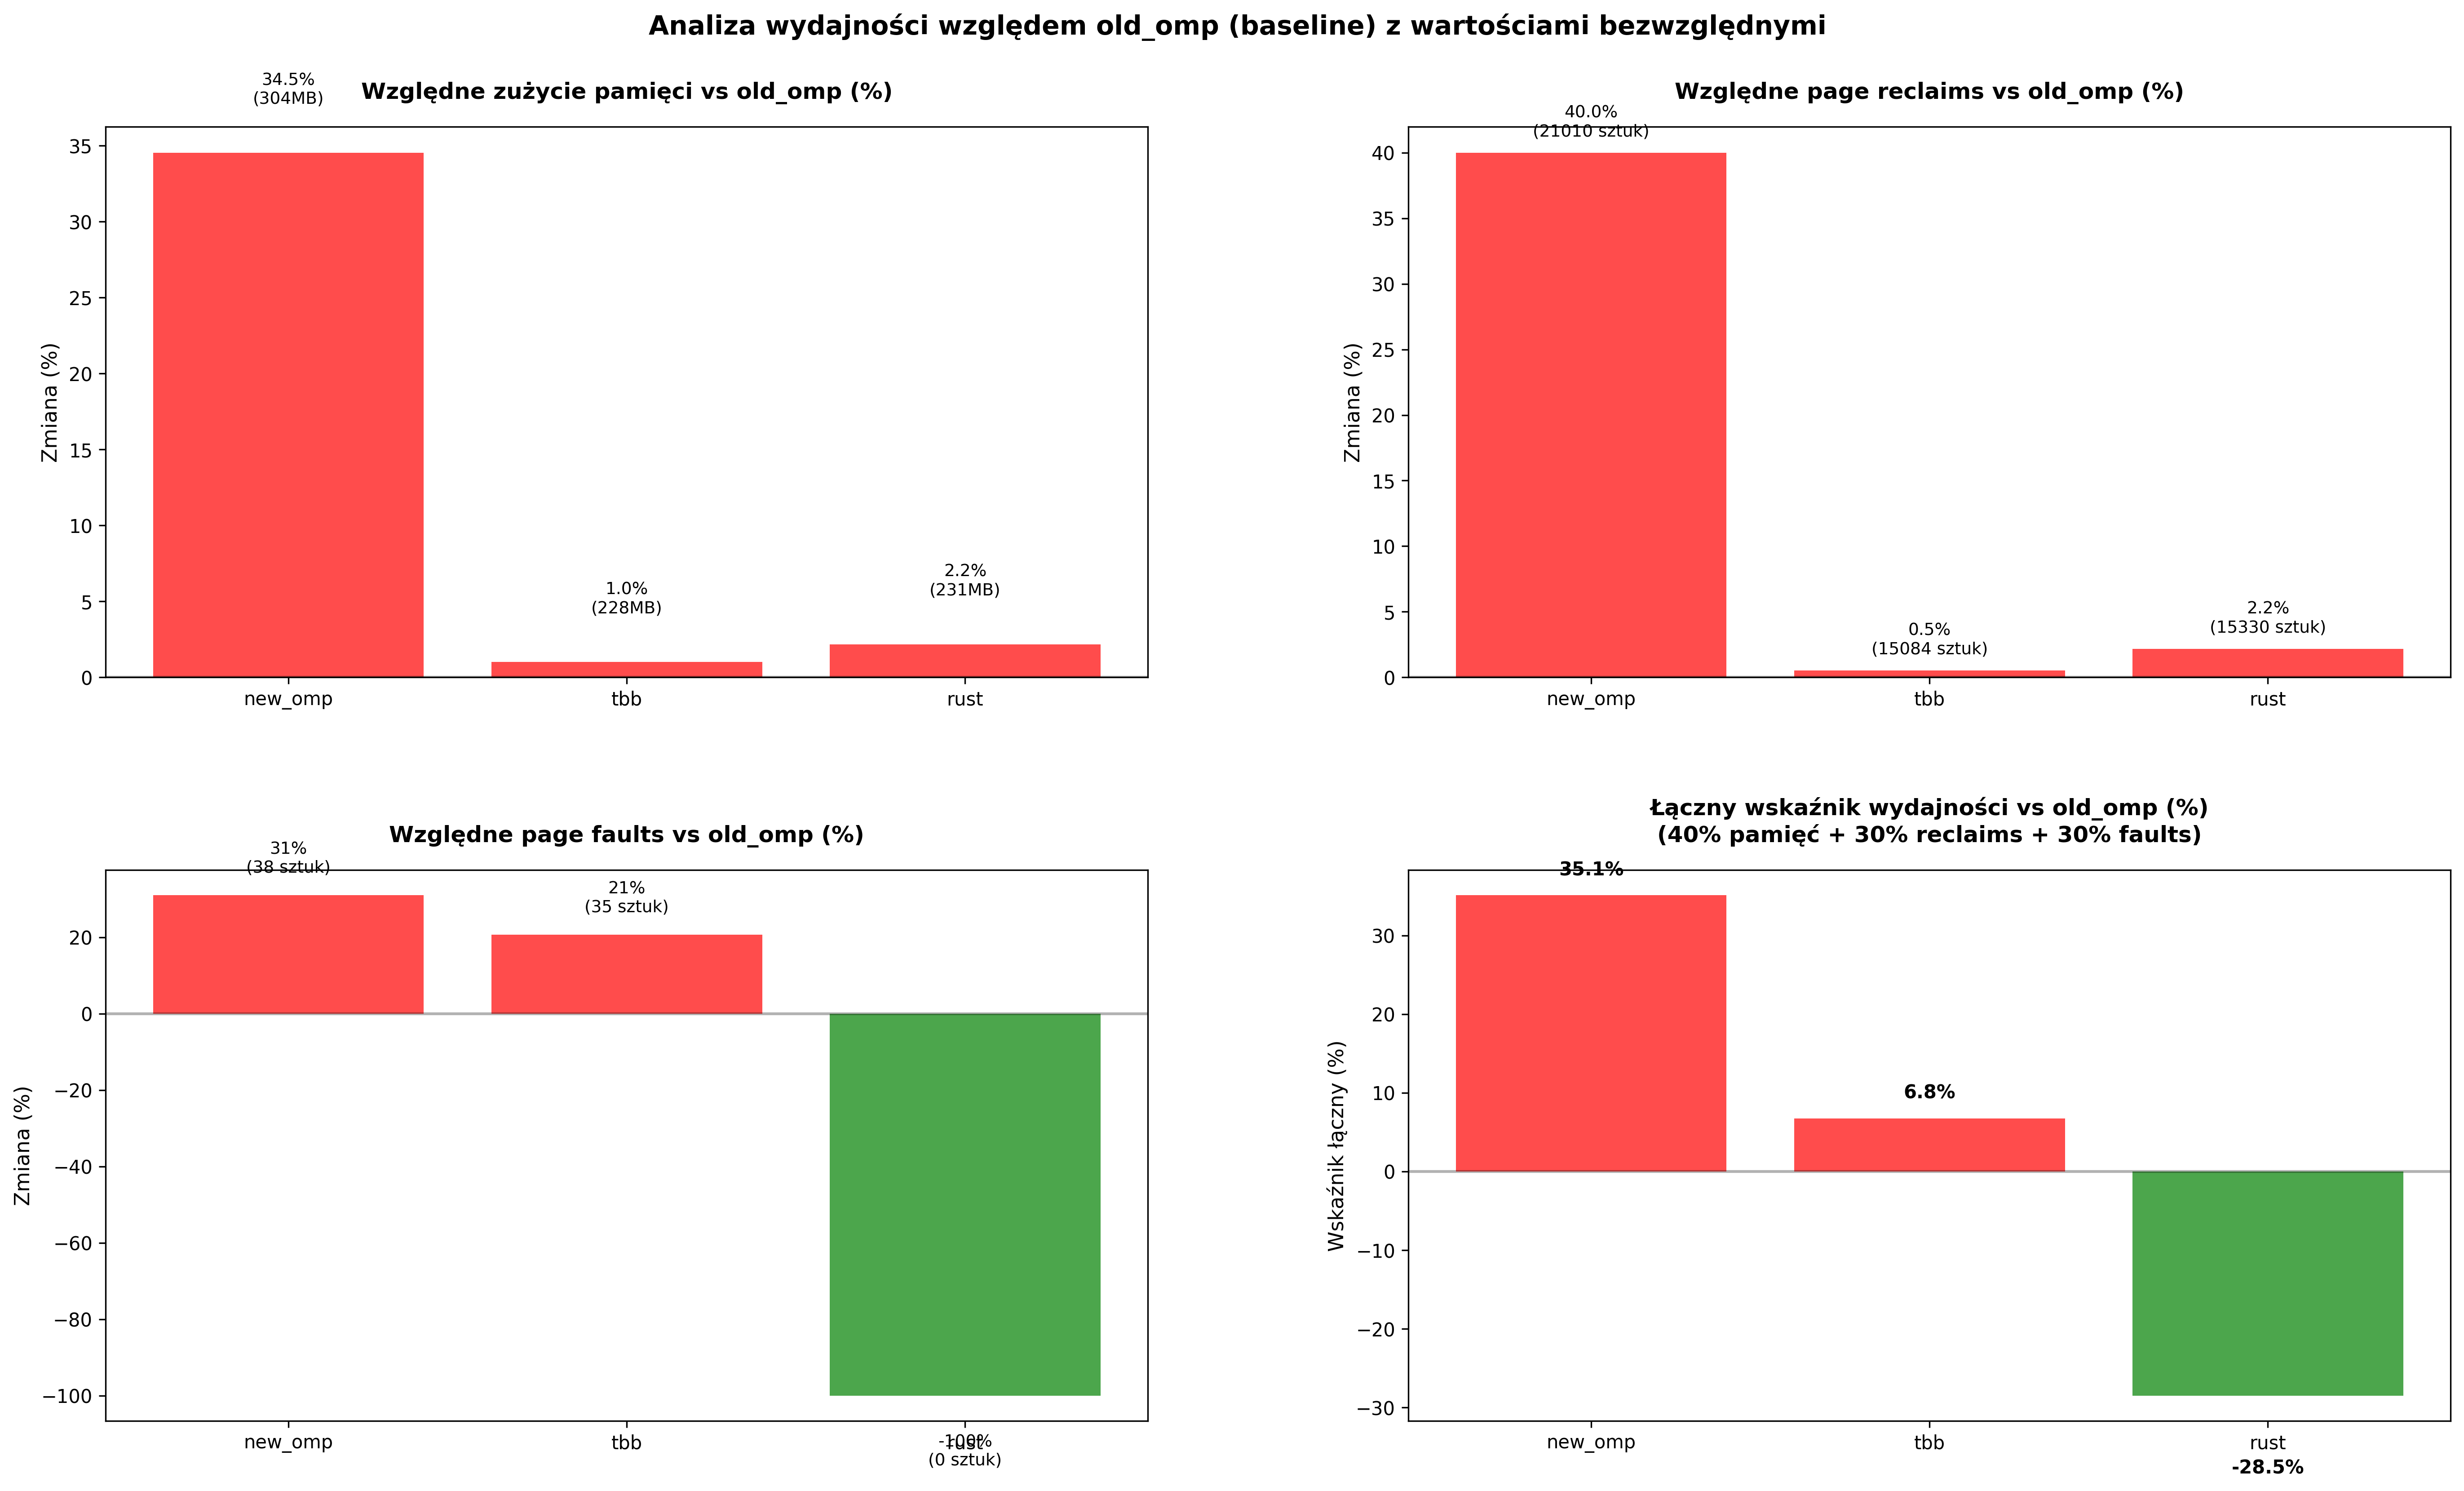
\includegraphics[width=\textwidth]{analiza/images/parallel/cg/arm/chart_05_performance_ratios.png}
    \caption{Analiza wydajności względem old\_omp (punkt odniesienia) z wartościami bezwzględnymi na platformie ARM64}
    \label{cg_analiza_wzgledem_old_omp}
\end{figure}
Na wykresie - rysunek \ref{cg_analiza_wzgledem_old_omp} szczegółowa analiza czterech wykresów przedstawiających względną wydajność trzech wersji implementacji (new\_omp, TBB, rust) względem wersji bazowej old\_omp. Analiza dotyczy zużycia pamięci, liczby zwolnionych stron pamięci, odwołań do nieobecncyh stron oraz skumulowanego wskaźnika efektywności.
\subsubsection{Względne zużycie pamięci vs old\_omp}
Pierwszy wykres - rysunek \ref{cg_analiza_wzgledem_old_omp} (lewy górny róg) ukazuje procentową zmianę w zużyciu pamięci operacyjnej względem implementacji referencyjnej. Największy wzrost odnotowano dla new\_omp, gdzie zużycie pamięci wzrosło o 34,5\%, co przekłada się na dodatkowe 304 MB. Zmiany dla TBB i rust były marginalne i wyniosły odpowiednio 1,0\% (228 MB) oraz 2,2\% (231 MB), co sugeruje ich większą efektywność w kontekście gospodarowania pamięcią.

\subsubsection{Względne odzyskiwanie stron pamięci vs old\_omp}
Drugi wykres - rysunek \ref{cg_analiza_wzgledem_old_omp} (prawy górny róg) przedstawia zmiany w liczbie odzyskanych stron pamięci. Implementacja new\_omp wykazała aż 40\% wzrost (21010 stron), co może świadczyć o intensywnym zarządzaniu pamięcią w trakcie wykonywania programu. Dla TBB i rust zmiany były minimalne (odpowiednio 0,5\% i 2,2\%), co może być interpretowane jako korzystny efekt optymalizacji dostępu do pamięci.

\subsubsection{Względne błędy stron vs old\_omp}
Na trzecim wykresie - rysunek \ref{cg_analiza_wzgledem_old_omp} (lewy dolny róg) obserwujemy względną liczbę błędów stron. new\_omp i TBB odnotowały wzrost liczby błędów stron odpowiednio o 31\% (38 sztuk) i 2\% (35 sztuk), co może wskazywać na mniej wydajne wykorzystanie pamięci w porównaniu z old\_omp. Z kolei rust jako jedyna implementacja odnotowała całkowitą eliminację błędów stron (-100\%, 0 sztuk), co potwierdza wyjątkowo skuteczną kontrolę pamięci operacyjnej - mechanizmy własności oraz pożyczania.

\subsubsection{Łączny wskaźnik wydajności vs old\_omp}
Na ostatnim wykresie - rysunek \ref{cg_analiza_wzgledem_old_omp} (prawy dolny róg) przedstawiono zagregowany wskaźnik wydajności, będący ważoną sumą trzech poprzednich metryk: 40\% udziału zużycia pamięci, 30\% udziału odzyskiwania stron oraz 30\% udziału błędów stron. Najwyższy wskaźnik (35,1\%) ponownie osiąga new\_omp, co oznacza wyraźnie wyższą konsumpcję zasobów w porównaniu do referencji. TBB wykazuje niewielki wzrost (6,8\%), co czyni go względnie neutralnym względem old\_omp. rust natomiast charakteryzuje się łącznym wskaźnikiem na poziomie -28,5\%, co czyni go najbardziej efektywną implementacją w ujęciu ogólnym.

\begin{figure}[H]
    \centering
    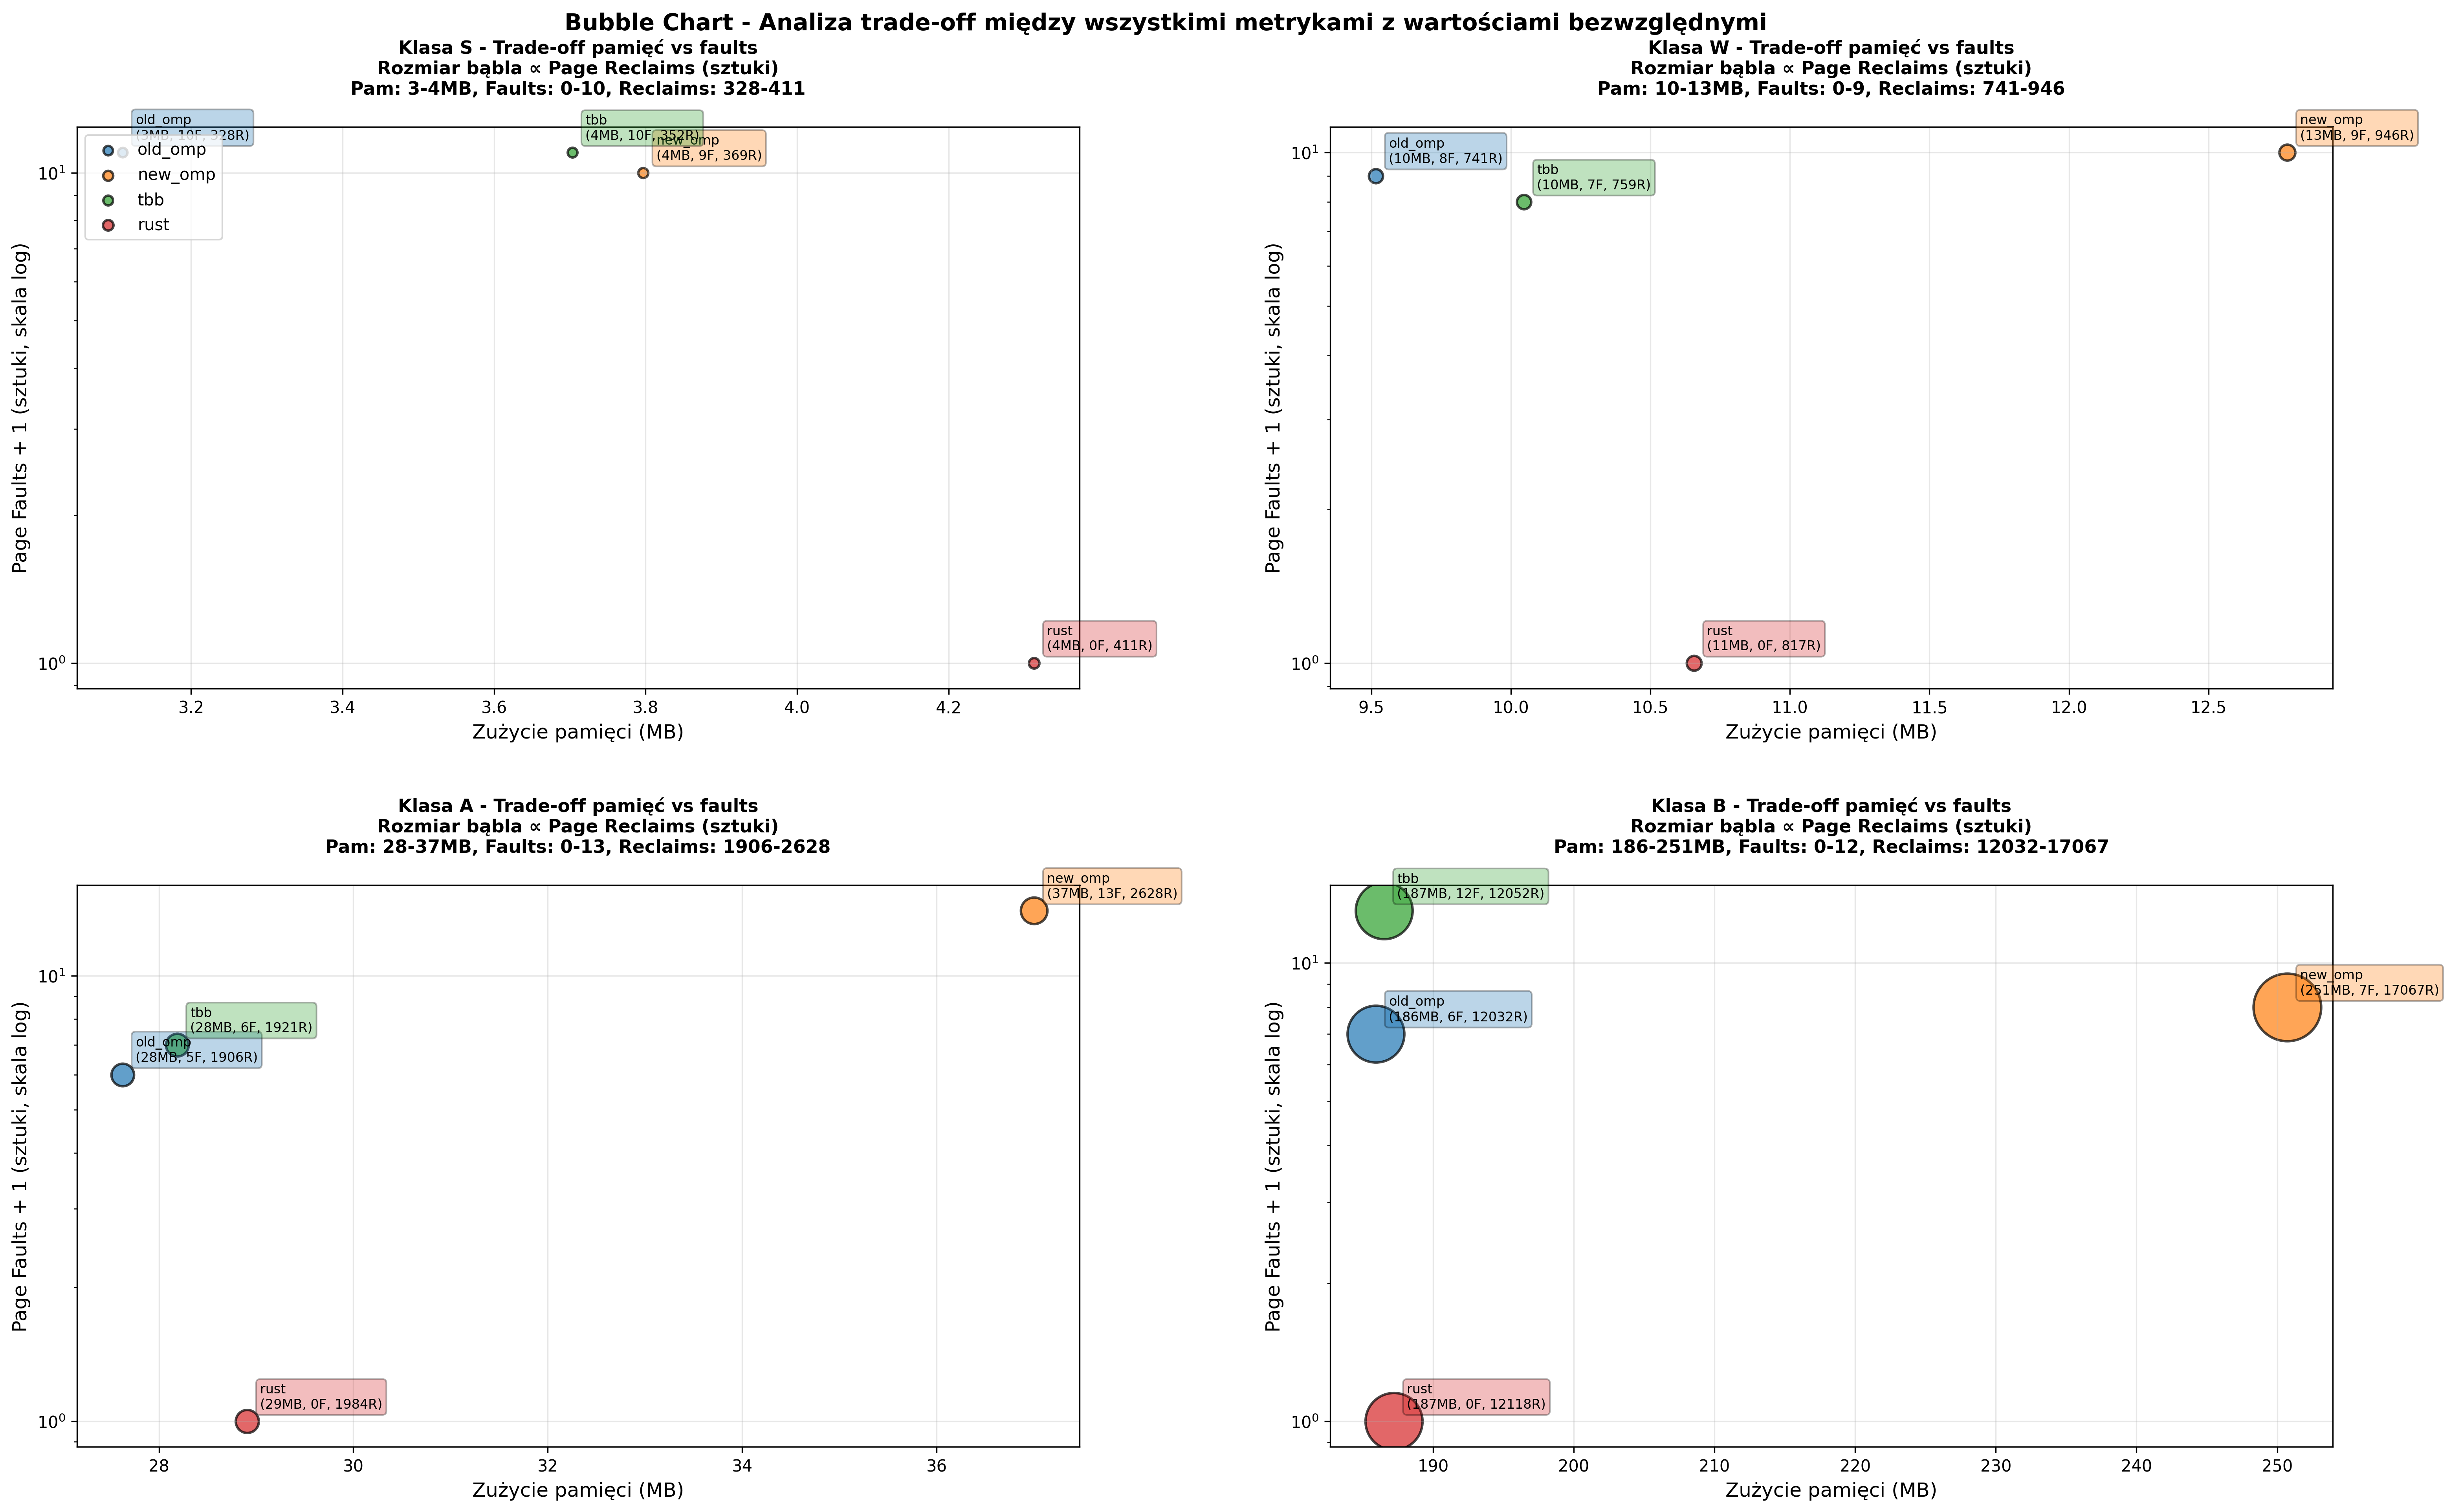
\includegraphics[width=\textwidth]{analiza/images/parallel/cg/arm/chart_06_bubble_chart.png}
    \caption{Kompromisy \eng{trade-off} pomiędzy zużyciem pamięci a błędami stron pamięci, z uwzględnieniem liczby odzyskanych stron jako trzeciej zmiennej reprezentowanej przez rozmiar bąbla na platformie ARM64}
    \label{cg_kompromisy_pamiec_bledy}
\end{figure}

W celu całościowej oceny efektywności pamięciowej badanych implementacji, opracowano wykresy - rysunek \ref{cg_kompromisy_pamiec_bledy} typu "bubble chart”, które ukazują kompromisy między dwiema kluczowymi metrykami: zużyciem pamięci oraz liczbą błędów stron. Wykresy te wzbogacono o trzeci wymiar - liczbę odzyskanych stron pamięci, która została zakodowana poprzez rozmiar bąbla. Wszystkie wartości przedstawiono w postaci bezwzględnej, przy czym oś Y jest skalowana logarytmicznie w celu lepszego rozróżnienia niewielkich wartości.

Każdy z czterech wykresów odpowiada innej klasie obciążenia pamięciowego (S, W, A, B), przy czym wspólnym celem ich analizy jest uchwycenie relacji pomiędzy wzrostem zużycia pamięci a pogorszeniem lub poprawą stabilności działania (mierzonej błędami stron) oraz intensywnością operacji odzyskiwania stron.

W skali globalnej można zaobserwować, że implementacja rust wielokrotnie wypada korzystnie - cechuje się niskim zużyciem pamięci, zerową liczbą błędów stron w wielu przypadkach oraz stosunkowo niską liczbą zwolnień, co sugeruje wysoką efektywność i dobrą kontrolę nad zarządzaniem pamięcią. Z kolei new\_omp, mimo czasem lepszych wyników obliczeniowych, wykazuje największe zużycie pamięci oraz relatywnie wysoką liczbę błędów stron i odzysków pamięci, co może oznaczać znaczną presję na system zarządzania pamięcią operacyjną.

Implementacja TBB prezentuje wyniki pośrednie, w niektórych przypadkach zbliżone do old\_omp, ale przy lepszym wykorzystaniu zasobów - co czyni ją kompromisowym rozwiązaniem o umiarkowanej efektywności.
-
\subsection{Wyniki profilowania wydajności - platforma x86\_64}
\begin{figure}[H]
    \centering
    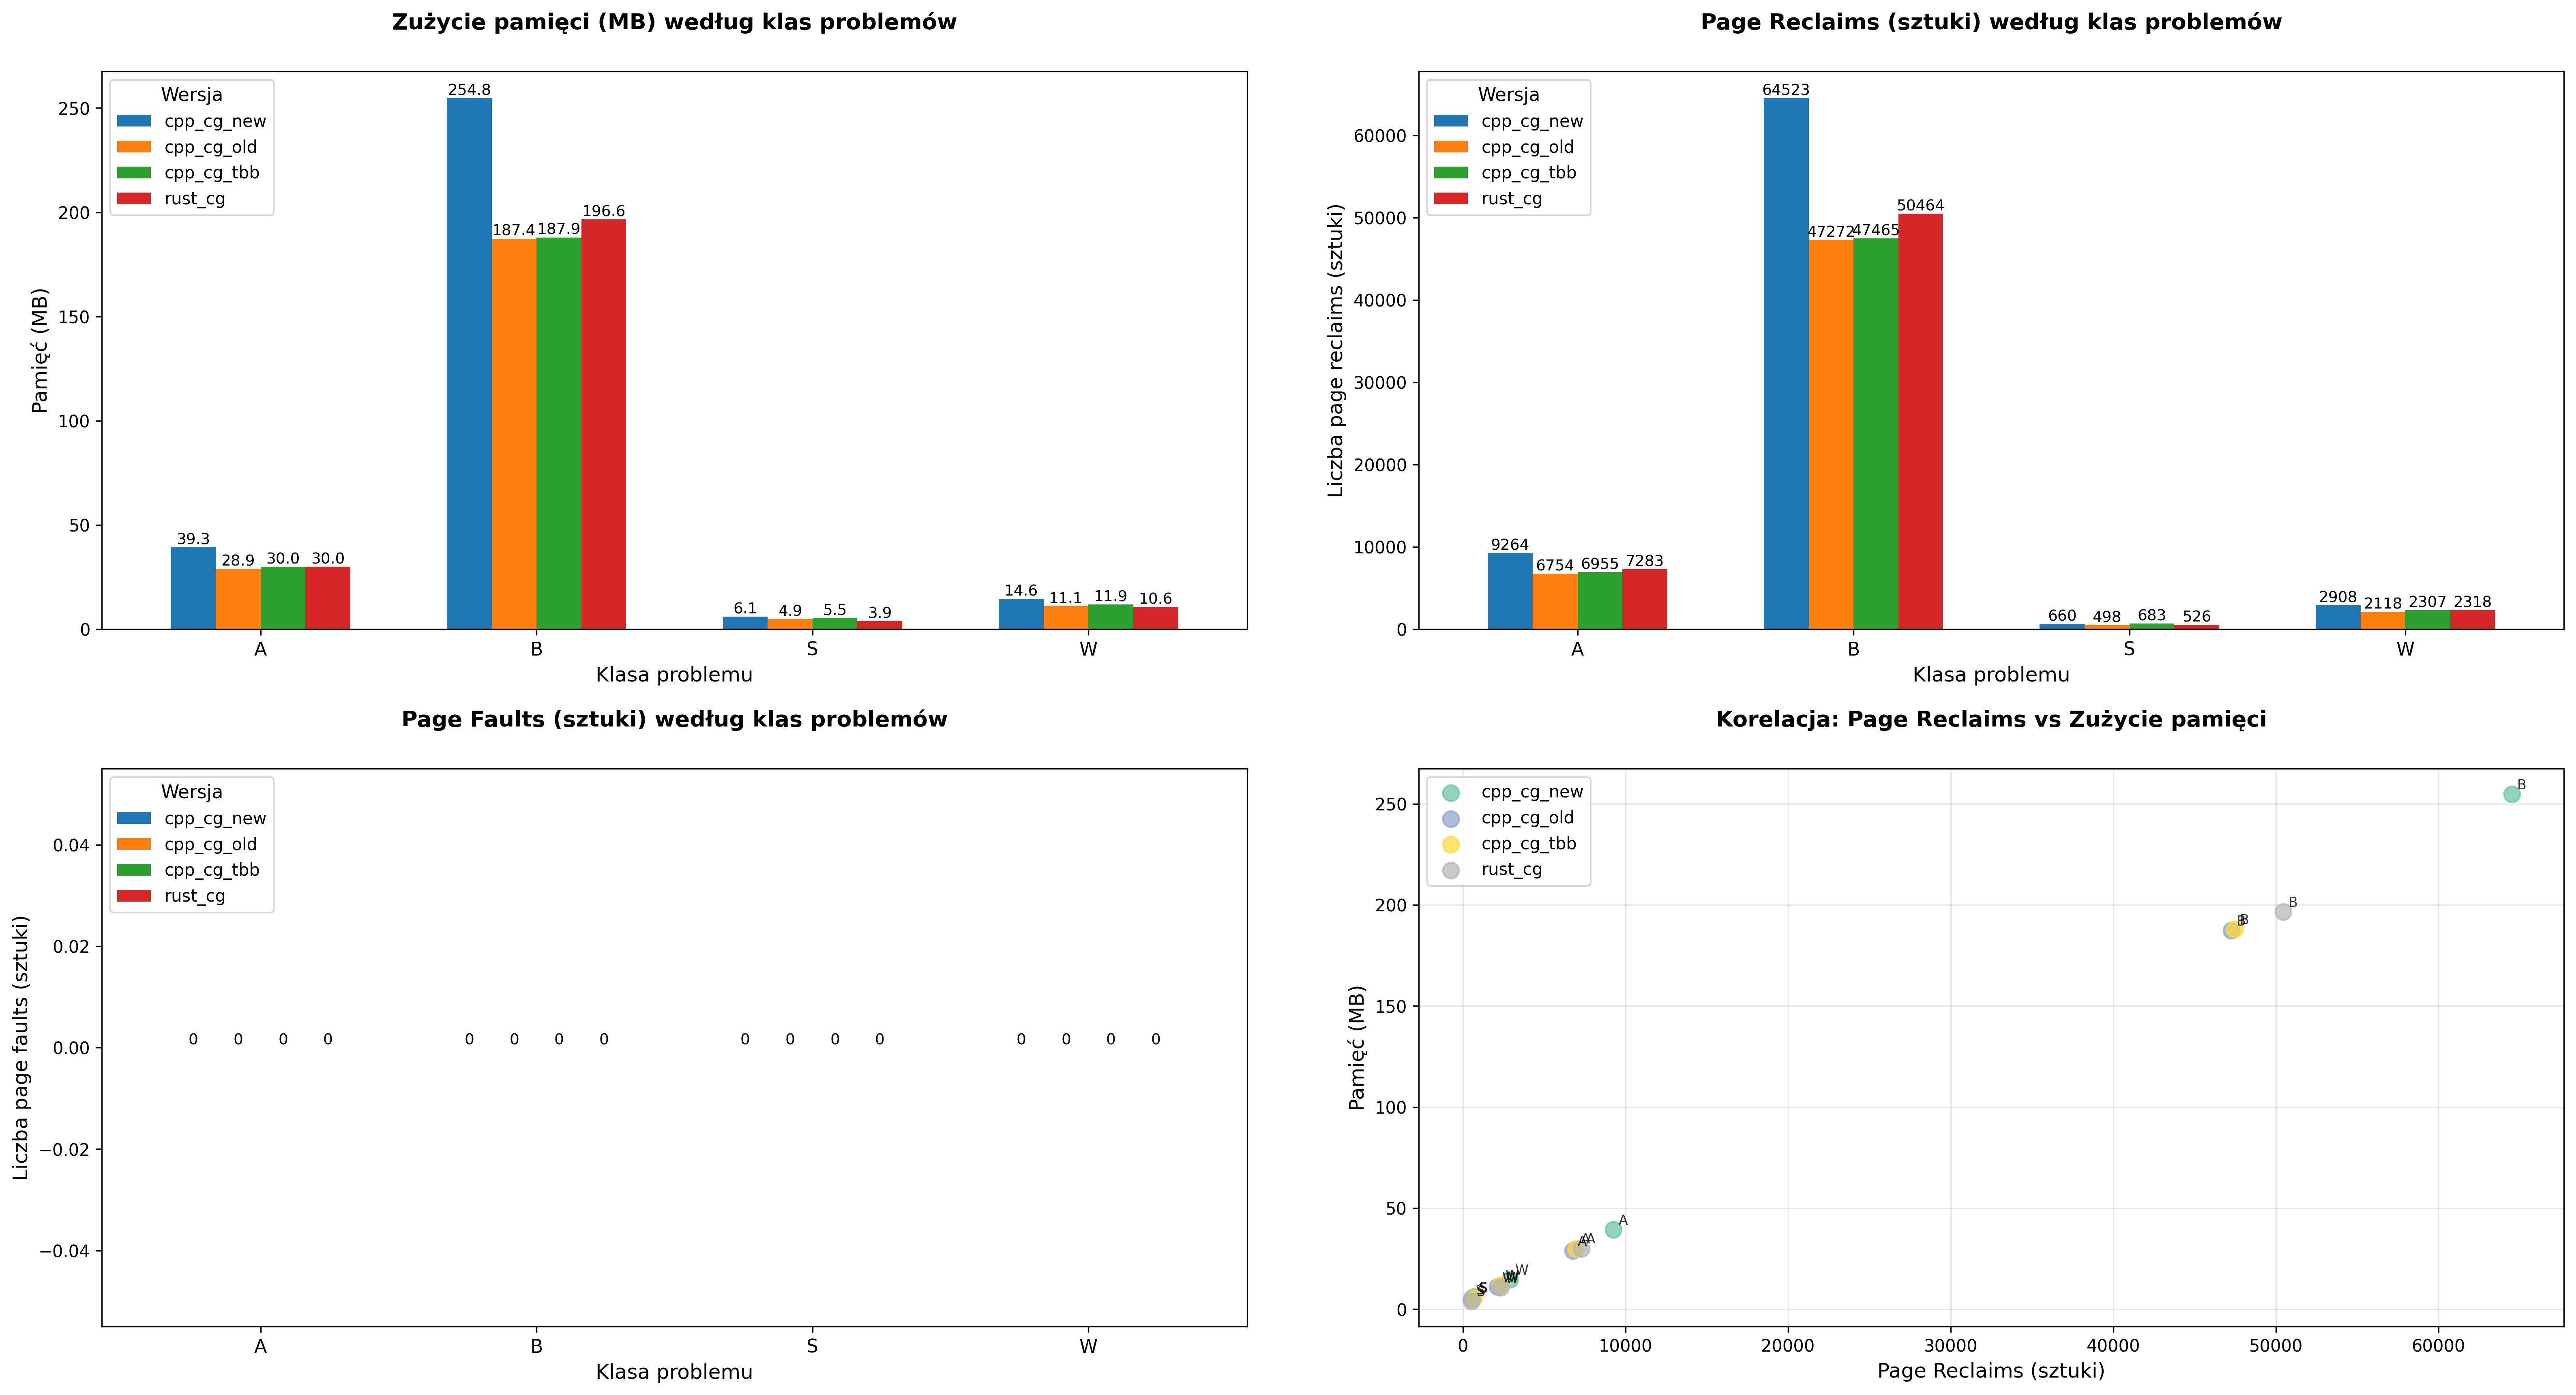
\includegraphics[width=\textwidth]{analiza/images/parallel/cg/x86/chart_01_memory_comparison.png}
    \caption{Profilowanie wydajności benchmarku CG dla klas S, W, A, B względem liczby użytych wątków na platformie x86\_64}
    \label{cg_porownanie_zuzycia_pamieci_x86_64}
\end{figure}
\subsubsection{Zużycie pamięci (MB)}
Z wykresu - rysunek \ref{cg_porownanie_czasow_wykonania_x86_64} zużycia pamięci wynika, że implementacja new\_omp jest zdecydowanie najbardziej pamięciożerna w klasie B, gdzie osiąga wartość 254,8 MB — to istotnie więcej niż pozostałe implementacje, które utrzymują się w zakresie 187-197 MB. Dla pozostałych klas (A, S, W) różnice pomiędzy implementacjami są znikome i mieszczą się w przedziale od 3,9 MB do 39,3 MB.

Zależność zużycia pamięci od klasy problemu jest zgodna z oczekiwaniami: większa klasa (większy problem obliczeniowy) wiąże się z wyższym zużyciem zasobów. Jednak istotna różnica dla new\_omp w klasie B sugeruje potencjalne niedoskonałości w zarządzaniu pamięcią lub większy narzut alokacyjny tej wersji.

\subsubsection{Operacje Page Reclaim (sztuki)}
Podobnie jak w przypadku zużycia pamięci, new\_omp generuje najwyższe liczby operacji zwolnień stron — w klasie B sięgają one ponad 64 tys. Operacje te wskazują na intensywną aktywność zarządzania pamięcią przez system operacyjny i mogą prowadzić do pogorszenia wydajności w warunkach ograniczonych zasobów. Pozostałe implementacje generują wyraźnie mniej takich operacji (ok. 47-50 tys. dla klasy B).

W klasach A, S i W różnice między implementacjami są mniej znaczące. Warto jednak zwrócić uwagę, że rust we wszystkich klasach cechuje się stosunkowo niskim poziomem zwolnień, co może świadczyć o bardziej efektywnym wykorzystaniu pamięci przez alokator w środowisku Rust.

\subsubsection{Page Faults (sztuki)}
Wszystkie implementacje, niezależnie od klasy problemu, wykazują zerowy poziom błędów stron. Taki wynik jest pozytywny i świadczy o prawidłowej alokacji oraz dostępie do pamięci bez potrzeby kosztownego przenoszenia stron pamięci z dysku do RAM-u. To również sugeruje, że żadne z testów nie spowodowały przeciążenia systemu w zakresie dostępnej pamięci fizycznej.

\subsubsection{Korelacja: Liczba zwalniania stron pamięci vs Zużycie pamięci}
Wykres rozrzutu przedstawia silną dodatnią korelację pomiędzy liczbą operacji zwolnień stron a zużyciem pamięci. Punkty odpowiadające klasie B znajdują się wyraźnie w prawym górnym rogu wykresu, potwierdzając, że najbardziej zasobożerna klasa problemu generuje również najwięcej interakcji z systemowym menedżerem pamięci. Punkty dla klas A, S i W rozmieszczone są blisko siebie w lewym dolnym obszarze, co wskazuje na relatywnie stabilne i niskie zużycie pamięci.

\subsubsection{Nota wyjaśniająca}
Ze względu na brak błędów stron nie zamieszczono pozostałych wykresów, które byłyby oparte na tej metryce. Wykresy te nie miałyby sensu, ponieważ brak błędów stron oznacza, że wszystkie operacje pamięciowe były realizowane w ramach dostępnej pamięci fizycznej bez konieczności angażowania mechanizmów swapowania lub przenoszenia stron z dysku.

\subsection{Porównanie pomiędzy platformami}
\subsubsection{Średnia wydajność i współczynnik przyspieszenia}
\begin{figure}[H]
    \centering
    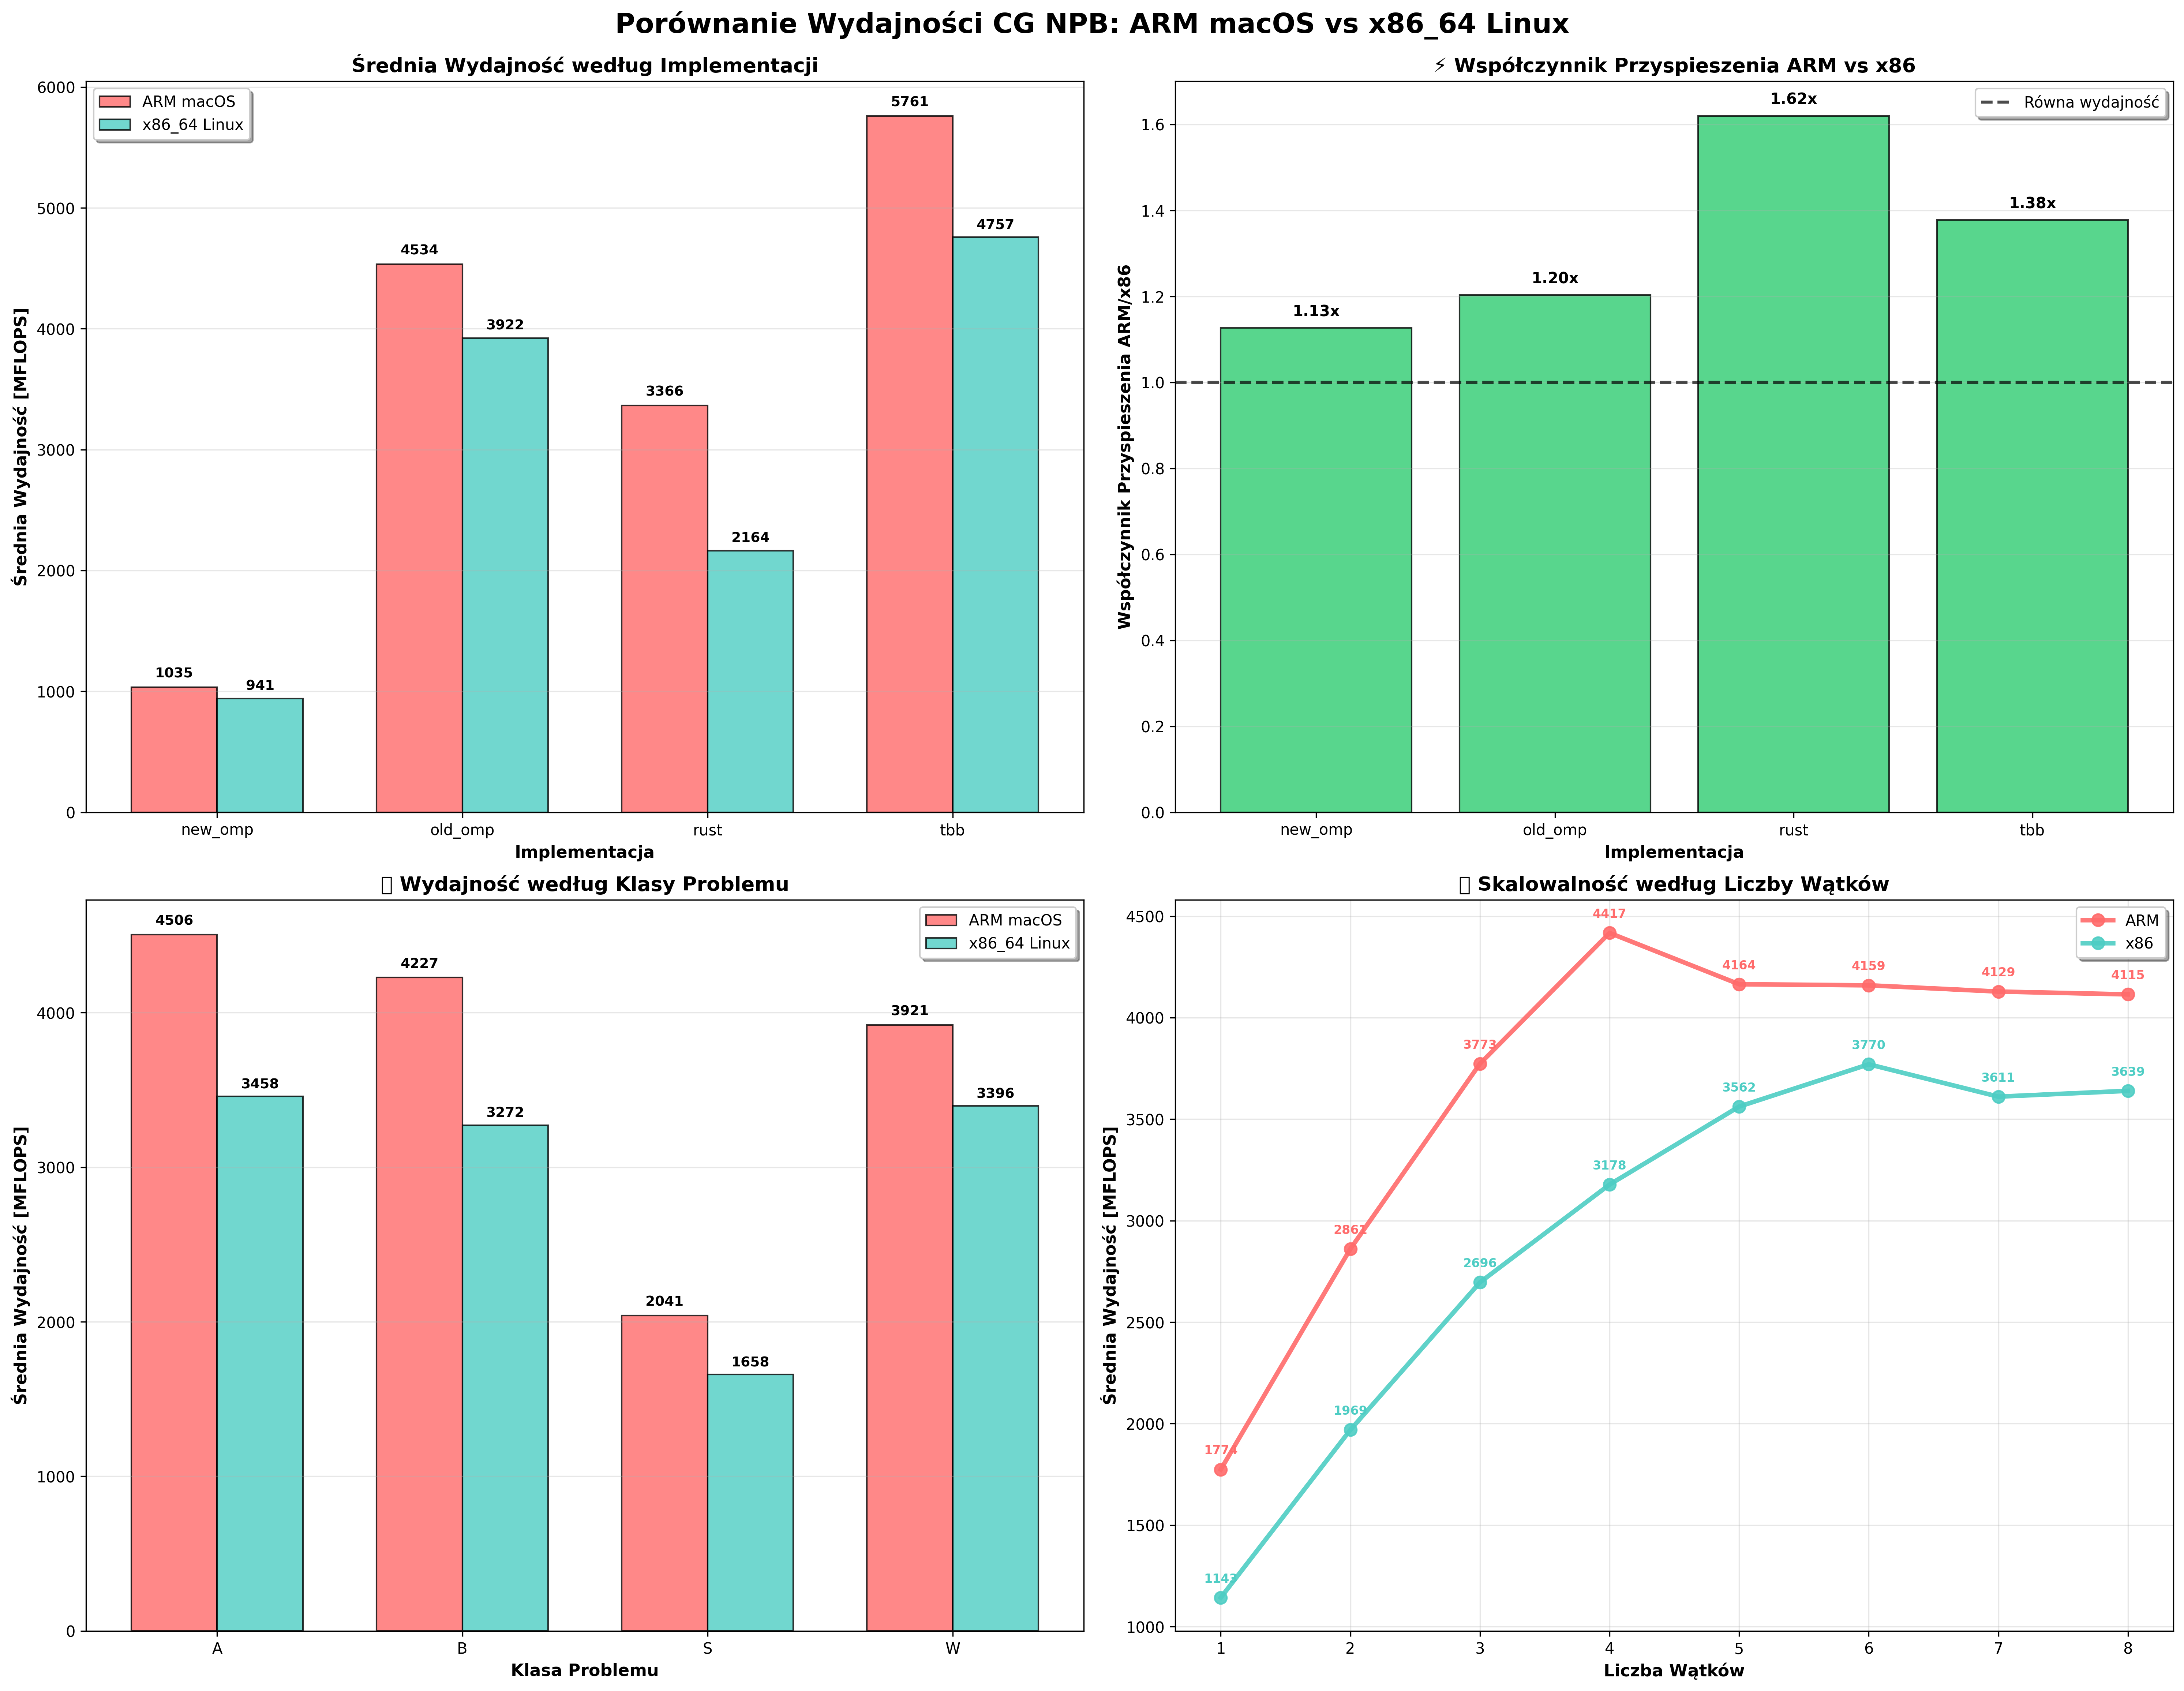
\includegraphics[width=\textwidth]{analiza/images/parallel/cg/compare/cg_porownanie_platform_arm_vs_x86.png}
    \caption{Porównanie średniej wydajności benchmarku CG dla platform ARM64 i x86\_64}
    \label{cg_porownanie_platform_arm_vs_x86}
\end{figure}
Na podstawie wykresów - rysunek \ref{cg_porownanie_platform_arm_vs_x86} uśrednionej wydajności (wyrażonej w MFLOPS) można zaobserwować, że implementacje benchmarku CG uzyskują zróżnicowane rezultaty na obu platformach. Najwyższą wydajność osiąga implementacja tbb na obu architekturach, przy czym wynik dla ARM (5761 MFLOPS) jest wyższy niż dla x86 (4757 MFLOPS). Implementacja rust również wypada lepiej na platformie ARM, uzyskując przewagę nad x86 rzędu 62\% (współczynnik przyspieszenia ARM/x86 = 1.62).

Z kolei old\_omp i new\_omp wykazują mniejsze różnice pomiędzy platformami, jednak nadal na korzyść ARM (współczynnik przyspieszenia odpowiednio 1.20 i 1.13). Pokazuje to, że układy ARM, mimo mniejszej popularności w obliczeniach naukowych, mogą zapewniać porównywalną lub wyższą wydajność w zadaniach równoległych.
\subsubsection{Wydajność względem klasy problemu}
Dla wszystkich klas problemu platforma ARM uzyskuje wyższe wartości MFLOPS w porównaniu do x86, przy czym różnice te są szczególnie widoczne w klasach A i B — odpowiednio 4506 vs 3458 oraz 4227 vs 3272 MFLOPS. Mniejsze różnice występują w klasach S i W, co może być związane z ograniczoną skalowalnością w mniejszych problemach oraz różnicami w architekturze pamięci podręcznej.
\subsubsection{Skalowanie według liczby wątków}
Analiza wykresu skalowalności pokazuje, że ARM osiąga wyższe wartości MFLOPS w niemal każdej konfiguracji wątkowej. Dla 4 wątków uzyskuje wartość 4417 MFLOPS, przewyższając tym samym x86 (3179 MFLOPS). Mimo że przy wzroście liczby wątków następuje spłaszczenie wykresów dla obu platform, ARM utrzymuje przewagę aż do 8 wątków, co potwierdza dobre skalowanie procesora ARM w tej klasie obliczeń.

\begin{figure}[H]
    \centering
    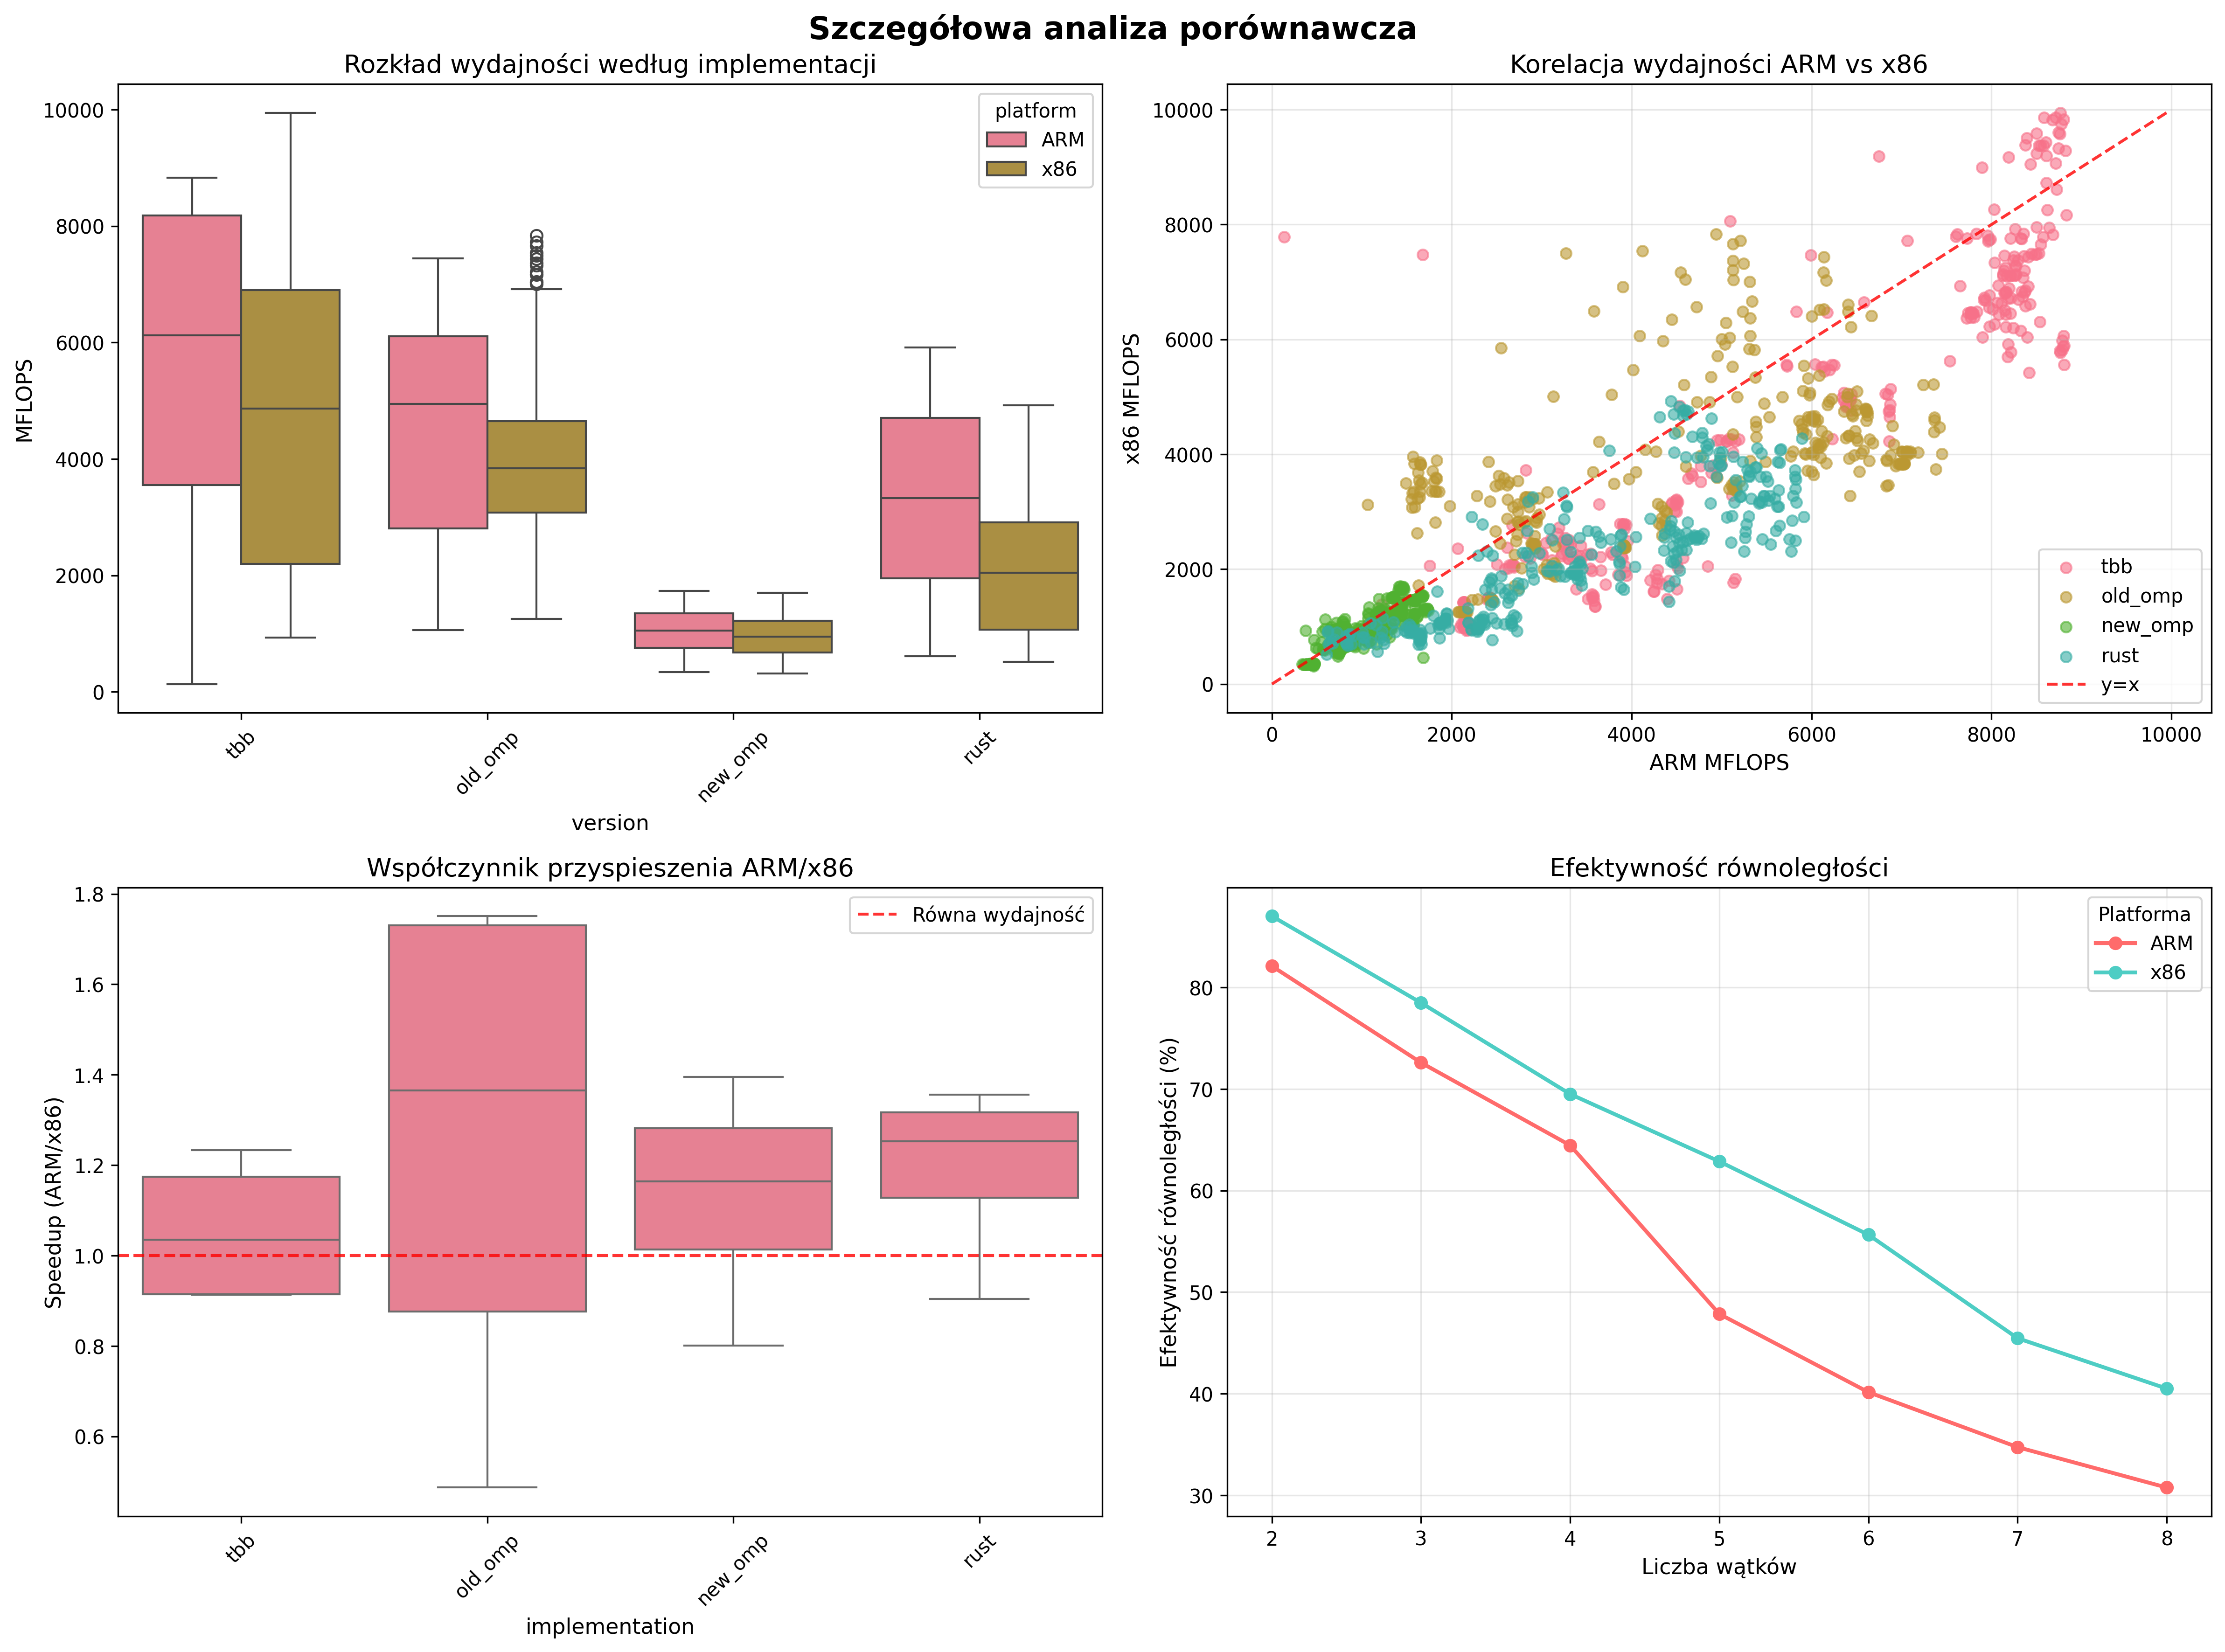
\includegraphics[width=\textwidth]{analiza/images/parallel/cg/compare/cg_szczegolowa_analiza_wydajnosci.png}
    \caption{Szczegółowa analiza wydajności benchmarku CG dla platform ARM64 i x86\_64}
    \label{cg_szczegolowa_analiza_wydajnosci}
\end{figure}
\subsubsection{Rozkład wydajności i korelacja}
Wykres pudełkowy obrazujące rozkład wydajności według implementacji pokazują większą zmienność wyników na platformie ARM, szczególnie dla tbb i old\_omp, co może świadczyć o bardziej dynamicznym zarządzaniu zasobami na poziomie systemowym (macOS). Mimo tej zmienności, wartości median są konsekwentnie wyższe dla ARM.

Wykres korelacyjny MFLOPS ARM vs x86 ukazuje silną dodatnią korelację między wynikami na obu platformach, z większością punktów powyżej linii równej wydajności (y = x), co oznacza, że ARM zazwyczaj przewyższa x86 pod względem osiągów. W przypadku rust różnica jest szczególnie wyraźna.

\subsubsection{Efektywność równoległości}
Analiza efektywności równoległości (rozumianej jako stosunek osiągniętej wydajności do liczby wątków względem wydajności jednordzeniowej) wskazuje na wyraźnie wyższe wartości dla platformy x86 przy większej liczbie wątków. Podczas gdy ARM charakteryzuje się dobrą wydajnością bezwzględną, jego efektywność maleje szybciej wraz ze wzrostem liczby wątków, co może wynikać z wąskiego gardła na poziomie pamięci współdzielonej lub mniejszej liczby jednostek wykonawczych na wątek fizyczny.

\begin{figure}[H]
    \centering
    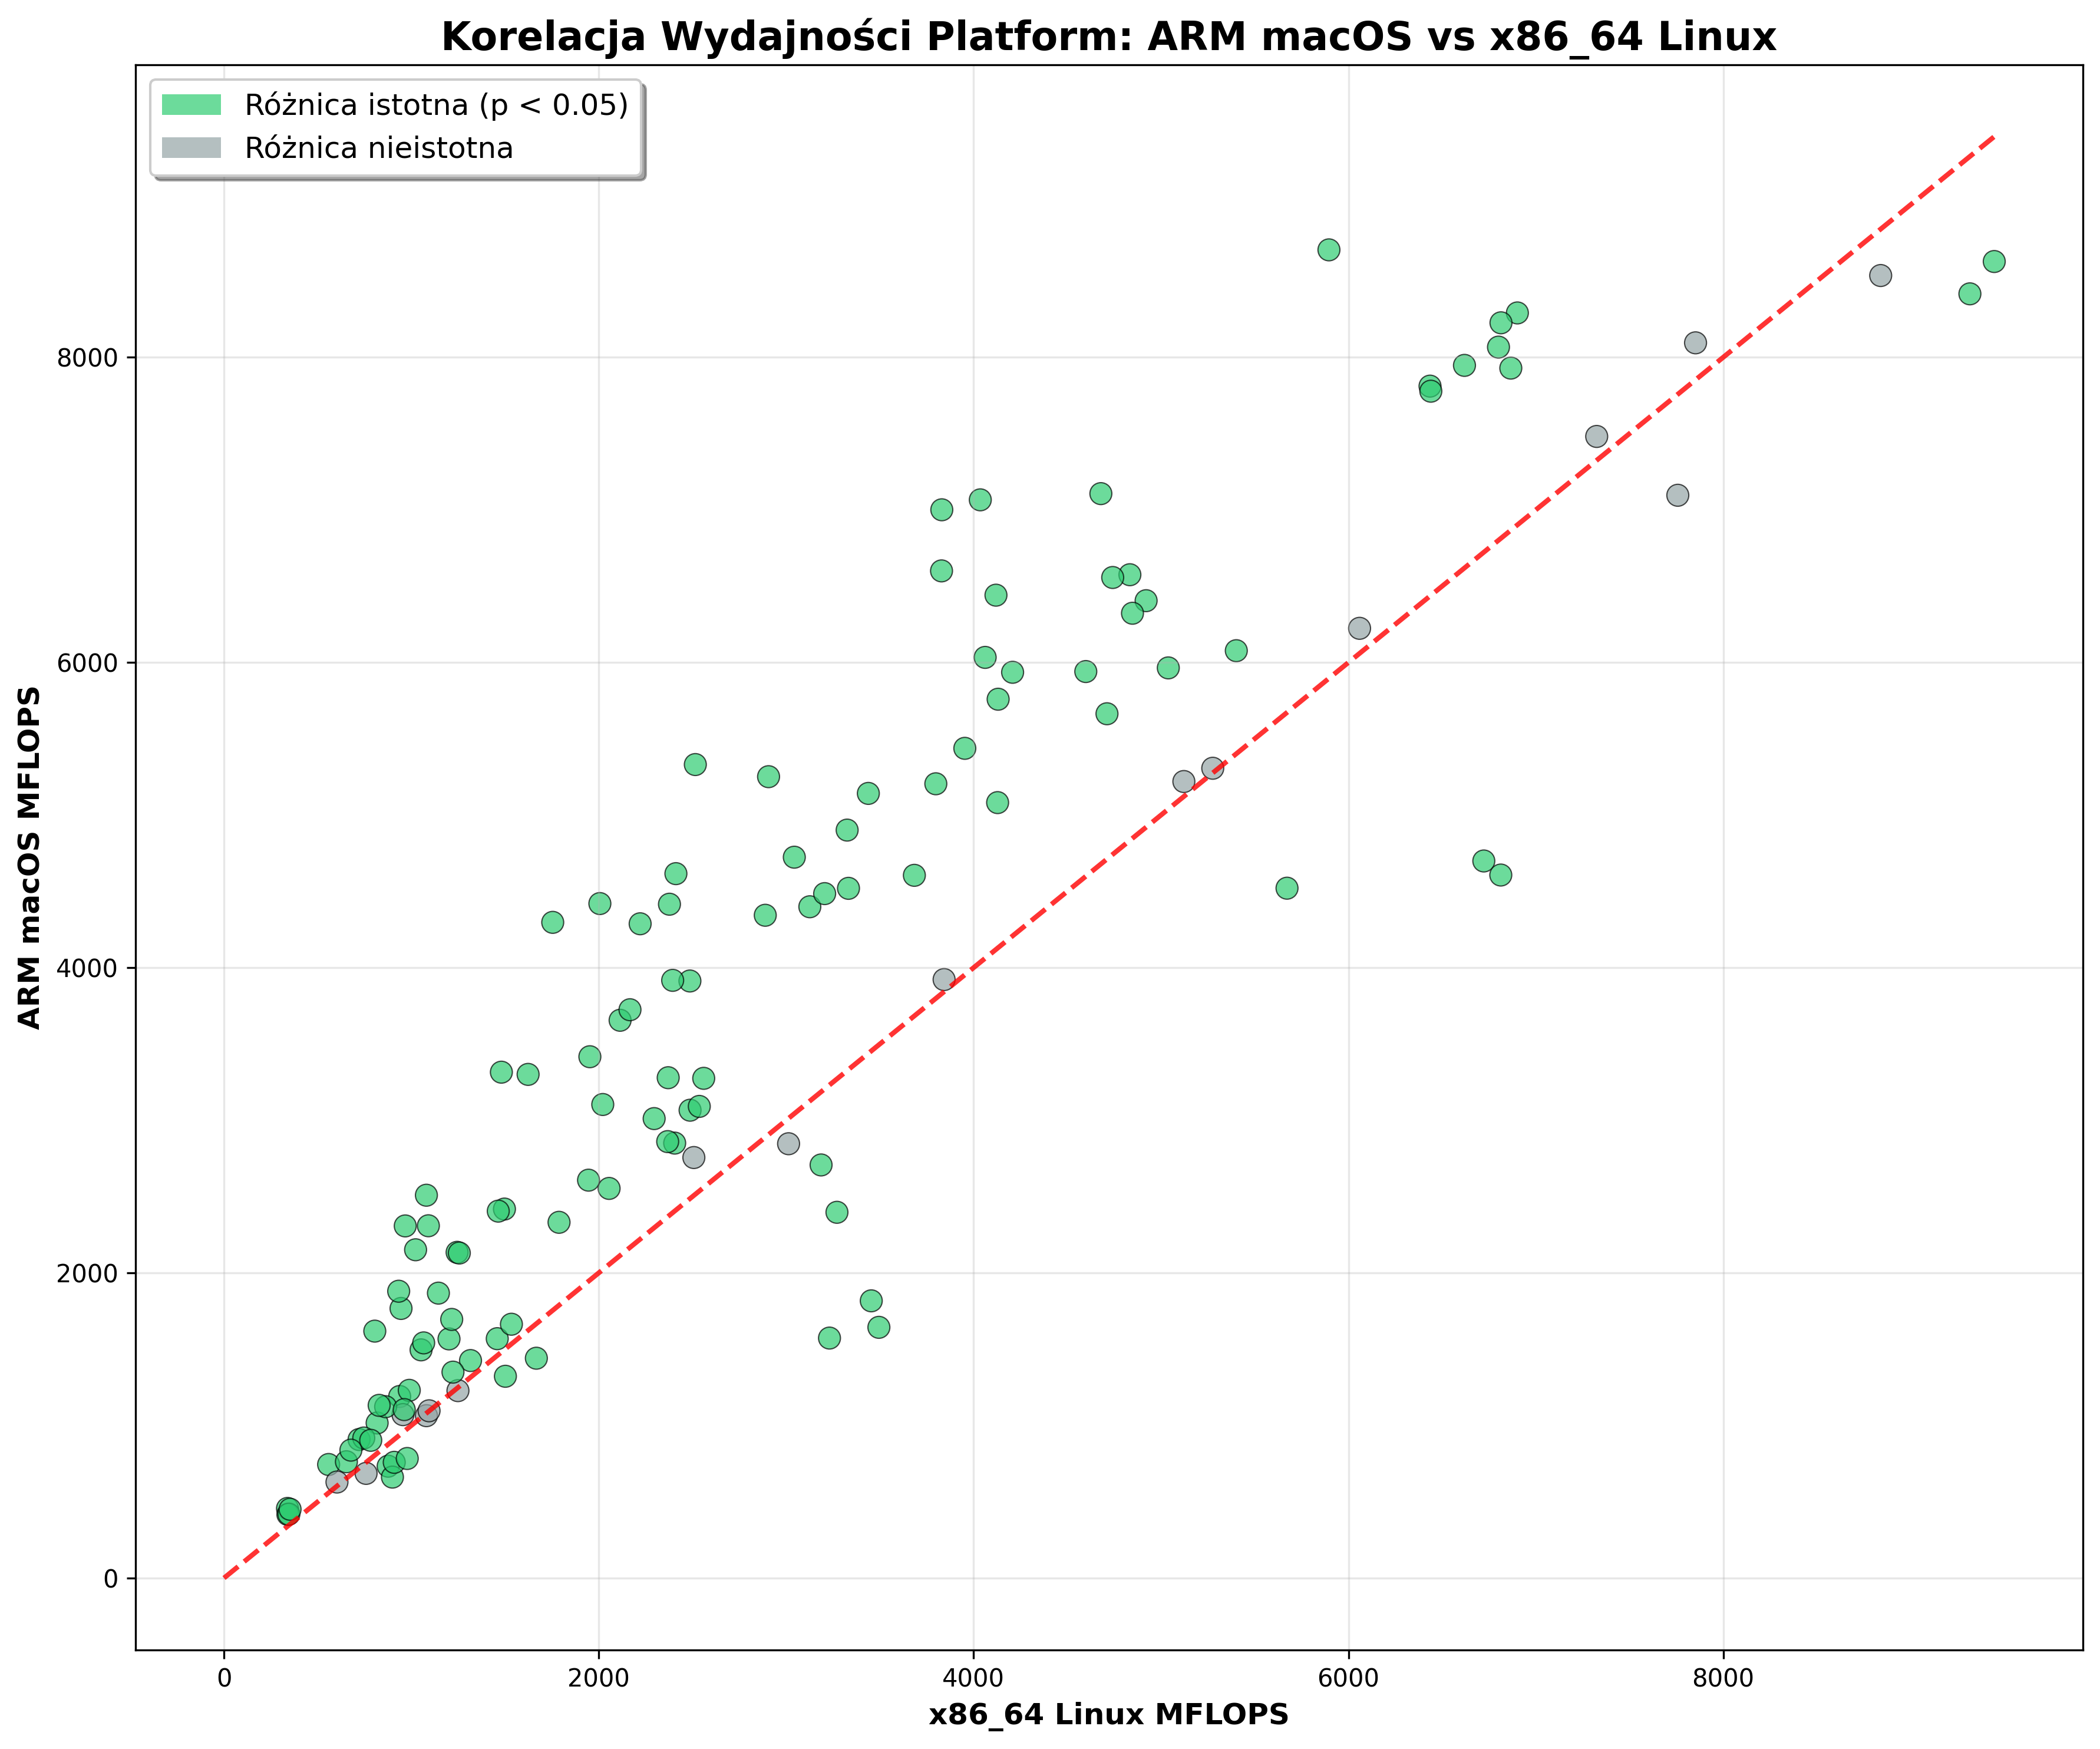
\includegraphics[width=\textwidth]{analiza/images/parallel/cg/compare/cg_analiza_istotnosci_statystycznej.png}
    \caption{Analiza istotności statystycznej benchmarku CG dla platform ARM64 i x86\_64}
    \label{cg_analiza_istotnosci_statystycznej}
\end{figure}
Na wykresie - rysunek \ref{cg_analiza_istotnosci_statystycznej} zaprezentowano korelację wydajności z uwzględnieniem istotności statystycznej (p < 0.05). Zdecydowana większość punktów (zielone oznaczenia) wskazuje na istotne różnice wydajności między platformami. Dla kilku przypadków (oznaczenia szare) różnica nie była statystycznie znacząca. Potwierdza to tezę, że platforma ARM macOS w większości przypadków przewyższa x86\_64 Linux, nie tylko nominalnie, ale również z punktu widzenia statystycznej wiarygodności wyników.